%==============================================================================
% Barrier Certificate Synthesis via Positivstellensatz:
% From Semantic Verification to Algebraic Proof Search
% in the Category of Polynomial Dynamical Systems
%==============================================================================

\documentclass[11pt,a4paper]{article}

\usepackage[utf8]{inputenc}
\usepackage[T1]{fontenc}
\usepackage{amsmath,amssymb,amsthm}
\usepackage{stmaryrd}
\usepackage{mathtools}
\usepackage{tikz}
\usepackage{tikz-cd}
\usetikzlibrary{positioning,arrows.meta,shapes.geometric,calc,decorations.pathmorphing}
\usepackage{hyperref}
\usepackage{cleveref}
\usepackage{booktabs}
\usepackage{enumitem}
\usepackage{geometry}
\usepackage{algorithm}
\usepackage{algpseudocode}
\usepackage{xcolor}
\usepackage{pgfplots}
\pgfplotsset{compat=1.18}

\geometry{margin=1in}

% Theorem environments
\theoremstyle{plain}
\newtheorem{theorem}{Theorem}[section]
\newtheorem{lemma}[theorem]{Lemma}
\newtheorem{proposition}[theorem]{Proposition}
\newtheorem{corollary}[theorem]{Corollary}

\theoremstyle{definition}
\newtheorem{definition}[theorem]{Definition}
\newtheorem{example}[theorem]{Example}
\newtheorem{construction}[theorem]{Construction}
\newtheorem{problem}[theorem]{Problem}

\theoremstyle{remark}
\newtheorem{remark}[theorem]{Remark}
\newtheorem{openproblem}[theorem]{Open Problem}

% Notation
\newcommand{\R}{\mathbb{R}}
\newcommand{\Z}{\mathbb{Z}}
\newcommand{\N}{\mathbb{N}}
\newcommand{\Q}{\mathbb{Q}}
\newcommand{\Sym}{\mathbb{S}}
\newcommand{\StateSpace}{\mathcal{S}}
\newcommand{\PolyRing}{\mathcal{R}}
\newcommand{\SOS}{\Sigma}
\newcommand{\PSD}{\mathcal{P}}
\newcommand{\Barrier}{\mathcal{B}}
\newcommand{\Reach}{\operatorname{Reach}}
\newcommand{\Safe}{\operatorname{Safe}}
\newcommand{\Unsafe}{\operatorname{Unsafe}}
\newcommand{\Init}{\operatorname{Init}}
\newcommand{\Trans}{\operatorname{Trans}}
\newcommand{\Target}{\operatorname{Target}}
\newcommand{\Inv}{\operatorname{Inv}}
\newcommand{\Cone}{\operatorname{Cone}}
\newcommand{\Ideal}{\operatorname{Ideal}}
\newcommand{\Preorder}{\operatorname{Preorder}}
\newcommand{\Sat}{\operatorname{Sat}}
\newcommand{\Pre}{\operatorname{Pre}}
\newcommand{\Post}{\operatorname{Post}}
\newcommand{\pre}{\mathrm{pre}}
\newcommand{\post}{\mathrm{post}}
\newcommand{\WP}{\operatorname{WP}}
\newcommand{\SP}{\operatorname{SP}}
\newcommand{\sem}[1]{\llbracket #1 \rrbracket}
\newcommand{\degree}{\operatorname{deg}}
\newcommand{\tr}{\operatorname{tr}}
\newcommand{\interior}{\operatorname{int}}
\newcommand{\closure}{\operatorname{cl}}
\newcommand{\boundary}{\partial}
\DeclareMathOperator{\Hom}{Hom}
\DeclareMathOperator{\id}{id}
\DeclareMathOperator{\Spec}{Spec}
\DeclareMathOperator{\Mor}{Mor}
\DeclareMathOperator{\conv}{conv}
\DeclareMathOperator{\diag}{diag}
\DeclareMathOperator{\rank}{rank}
\DeclareMathOperator{\New}{New}

% Colored boxes for key insights (using simple fbox-based approach)
\newenvironment{keyinsight}{%
  \par\vspace{0.5em}\noindent\fbox{\parbox{\dimexpr\textwidth-2\fboxsep-2\fboxrule}{\textbf{Key Insight.} 
}{%
  }}\par\vspace{0.5em}%
}

\newenvironment{paradigmshift}{%
  \par\vspace{0.5em}\noindent\fbox{\parbox{\dimexpr\textwidth-2\fboxsep-2\fboxrule}{\textbf{Paradigm Shift.} 
}{%
  }}\par\vspace{0.5em}%
}

\title{%
    \textbf{Barrier Certificate Synthesis via Positivstellensatz} \\[0.3em]
    \Large From Semantic Verification to Algebraic Proof Search \\
    in the Category of Polynomial Dynamical Systems \\[0.5em]
    \large Lyapunov Functions $\cdot$ Sum-of-Squares Hierarchies $\cdot$ \\
    Certified Invariant Discovery
}

\author{QSAT Research Group}
\date{December 2025}

\begin{document}
\maketitle

\begin{abstract}
We develop a categorical framework for \emph{barrier certificate synthesis} as the 
central verification primitive for polynomial dynamical systems. Building on the 
semialgebraic semantics of program verification, we observe that the traditional 
approach---encoding program semantics and checking safety---underutilizes the 
power of real algebraic geometry. We propose inverting the problem: rather than 
\emph{verifying} that a known property holds, we \emph{synthesize} an algebraic 
witness (the barrier certificate) that \emph{proves} safety.

The key mathematical contributions are:
\begin{itemize}[nosep]
    \item A categorical characterization of barrier certificates as morphisms in a 
        category $\mathbf{PolySafe}$ whose objects are safety problems and whose 
        morphisms are separating polynomials.
    \item A constructive connection between the Positivstellensatz and barrier 
        existence, showing that barrier synthesis reduces to sum-of-squares (SOS) 
        programming over coefficient spaces.
    \item A degree stratification theory establishing when finite-degree barriers 
        suffice, with explicit bounds for polynomial transition systems.
    \item A completeness theorem for the SOS hierarchy: if a polynomial barrier 
        exists at degree $d$, SOS relaxation at degree $\lceil d/2 \rceil$ finds it.
\end{itemize}

The framework unifies loop invariant discovery, Lyapunov function synthesis, and 
reachability analysis under a single algebraic umbrella, yielding a principled 
approach to certified bug detection that transcends pattern matching.
\end{abstract}

\tableofcontents
\newpage

%==============================================================================
\part{Foundations: The Algebra of Safety}
%==============================================================================

%==============================================================================
\section{Introduction: The Synthesis Paradigm}
\label{sec:intro}
%==============================================================================

\subsection{From Verification to Synthesis}

Traditional program verification proceeds in three steps:
\begin{enumerate}
    \item \textbf{Model}: Extract a mathematical model from the program.
    \item \textbf{Specify}: Express the safety property as a logical formula.
    \item \textbf{Check}: Verify that the model satisfies the specification.
\end{enumerate}

This \emph{verification} paradigm has a fundamental limitation: step (3) requires 
either exhaustive exploration (infeasible for infinite state spaces) or 
human-provided invariants (limiting automation).

\begin{paradigmshift}
We propose replacing \textbf{Check} with \textbf{Synthesize}: automatically 
discover an algebraic object (the barrier certificate) that \emph{proves} safety 
by construction. The existence of this object is equivalent to safety, but the 
object itself is a witness that can be verified independently.
\end{paradigmshift}

\subsection{Why Barrier Certificates?}

Consider a simple loop:
\begin{verbatim}
    while x > 0:
        x = x - 1
\end{verbatim}

The property ``$x \geq 0$ is invariant'' can be verified by:
\begin{itemize}
    \item \textbf{Checking}: Unroll the loop or find a human-provided invariant.
    \item \textbf{Synthesizing}: Find $B(x) = x$ and verify that $B \geq 0$ is 
        preserved by the loop body.
\end{itemize}

The synthesized $B$ serves dual purposes: (1) it proves safety, and (2) it 
explains \emph{why} the program is safe (the value $x$ is a natural ``progress 
measure'').

\subsection{Contributions and Outline}

This paper develops the mathematical theory of barrier certificate synthesis:

\begin{enumerate}
    \item \textbf{Section~\ref{sec:polynomial-dynamics}}: We define polynomial 
        dynamical systems and the safety problem categorically.
    
    \item \textbf{Section~\ref{sec:barrier-theory}}: We introduce barrier 
        certificates and prove the fundamental separation theorem.
    
    \item \textbf{Section~\ref{sec:sos}}: We connect barrier existence to the 
        Positivstellensatz and develop SOS synthesis.
    
    \item \textbf{Section~\ref{sec:degree-bounds}}: We establish degree bounds 
        and completeness results.
    
    \item \textbf{Section~\ref{sec:categorical}}: We construct the category 
        $\mathbf{PolySafe}$ and characterize barrier morphisms.
    
    \item \textbf{Section~\ref{sec:hierarchy}}: We develop the SOS hierarchy 
        and refinement procedures.
    
    \item \textbf{Section~\ref{sec:applications}}: We instantiate the framework 
        for specific bug types.
\end{enumerate}

%==============================================================================
\section{Polynomial Dynamical Systems}
\label{sec:polynomial-dynamics}
%==============================================================================

\subsection{State Spaces and Transitions}

\begin{definition}[Polynomial State Space]
\label{def:poly-state-space}
A \emph{polynomial state space} is a pair $(\StateSpace, \PolyRing)$ where:
\begin{itemize}
    \item $\StateSpace \subseteq \R^n$ is a basic semialgebraic set, i.e., 
        $\StateSpace = \{x \in \R^n : g_1(x) \geq 0, \ldots, g_m(x) \geq 0\}$ 
        for polynomials $g_i \in \R[x_1, \ldots, x_n]$.
    \item $\PolyRing = \R[x_1, \ldots, x_n]$ is the polynomial ring of 
        \emph{observables} on $\StateSpace$.
\end{itemize}
\end{definition}

\begin{definition}[Polynomial Transition System]
\label{def:pts}
A \emph{polynomial transition system} (PTS) is a tuple 
$\mathcal{P} = (\StateSpace, \Init, \Trans, \Unsafe)$ where:
\begin{itemize}
    \item $\StateSpace \subseteq \R^n$ is a polynomial state space.
    \item $\Init \subseteq \StateSpace$ is a semialgebraic set of initial states.
    \item $\Trans \subseteq \StateSpace \times \StateSpace$ is a semialgebraic 
        transition relation.
    \item $\Unsafe \subseteq \StateSpace$ is a semialgebraic set of unsafe states.
\end{itemize}
\end{definition}

\begin{remark}[Semialgebraic Encoding]
Each component admits a polynomial encoding:
\begin{align}
    \Init &= \{x : p_{\Init}(x) \geq 0\} \\
    \Trans &= \{(x, x') : p_{\Trans}(x, x') \geq 0\} \\
    \Unsafe &= \{x : p_{\Unsafe}(x) \geq 0\}
\end{align}
where the $p_\bullet$ are vectors of polynomials defining the sets via 
conjunctions/disjunctions of polynomial inequalities.
\end{remark}

\subsection{Reachability and Safety}

\begin{definition}[Reachable States]
\label{def:reach}
For a PTS $\mathcal{P}$, define the reachable set inductively:
\begin{align}
    \Reach^0(\mathcal{P}) &= \Init \\
    \Reach^{k+1}(\mathcal{P}) &= \Reach^k(\mathcal{P}) \cup 
        \{x' : \exists x \in \Reach^k(\mathcal{P}), (x, x') \in \Trans\} \\
    \Reach(\mathcal{P}) &= \bigcup_{k \geq 0} \Reach^k(\mathcal{P})
\end{align}
\end{definition}

\begin{definition}[Safety Problem]
\label{def:safety}
A PTS $\mathcal{P}$ is \emph{safe} if $\Reach(\mathcal{P}) \cap \Unsafe = \emptyset$.
The \emph{safety problem} is to determine whether $\mathcal{P}$ is safe.
\end{definition}

\begin{theorem}[Undecidability of General Safety]
\label{thm:undecidable}
The safety problem for polynomial transition systems with polynomial 
degree $\geq 2$ is undecidable.
\end{theorem}

\begin{proof}[Proof sketch]
Reduction from the halting problem for two-counter machines, which can be 
encoded as quadratic polynomial updates on $\R^2$.
\end{proof}

\begin{remark}
Despite undecidability of the general problem, \emph{barrier certificates} 
provide a sound (but incomplete) decision procedure: if a barrier exists, we 
can find it; if we find one, safety is guaranteed.
\end{remark}

%==============================================================================
\section{Rust-Specific Polynomial Encodings: Type System and Memory Model}
\label{sec:rust-polynomial-encoding}
%==============================================================================

\subsection{Motivation: Rust's Algebraic Safety Guarantees}

Rust's type system enforces memory safety through a combination of affine types 
(ownership), region-based lifetimes, and borrow checking. These mechanisms can be 
precisely encoded as polynomial constraints in our framework, enabling automated 
verification without relying on pattern matching or heuristics.

\begin{keyinsight}
Rust's ownership system corresponds to a \emph{polynomial flow network} where 
variables represent resource ownership states, and transitions encode moves, 
borrows, and drops. Barrier certificates in this encoding detect use-after-free, 
double-free, and aliasing violations by proving polynomial inequalities that 
contradict Rust's safety invariants.
\end{keyinsight}

\subsection{Ownership as Polynomial State Variables}

\begin{definition}[Ownership State Encoding]
\label{def:ownership-encoding}
For a Rust variable $v$ of type $T$, we introduce polynomial state variables:
\begin{align}
    \omega_v &\in \{0, 1\} \quad \text{(ownership indicator: 1 = owned, 0 = moved)} \\
    \beta_v &\in \N \quad \text{(borrow count: number of active borrows)} \\
    \mu_v &\in \{0, 1\} \quad \text{(mutability: 1 = mutable borrow active, 0 = none)} \\
    \lambda_v &\in \R_{\geq 0} \quad \text{(lifetime bound: remaining scope duration)}
\end{align}

The \emph{ownership polynomial} for $v$ is:
\begin{equation}
    \Omega_v(x) = \omega_v \cdot (1 - \mu_v \cdot \beta_v) \cdot \lambda_v
\end{equation}

Valid states satisfy $\Omega_v(x) \in \{0\} \cup [\epsilon, \infty)$ for small $\epsilon > 0$.
\end{definition}

\begin{proposition}[Ownership Preservation]
\label{prop:ownership-preservation}
Let $\Trans_{\text{move}}(v \to w)$ denote the transition polynomial for moving 
$v$ to $w$. Then:
\begin{equation}
    \Trans_{\text{move}}(x, x') = \begin{cases}
        (\omega_v = 1) \wedge (\omega'_w = 1) \wedge (\omega'_v = 0) & \text{if legal} \\
        \text{undefined (barrier violated)} & \text{if } \omega_v = 0
    \end{cases}
\end{equation}

The barrier certificate $B_{\text{ownership}}(x) = \sum_v \omega_v$ is non-increasing 
under legal moves and violates $B \geq 0$ under use-after-move.
\end{proposition}

\begin{proof}
A move transition decreases $\omega_v$ from 1 to 0 and increases $\omega_w$ from 0 to 1, 
preserving the sum. Attempting to use $v$ after move (when $\omega_v = 0$) requires 
accessing a state where $\omega_v \cdot \text{(operation)} < 0$, violating the barrier.
\end{proof}

\subsection{Borrow Checking as Semialgebraic Constraints}

\begin{definition}[Borrow Transition Polynomials]
\label{def:borrow-trans}
For an immutable borrow $\&v$, the transition is:
\begin{align}
    \Trans_{\text{borrow-imm}}(x, x') &= (\omega_v = 1) \wedge (\mu_v = 0) \wedge (\beta'_v = \beta_v + 1) \\
    \intertext{For a mutable borrow $\&\text{mut } v$:}
    \Trans_{\text{borrow-mut}}(x, x') &= (\omega_v = 1) \wedge (\beta_v = 0) \wedge (\mu'_v = 1) \wedge (\beta'_v = 1)
\end{align}

The \emph{borrow invariant polynomial} is:
\begin{equation}
    I_{\text{borrow}}(x) = \prod_v \left[ (1 - \mu_v)(1 + \beta_v) + \mu_v \cdot \mathbb{1}_{\{\beta_v = 1\}} \right]
\end{equation}
where $\mathbb{1}_{\{\beta_v = 1\}} = 1 - (\beta_v - 1)^2$ is the indicator polynomial.
\end{definition}

\begin{theorem}[Aliasing Detection via Barrier Certificates]
\label{thm:aliasing-barrier}
Let $\mathcal{P}$ be the PTS encoding a Rust program with variables $V$. Define:
\begin{equation}
    B_{\text{alias}}(x) = \sum_{v \in V} \left[ \mu_v \cdot \beta_v + \frac{1}{2}\mu_v^2 - \frac{3}{2}\mu_v \right]
\end{equation}

Then $B_{\text{alias}}(x) < 0$ if and only if there exists $v$ with $\mu_v = 1$ and $\beta_v > 1$, 
corresponding to a mutable borrow with additional active borrows (aliasing violation).

Furthermore, $B_{\text{alias}}$ is a barrier certificate: along any valid Rust execution trace,
$B_{\text{alias}}(x(t)) \geq 0$ for all $t$, and violation points are exactly the unsafe states.
\end{theorem}

\begin{proof}
For $\mu_v = 1$ (mutable borrow active), Rust's rules require $\beta_v = 1$ exactly. 
Substituting into $B_{\text{alias}}$:
\begin{align}
    B_{\text{alias}} &= \mu_v \cdot \beta_v + \frac{1}{2}\mu_v^2 - \frac{3}{2}\mu_v \\
    &= 1 \cdot \beta_v + \frac{1}{2} - \frac{3}{2} \\
    &= \beta_v - 1
\end{align}

For $\beta_v = 1$: $B_{\text{alias}} = 0$ (boundary of safe region). \\
For $\beta_v > 1$: $B_{\text{alias}} > 0$ (safe). \\
For $\beta_v < 1$: $B_{\text{alias}} < 0$ (impossible since $\beta_v \in \N$). \\
For $\beta_v = 0$: $\mu_v$ must be 0, so $B_{\text{alias}} = 0$ (safe).

The violation $\beta_v > 1 \wedge \mu_v = 1$ makes $B_{\text{alias}} > 0$ grow, but this 
configuration is unreachable from valid initial states under $\Trans_{\text{borrow}}$. 
Reaching it requires a buggy transition, which the barrier detects.
\end{proof}

\subsection{Lifetime Analysis via Temporal Polynomial Dynamics}

\begin{definition}[Lifetime Polynomial System]
\label{def:lifetime-poly}
For each Rust lifetime parameter $'a$, introduce a continuous-time variable 
$\tau_a \in \R_{\geq 0}$ representing the remaining scope duration. The dynamics are:
\begin{equation}
    \frac{d\tau_a}{dt} = -1, \quad \tau_a(0) = \text{static-scope-bound}
\end{equation}

For a borrow $r: \&'a T$, the \emph{lifetime constraint polynomial} is:
\begin{equation}
    L_r(x, t) = \tau_a(t) - \epsilon_{\text{margin}}
\end{equation}

A use-after-free occurs when code accesses $r$ at time $t$ where $L_r(x, t) < 0$.
\end{definition}

\begin{theorem}[Lifetime Barrier for Use-After-Free]
\label{thm:lifetime-barrier}
Define the global lifetime barrier:
\begin{equation}
    B_{\text{life}}(x, t) = \min_{r \in \text{Refs}} \left[ \omega_r \cdot L_r(x, t) + (1 - \omega_r) \cdot M \right]
\end{equation}
where $M$ is a large constant and $\omega_r$ indicates whether reference $r$ is active.

Then $B_{\text{life}} < 0$ detects use-after-free: accessing $r$ when $\tau_a \leq 0$.

Moreover, $B_{\text{life}}$ satisfies the barrier certificate condition:
\begin{equation}
    \frac{dB_{\text{life}}}{dt} = -\sum_{r \text{ active}} \omega_r \leq 0
\end{equation}
making it a valid Lyapunov-like certificate for temporal safety.
\end{theorem}

\subsection{Integer Overflow in Rust's Type System}

\begin{definition}[Bounded Integer Polynomial Encoding]
\label{def:int-overflow-poly}
For Rust type \texttt{u32}, represent values as $n \in [0, 2^{32} - 1]$. Operations 
encode as polynomials with overflow detection:
\begin{align}
    \text{checked\_add}(n, m) &\to n' = n + m, \quad \text{with barrier } B_+ = (2^{32} - 1) - n' \\
    \text{checked\_mul}(n, m) &\to n' = n \cdot m, \quad \text{with barrier } B_\times = (2^{32} - 1) - n'
\end{align}

Overflow occurs when $B_+ < 0$ or $B_\times < 0$, i.e., when the result exceeds $2^{32} - 1$.
\end{definition}

\begin{proposition}[Polynomial Overflow Barrier]
\label{prop:overflow-barrier}
For Rust arithmetic operation $n \oplus m$ where $\oplus \in \{+, \times\}$, define:
\begin{equation}
    B_{\oplus}(n, m) = (2^{32} - 1 - n) \cdot (2^{32} - 1 - m) - \epsilon \cdot n \cdot m
\end{equation}

For $\epsilon = 2^{-32}$, this polynomial is positive in the safe region 
$[0, 2^{32} - 1]^2$ and becomes negative precisely when $n \oplus m > 2^{32} - 1$.

The barrier certificate synthesis problem reduces to finding $\epsilon$ such that:
\begin{equation}
    B_{\oplus}(n, m) \in \SOS + \Ideal(n \cdot m - 2^{32})
\end{equation}
\end{proposition}

\subsection{Pattern Matching Exhaustiveness via Polynomial Covers}

\begin{definition}[Match Arm Coverage Polynomial]
\label{def:match-coverage}
For a Rust \texttt{match} expression on value $v: T$ with arms $\{A_1, \ldots, A_k\}$, 
encode each arm's pattern as a semialgebraic set:
\begin{equation}
    A_i = \{v : p_i(v) \geq 0\}
\end{equation}

The \emph{coverage polynomial} is:
\begin{equation}
    C_{\text{match}}(v) = \sum_{i=1}^k \mathbb{1}_{A_i}(v) \cdot w_i
\end{equation}
where $\mathbb{1}_{A_i}$ is the indicator polynomial and $w_i > 0$ are weights.

Exhaustiveness requires $C_{\text{match}}(v) > 0$ for all $v \in T$.
\end{definition}

\begin{theorem}[Exhaustiveness as Positivstellensatz Certificate]
\label{thm:match-exhaustive}
A match expression is exhaustive if and only if:
\begin{equation}
    1 \in \Ideal(p_1, \ldots, p_k) + \Preorder(g_1, \ldots, g_m)
\end{equation}
where $g_j$ define the type $T$ as a basic semialgebraic set.

This admits a sum-of-squares relaxation: find $\sigma_0, \ldots, \sigma_k \in \SOS$ such that:
\begin{equation}
    1 = \sigma_0 + \sum_{i=1}^k p_i \cdot \sigma_i + \sum_{j=1}^m g_j \cdot \tau_j
\end{equation}

The existence of such $\{\sigma_i\}$ certificates exhaustiveness computationally.
\end{theorem}

\subsection{Drop Checker and Destructor Safety}

\begin{definition}[Drop Flag Polynomial]
\label{def:drop-flag-poly}
For each Rust value $v$ with a custom \texttt{Drop} implementation, introduce:
\begin{align}
    \delta_v &\in \{0, 1\} \quad \text{(drop flag: 1 = needs drop, 0 = dropped)} \\
    \rho_v &\in \N \quad \text{(reference count from borrows)}
\end{align}

The \emph{drop safety polynomial} is:
\begin{equation}
    D_v(x) = \delta_v \cdot (1 - \rho_v)
\end{equation}

Drop safety requires: drop occurs only when $\delta_v = 1$ and $\rho_v = 0$.
\end{definition}

\begin{proposition}[Double-Drop Detection]
\label{prop:double-drop}
Define the barrier certificate:
\begin{equation}
    B_{\text{drop}}(x) = \sum_v \left[ \delta_v - \frac{1}{2}(\delta_v - 1)^2 \right]
\end{equation}

A double-drop (calling drop on $v$ when $\delta_v = 0$) violates $B_{\text{drop}} \geq 0$, 
as the term becomes negative. Along valid execution traces:
\begin{equation}
    \Delta B_{\text{drop}} = -\sum_{\text{drops}} 1 \leq 0
\end{equation}
making it a valid barrier certificate for drop safety.
\end{proposition}

\subsection{Panic Safety and Unwinding Barriers}

\begin{definition}[Panic State Polynomial]
\label{def:panic-poly}
Introduce a global panic indicator $\pi \in \{0, 1\}$ where $\pi = 1$ means 
the program is unwinding. For each function $f$, define its \emph{panic potential}:
\begin{equation}
    P_f(x) = \sum_{\text{panic points } p} \text{dist}(x, p)^{-2}
\end{equation}

A panic barrier certificate is:
\begin{equation}
    B_{\text{panic}}(x) = (1 - \pi) \cdot M - P_f(x)
\end{equation}

where $M$ is chosen such that $B_{\text{panic}} > 0$ in panic-free regions.
\end{definition}

\begin{theorem}[Invariant Preservation During Unwinding]
\label{thm:unwind-invariant}
Let $I(x)$ be an invariant polynomial. Define the \emph{unwind-safe barrier}:
\begin{equation}
    B_{\text{unwind}}(x) = (1 - \pi) \cdot I(x) + \pi \cdot W(x)
\end{equation}

where $W(x)$ is the \emph{unwinding invariant} (weaker than $I$). Then:
\begin{equation}
    B_{\text{unwind}}(x(t)) \geq 0 \quad \forall t \implies \text{panic-safe}
\end{equation}

Rust's unwinding guarantees that drop glue maintains $W(x) \geq 0$ along unwind paths.
\end{theorem}

\subsection{Trait Coherence and Method Resolution as Polynomial Constraints}

\begin{definition}[Trait Implementation Polynomial]
\label{def:trait-impl-poly}
For a trait \texttt{Trait} with method \texttt{fn method(self)} and implementations 
on types $T_1, \ldots, T_k$, represent the type space as $\R^n$ where each $T_i$ 
occupies a semialgebraic region $\mathcal{T}_i \subseteq \R^n$.

The \emph{trait coherence polynomial} is:
\begin{equation}
    \Theta_{\text{Trait}}(x) = \sum_{i=1}^k \mathbb{1}_{\mathcal{T}_i}(x) \cdot \sigma_i(x)
\end{equation}

where $\sigma_i \in \SOS$ are sum-of-squares polynomials ensuring uniqueness:
\begin{equation}
    \mathbb{1}_{\mathcal{T}_i}(x) \cdot \mathbb{1}_{\mathcal{T}_j}(x) = 0 \quad \forall i \neq j
\end{equation}
\end{definition}

\begin{proposition}[Orphan Rule as Semialgebraic Separation]
\label{prop:orphan-rule}
Rust's orphan rule (preventing overlapping trait implementations) translates to:
\begin{equation}
    \Cone(\mathcal{T}_i \cap \mathcal{T}_j) = \{0\} \quad \forall i \neq j
\end{equation}

This is a polynomial separation condition solvable via barrier synthesis: find 
$B_{ij}(x)$ such that:
\begin{equation}
    B_{ij}(x) > 0 \text{ on } \mathcal{T}_i, \quad B_{ij}(x) < 0 \text{ on } \mathcal{T}_j
\end{equation}

The existence of $B_{ij}$ for all pairs proves coherence.
\end{proposition}

\subsection{Generic Type Parameters and Monomorphization}

\begin{definition}[Parametric Polynomial Family]
\label{def:generic-poly-family}
For a generic Rust function \texttt{fn foo<T>(x: T) -> U}, the polynomial encoding 
is a \emph{family} indexed by type parameters:
\begin{equation}
    \mathcal{F}_{\text{foo}} = \{f_T : \R^{n_T} \to \R^{m_U}\}_{T \in \text{Types}}
\end{equation}

A trait bound \texttt{T: Trait} restricts $T$ to the semialgebraic subset:
\begin{equation}
    \mathcal{T}_{\text{Trait}} = \{T : \Theta_{\text{Trait}}(T) \geq 0\}
\end{equation}
\end{definition}

\begin{theorem}[Parametric Barrier Certificates]
\label{thm:parametric-barrier}
Let $B_T(x)$ be a barrier certificate for monomorphization $\text{foo}::<T>$. Then:
\begin{equation}
    B_{\text{generic}}(x, T) = \inf_{T \in \mathcal{T}_{\text{Trait}}} B_T(x)
\end{equation}

is a parametric barrier certificate valid for all valid instantiations. Computing 
this reduces to \emph{parametric polynomial optimization}:
\begin{equation}
    \min_{T, x} B_T(x) \quad \text{s.t.} \quad \Theta_{\text{Trait}}(T) \geq 0
\end{equation}

When $B_{\text{generic}} \geq 0$, the generic function is safe for all instantiations.
\end{theorem}

\subsection{Unsafe Blocks and Invariant Preservation}

\begin{definition}[Unsafe Context Polynomial]
\label{def:unsafe-context-poly}
An \texttt{unsafe} block suspends Rust's automatic checks, modeled by relaxing constraints. 
Introduce an unsafe flag $u \in \{0, 1\}$:
\begin{align}
    I_{\text{safe}}(x) &= \text{standard Rust invariants} \\
    I_{\text{unsafe}}(x) &= \text{weakened invariants (manual responsibility)}
\end{align}

The \emph{context-dependent invariant} is:
\begin{equation}
    I_{\text{total}}(x, u) = (1 - u) \cdot I_{\text{safe}}(x) + u \cdot I_{\text{unsafe}}(x)
\end{equation}
\end{definition}

\begin{theorem}[Unsafe Block Safety via Barrier Certificates]
\label{thm:unsafe-barrier}
For an unsafe block with pre-condition $P(x)$ and post-condition $Q(x)$, safety 
requires a barrier $B_{\text{unsafe}}(x)$ satisfying:
\begin{align}
    P(x) &\implies B_{\text{unsafe}}(x) \geq 0 \\
    B_{\text{unsafe}}(x') &\geq B_{\text{unsafe}}(x) - \epsilon \cdot \|x' - x\| \\
    B_{\text{unsafe}}(x) &\geq 0 \implies Q(x)
\end{align}

The second condition ensures the barrier doesn't decrease too quickly during the 
unsafe operations, maintaining safety margin. Finding such $B_{\text{unsafe}}$ via 
SOS synthesis certifies the unsafe block's correctness.
\end{theorem}

\subsection{Send and Sync Traits as Polynomial Thread-Safety Certificates}

\begin{definition}[Thread-Safety Polynomial]
\label{def:send-sync-poly}
For a type $T$, introduce concurrency state variables:
\begin{align}
    \theta_T &\in \N \quad \text{(thread count: number of threads with access)} \\
    \xi_T &\in \{0, 1\} \quad \text{(exclusive flag: 1 if mutation possible)}
\end{align}

The \texttt{Send} trait corresponds to:
\begin{equation}
    \Psi_{\text{Send}}(T) = 1 - \xi_T \cdot (\theta_T - 1) \geq 0
\end{equation}

The \texttt{Sync} trait corresponds to:
\begin{equation}
    \Psi_{\text{Sync}}(T) = (1 - \xi_T) \cdot \theta_T \geq 0
\end{equation}
\end{definition}

\begin{proposition}[Data Race Freedom via Barrier]
\label{prop:race-free-barrier}
Define the \emph{race-freedom barrier}:
\begin{equation}
    B_{\text{race}}(x) = \sum_{T} \left[ \xi_T \cdot \max(1 - \theta_T, 0) + (1 - \xi_T) \right]
\end{equation}

A data race (multiple threads with at least one writer) occurs when $\xi_T = 1$ and 
$\theta_T > 1$, which makes $B_{\text{race}} < 0$. For safe programs:
\begin{equation}
    B_{\text{race}}(x(t)) \geq 0 \quad \forall t
\end{equation}

The barrier synthesis problem: find $B_{\text{race}}$ in SOS form satisfying transition constraints.
\end{proposition}

\subsection{Pin and Unpin: Self-Referential Struct Safety}

\begin{definition}[Pin Safety Polynomial]
\label{def:pin-poly}
For a pinned value $v: Pin<P>$, introduce:
\begin{align}
    \phi_v &\in \{0, 1\} \quad \text{(pin status: 1 = pinned, 0 = unpinned)} \\
    \alpha_v &\in \R^n \quad \text{(memory address)} \\
    \kappa_v &\in \R_{\geq 0} \quad \text{(self-reference count)}
\end{align}

The \emph{pin invariant polynomial}:
\begin{equation}
    \Pi_v(x) = \phi_v \cdot \left( \|\alpha_v - \alpha_v^{\text{init}}\|^2 \cdot \kappa_v + (1 - \kappa_v) \right)
\end{equation}

Violation occurs when $\phi_v = 1$ (pinned), $\kappa_v > 0$ (self-referential), and 
$\alpha_v \neq \alpha_v^{\text{init}}$ (moved), making $\Pi_v > 0$ signal unsafety.
\end{definition}

\begin{theorem}[Pin Safety as Barrier Certificate]
\label{thm:pin-barrier}
The global pin safety barrier is:
\begin{equation}
    B_{\text{pin}}(x) = -\sum_v \Pi_v(x) + M \cdot \sum_v (1 - \phi_v)
\end{equation}

where $M$ is a large constant. Then $B_{\text{pin}} < 0$ precisely when a pinned 
self-referential value has been moved, violating safety.

For futures and async contexts, this extends to \emph{temporal pin barriers}:
\begin{equation}
    B_{\text{async}}(x, t) = B_{\text{pin}}(x) \cdot \prod_{\text{poll points}} (1 - \mathbb{1}_{\text{poll}}(t))
\end{equation}

ensuring pin safety persists across await points.
\end{theorem}

\subsection{Variance and Subtyping via Polynomial Functors}

\begin{definition}[Variance Polynomial]
\label{def:variance-poly}
For a generic type $F<T>$ with lifetime parameter $T = 'a$, encode variance as a 
polynomial functional:
\begin{align}
    \text{Covariant:} \quad &\mathcal{V}_F(\tau_a) = \tau_a \\
    \text{Contravariant:} \quad &\mathcal{V}_F(\tau_a) = -\tau_a \\
    \text{Invariant:} \quad &\mathcal{V}_F(\tau_a) = 0
\end{align}

Subtyping $'a \preceq 'b$ (lifetime $'a$ outlives $'b$) corresponds to:
\begin{equation}
    \tau_a - \tau_b \geq 0
\end{equation}
\end{definition}

\begin{proposition}[Variance Safety Barrier]
\label{prop:variance-barrier}
For a covariant type $F<'a>$, the variance barrier is:
\begin{equation}
    B_{\text{var}}(F, 'a, 'b) = (\tau_a - \tau_b) \cdot \mathcal{V}_F(\tau_a)
\end{equation}

Assigning $F<'a>$ to $F<'b>$ is safe iff $B_{\text{var}} \geq 0$. Contravariant and 
invariant cases adjust the polynomial accordingly. Synthesizing $B_{\text{var}}$ in 
SOS form certifies subtyping relations.
\end{proposition}

\subsection{Interior Mutability and Cell Types}

\begin{definition}[Interior Mutability Polynomial]
\label{def:cell-poly}
For \texttt{Cell<T>} and \texttt{RefCell<T>}, introduce:
\begin{align}
    \iota_v &\in \{0, 1\} \quad \text{(interior mutability flag)} \\
    \gamma_v &\in \N \quad \text{(borrow state: 0 = free, 1 = borrowed, 2 = mut borrowed)}
\end{align}

The \emph{cell safety polynomial}:
\begin{equation}
    C_v(x) = \iota_v \cdot \left[ 1 - \frac{(\gamma_v - 1)(\gamma_v - 2)}{2} \right]
\end{equation}

Valid states have $\gamma_v \in \{0, 1\}$ for \texttt{Cell} or $\gamma_v \in \{0, 1, 2\}$ 
for \texttt{RefCell} with dynamic checks ensuring single mutable borrow.
\end{definition}

\begin{proposition}[RefCell Panic Detection]
\label{prop:refcell-panic}
A \texttt{RefCell::borrow\_mut()} call when $\gamma_v > 0$ triggers panic. The barrier:
\begin{equation}
    B_{\text{refcell}}(x) = -\gamma_v \cdot (\gamma_v - 1)
\end{equation}

Attempting to acquire mutable borrow when $\gamma_v \geq 1$ makes $B_{\text{refcell}} < 0$, 
signaling a runtime panic. Static analysis via barrier synthesis detects potential 
panics by finding reachable states where $B_{\text{refcell}} < 0$.
\end{proposition}

\subsection{Const Generics and Compile-Time Polynomial Evaluation}

\begin{definition}[Const Generic Polynomial]
\label{def:const-generic-poly}
For \texttt{fn foo<const N: usize>()}, the polynomial family is indexed by integer parameters:
\begin{equation}
    \mathcal{F}_{\text{foo}} = \{f_N : \R^n \to \R^m\}_{N \in \N}
\end{equation}

Array bounds checking becomes polynomial constraint:
\begin{equation}
    \text{index } i < N \iff N - i - 1 \geq 0
\end{equation}
\end{definition}

\begin{theorem}[Const Generic Barrier Synthesis]
\label{thm:const-generic-barrier}
For a const generic function accessing array $A: [T; N]$ at index $i$, the barrier:
\begin{equation}
    B_N(i) = (N - 1 - i) \cdot i
\end{equation}

This is positive for $i \in [0, N-1]$ and negative outside. Parametric in $N$:
\begin{equation}
    \forall N \in \N, \quad B_N(i) \geq 0 \iff i \in [0, N-1]
\end{equation}

Synthesizing $B_N$ as a polynomial in both $i$ and $N$ certifies bounds safety across 
all instantiations.
\end{theorem}

\subsection{Macro Hygiene and Expansion Safety}

\begin{definition}[Macro Expansion Polynomial]
\label{def:macro-poly}
A Rust macro \texttt{macro\_rules! m} with expansion $E(x_1, \ldots, x_k)$ encodes as:
\begin{equation}
    M_{\text{expand}}(x, y) = E_{\text{poly}}(x) - y
\end{equation}

where $x$ are macro inputs and $y$ is the expansion result. Hygiene violations occur 
when free variables in $x$ collide with bindings in the expansion context.
\end{definition}

\begin{proposition}[Hygiene Barrier]
\label{prop:hygiene-barrier}
Define the \emph{name-collision polynomial}:
\begin{equation}
    H_{\text{macro}}(x, \text{ctx}) = \sum_{\text{vars } v} \mathbb{1}_{v \in x}(v) \cdot \mathbb{1}_{v \in \text{ctx}}(v)
\end{equation}

Hygiene requires $H_{\text{macro}} = 0$. Non-zero values indicate collision. Barrier 
synthesis finds separating polynomials proving $H_{\text{macro}} = 0$ under Rust's 
hygiene rules.
\end{proposition}

\subsection{Async/Await State Machines as Polynomial Automata}

\begin{definition}[Future State Polynomial]
\label{def:future-poly}
An \texttt{async fn} desugars to a state machine with states $\{S_0, S_1, \ldots, S_k\}$ 
corresponding to await points. Encode states as polynomial indicators:
\begin{align}
    \sigma &\in \{0, 1, \ldots, k\} \quad \text{(current state index)} \\
    \psi_i &= \prod_{j \neq i} \frac{\sigma - j}{i - j} \quad \text{(Lagrange basis for state } S_i\text{)}
\end{align}

The \emph{future transition polynomial}:
\begin{equation}
    F_{\text{trans}}(\sigma, \sigma', x, x') = \sum_{i=0}^{k-1} \psi_i(\sigma) \cdot \psi_{i+1}(\sigma') \cdot T_i(x, x')
\end{equation}

where $T_i$ is the transition polynomial from state $S_i$ to $S_{i+1}$.
\end{definition}

\begin{theorem}[Async Safety via Barrier Certificates]
\label{thm:async-barrier}
For an async function with pinned futures, define the \emph{async-safe barrier}:
\begin{equation}
    B_{\text{async}}(\sigma, x) = \sum_{i=0}^k \psi_i(\sigma) \cdot B_i(x)
\end{equation}

where each $B_i$ is a state-specific barrier. Safety requires:
\begin{align}
    B_{\text{async}}(\sigma, x) &\geq 0 \quad \text{(always safe)} \\
    F_{\text{trans}}(\sigma, \sigma', x, x') &\implies B_{\text{async}}(\sigma', x') \geq B_{\text{async}}(\sigma, x) - \epsilon
\end{align}

The second condition ensures barrier monotonicity across await points, preventing 
state corruption during suspension/resumption. This is polynomial in both discrete 
state $\sigma$ and continuous state $x$.
\end{theorem}

\begin{proposition}[Waker Safety Polynomial]
\label{prop:waker-poly}
A waker wake-up when the future is already completed violates safety. Introduce:
\begin{align}
    \omega &\in \{0, 1\} \quad \text{(waker validity: 1 = valid, 0 = consumed)} \\
    \chi &\in \{0, 1\} \quad \text{(future completion: 1 = done, 0 = pending)}
\end{align}

The waker safety polynomial:
\begin{equation}
    W_{\text{wake}}(\omega, \chi) = \omega \cdot (1 - \chi)
\end{equation}

Calling \texttt{wake()} requires $\omega = 1$ (waker valid) and $\chi = 0$ (future pending). 
After completion ($\chi = 1$), $W_{\text{wake}} = 0$, and further wakes violate the barrier.
\end{proposition}

\subsection{Closure Capture and Environment Polynomials}

\begin{definition}[Closure Environment Polynomial]
\label{def:closure-env-poly}
For a closure \texttt{|x| body}, the captured environment variables form a vector 
$\mathbf{e} = (e_1, \ldots, e_m)$. Each closure invocation acts on state $(x, \mathbf{e})$.

The capture mode (move, borrow, mut borrow) determines the polynomial encoding:
\begin{align}
    \text{FnOnce (move):} \quad &\mathcal{C}_{\text{once}}(\mathbf{e}, \omega) = \omega \cdot \|\mathbf{e}\|^2 \\
    \text{FnMut (mut borrow):} \quad &\mathcal{C}_{\text{mut}}(\mathbf{e}, \mu) = \mu \cdot \|\mathbf{e}\|^2 \\
    \text{Fn (shared borrow):} \quad &\mathcal{C}_{\text{fn}}(\mathbf{e}, \beta) = \beta \cdot \|\mathbf{e}\|^2
\end{align}

where $\omega, \mu, \beta$ are ownership/borrow flags as defined earlier.
\end{definition}

\begin{theorem}[Closure Invocation Safety via Barrier]
\label{thm:closure-barrier}
For an \texttt{FnOnce} closure, the barrier:
\begin{equation}
    B_{\text{FnOnce}}(\mathbf{e}, \omega, n) = \omega - n
\end{equation}

where $n$ is the number of invocations. After first call, $\omega = 0$ (moved), so 
$B_{\text{FnOnce}} < 0$ for subsequent calls, detecting the violation.

For \texttt{FnMut}, the barrier ensures exclusive access:
\begin{equation}
    B_{\text{FnMut}}(\mu, \beta) = \mu \cdot (1 - \beta) + (1 - \mu)
\end{equation}

Active mutable borrow ($\mu = 1$) requires no other borrows ($\beta = 0$).
\end{theorem}

\begin{proposition}[Capture-By-Move Detection]
\label{prop:capture-move}
A variable $v$ captured by move in closure $c$ must not be used in outer scope. 
The polynomial encoding:
\begin{equation}
    M_{\text{capture}}(v, c) = \omega_v^{\text{outer}} \cdot \omega_v^{\text{inner}}
\end{equation}

After capture, $\omega_v^{\text{outer}} = 0$ (moved out). Using $v$ in outer scope 
requires $\omega_v^{\text{outer}} = 1$, contradiction detected by $M_{\text{capture}} = 0$.

Barrier synthesis: find $B$ such that $B \geq 0$ and $M_{\text{capture}} = 0$ under 
valid program traces.
\end{proposition}

\subsection{Trait Objects and Dynamic Dispatch Polynomials}

\begin{definition}[Vtable Polynomial]
\label{def:vtable-poly}
A trait object \texttt{dyn Trait} has a vtable pointer $v \in \mathcal{V}$ (set of 
valid vtables). Encode as:
\begin{align}
    v_{\text{ptr}} &\in \R^n \quad \text{(vtable address)} \\
    v_{\text{type}} &\in \mathbb{T} \quad \text{(concrete type index)}
\end{align}

The \emph{vtable validity polynomial}:
\begin{equation}
    V_{\text{valid}}(v_{\text{ptr}}, v_{\text{type}}) = \sum_{T \in \text{Impls}} \mathbb{1}_{v_{\text{ptr}} = v_T}(v_{\text{ptr}}) \cdot \mathbb{1}_{v_{\text{type}} = T}(v_{\text{type}})
\end{equation}

where $v_T$ is the vtable for type $T$'s implementation.
\end{definition}

\begin{proposition}[Vtable Pointer Safety]
\label{prop:vtable-safety}
Calling a method through invalid vtable pointer violates safety. The barrier:
\begin{equation}
    B_{\text{vtable}}(v) = V_{\text{valid}}(v_{\text{ptr}}, v_{\text{type}}) - \epsilon
\end{equation}

For small $\epsilon > 0$, $B_{\text{vtable}} < 0$ when $v_{\text{ptr}}$ doesn't correspond 
to $v_{\text{type}}$'s vtable, detecting type confusion bugs.

This extends to \emph{object safety}: trait methods must satisfy polynomial constraints 
ensuring vtable compatibility:
\begin{equation}
    \text{Object-safe} \iff \forall T, \quad \Theta_{\text{Trait}}^T \text{ has finite polynomial encoding}
\end{equation}
\end{proposition}

\subsection{Slice Bounds and Iterator Safety}

\begin{definition}[Slice Polynomial]
\label{def:slice-poly}
For a slice \texttt{\&[T]} with length $\ell$ and index $i$, the bounds polynomial:
\begin{equation}
    S_{\text{bounds}}(i, \ell) = i \cdot (\ell - 1 - i)
\end{equation}

This is positive for $i \in [0, \ell - 1]$ and non-positive outside bounds.
\end{definition}

\begin{proposition}[Iterator Range Safety]
\label{prop:iterator-range}
An iterator \texttt{iter} over slice $s$ maintains index $i \in [0, \ell)$. The barrier:
\begin{equation}
    B_{\text{iter}}(i, \ell) = \min(i, \ell - 1 - i)
\end{equation}

Each \texttt{next()} call increments $i$ with precondition $i < \ell$. When $i = \ell$, 
iterator returns \texttt{None}, maintaining $B_{\text{iter}} \geq 0$ throughout.

For \texttt{Iterator::skip(n)}, the transition:
\begin{equation}
    T_{\text{skip}}(i, i', n) : i' = i + n \wedge B_{\text{iter}}(i', \ell) \geq 0
\end{equation}

Violating this (skipping past end) is caught by barrier synthesis as unsound.
\end{proposition}

\subsection{Atomic Operations and Memory Ordering Polynomials}

\begin{definition}[Atomic State Polynomial]
\label{def:atomic-poly}
For \texttt{AtomicU32} with value $a$ and memory order $o \in \{\text{Relaxed, Acquire, Release, AcqRel, SeqCst}\}$:
\begin{align}
    a &\in [0, 2^{32} - 1] \quad \text{(atomic value)} \\
    o &\in \{0, 1, 2, 3, 4\} \quad \text{(memory order encoding)}
\end{align}

The \emph{happens-before polynomial} for operations $op_1, op_2$:
\begin{equation}
    H_{\text{before}}(op_1, op_2) = (o_1 \geq 2) \wedge (o_2 \geq 1) \implies \tau_1 < \tau_2
\end{equation}

where $\tau_i$ are timestamps. Violations (data races) occur when $H_{\text{before}} = 0$ 
for conflicting operations.
\end{definition}

\begin{theorem}[Atomic Safety via Temporal Barrier]
\label{thm:atomic-barrier}
For concurrent atomic operations $\{op_i\}_{i=1}^k$, define:
\begin{equation}
    B_{\text{atomic}}(\mathbf{o}, \boldsymbol{\tau}) = \sum_{i < j} H_{\text{before}}(op_i, op_j) \cdot \mathbb{1}_{\text{conflict}}(i, j)
\end{equation}

where $\mathbb{1}_{\text{conflict}}(i, j) = 1$ if $op_i, op_j$ access same location 
with at least one write. Then:
\begin{equation}
    B_{\text{atomic}} \geq 0 \iff \text{no data race}
\end{equation}

Memory order constraints ensure $B_{\text{atomic}}$ remains positive, certifying race freedom.
\end{theorem}

\subsection{Type-State Programming via Polynomial Mode Transitions}

\begin{definition}[Type-State Polynomial]
\label{def:typestate-poly}
For a file handle \texttt{File} with states \{\texttt{Closed}, \texttt{Open}, \texttt{Locked}\}, 
encode as polynomial:
\begin{align}
    s &\in \{0, 1, 2\} \quad \text{(state: 0=Closed, 1=Open, 2=Locked)} \\
    \phi_s &= \prod_{j \neq s} \frac{x - j}{s - j} \quad \text{(Lagrange basis for state } s\text{)}
\end{align}

Operations have state-dependent preconditions:
\begin{align}
    \text{read}(f) &\text{ requires } s \in \{1, 2\} \iff \phi_1(s) + \phi_2(s) > 0 \\
    \text{close}(f) &\text{ requires } s = 1 \iff \phi_1(s) = 1
\end{align}
\end{definition}

\begin{theorem}[Type-State Barrier Synthesis]
\label{thm:typestate-barrier}
For type-state protocol $P$ with states $S$ and transitions $T$, the barrier:
\begin{equation}
    B_P(s, op) = \sum_{(s, op, s') \in T} \phi_s(s) \cdot \phi_{s'}(s')
\end{equation}

Protocol violations (invalid transitions) make $B_P = 0$. Valid traces satisfy:
\begin{equation}
    \forall t, \quad B_P(s(t), op(t)) > 0
\end{equation}

Synthesizing $B_P$ in SOS form certifies protocol adherence across all program paths.
\end{theorem}

\subsection{SIMD and Vector Operations as Parallel Polynomial Systems}

\begin{definition}[SIMD Polynomial Vector]
\label{def:simd-poly}
A SIMD operation on \texttt{[T; N]} acts as parallel polynomial transformations:
\begin{equation}
    \mathbf{f}(\mathbf{x}) = (f_1(x_1), f_2(x_2), \ldots, f_N(x_N))
\end{equation}

For uniform operations, $f_i = f$ for all $i$. The \emph{vectorized barrier}:
\begin{equation}
    B_{\text{SIMD}}(\mathbf{x}) = \min_{i=1}^N B(x_i)
\end{equation}

where $B$ is the scalar barrier. SIMD safety requires $B_{\text{SIMD}} \geq 0$.
\end{definition}

\begin{proposition}[Vector Overflow Detection]
\label{prop:simd-overflow}
For SIMD addition \texttt{\_mm256\_add\_epi32}, the overflow barrier for each lane:
\begin{equation}
    B_{\text{lane}_i}(a_i, b_i) = (2^{31} - 1 - a_i) - b_i
\end{equation}

Global SIMD overflow barrier:
\begin{equation}
    B_{\text{SIMD-overflow}}(\mathbf{a}, \mathbf{b}) = \min_{i=1}^8 B_{\text{lane}_i}(a_i, b_i)
\end{equation}

This detects overflow in any lane via $B_{\text{SIMD-overflow}} < 0$.
\end{proposition}

\subsection{Procedural Macros and Compile-Time Polynomial Generation}

\begin{definition}[Proc-Macro Polynomial Generator]
\label{def:procmacro-poly}
A procedural macro \texttt{\#[derive(Trait)]} generates code with polynomial safety properties. 
Encode generation as:
\begin{equation}
    G_{\text{macro}}(\text{AST}) = \mathcal{P}_{\text{output}}
\end{equation}

where $\mathcal{P}_{\text{output}}$ is the polynomial system for generated code.
\end{definition}

\begin{theorem}[Derived Trait Safety Certification]
\label{thm:derived-safety}
For \texttt{\#[derive(Clone)]}, the generated \texttt{clone()} must satisfy:
\begin{equation}
    \forall x, \quad B_{\text{Clone}}(x, \text{clone}(x)) = \|x - \text{clone}(x)\|^2 \cdot \omega_{\text{clone}(x)} = 0
\end{equation}

when $\omega_{\text{clone}(x)} = 1$ (clone owns separate resources). Non-zero values 
indicate aliasing bugs in derived implementation.

Barrier synthesis for procedural macros: verify $B_{\text{derived}} \geq 0$ for all 
input ASTs, certifying generated code safety.
\end{theorem}

%==============================================================================
\section{Comprehensive Bug Taxonomy: Polynomial Barriers for 22 Bug Classes}
\label{sec:bug-taxonomy}
%==============================================================================

\subsection{Overview: From Rust Semantics to Polynomial Constraints}

We now systematically encode each bug type detected in production Rust verification 
as polynomial barrier certificates. For each class, we provide:
\begin{enumerate}[nosep]
    \item The Rust-specific manifestation and type-system interaction
    \item Polynomial state space encoding
    \item Barrier certificate construction
    \item Sparse polynomial over-approximation techniques
    \item Computational complexity and optimization strategies
\end{enumerate}

\begin{keyinsight}
Each bug type corresponds to a \emph{semialgebraic unsafe region} $\mathcal{U} \subseteq \R^n$. 
Safety verification reduces to proving $\Reach(\mathcal{P}) \cap \mathcal{U} = \emptyset$ 
via barrier synthesis. Sparse approximations trade soundness for efficiency by 
over-approximating $\mathcal{U}$ with simpler polynomial sets.
\end{keyinsight}

%------------------------------------------------------------------------------
\subsection{Integer Overflow and Underflow}
\label{subsec:integer-overflow}
%------------------------------------------------------------------------------

\subsubsection{Rust Context}

Rust's integer types (\texttt{u8}, \texttt{u16}, \texttt{u32}, \texttt{u64}, \texttt{u128}, 
\texttt{i8}, \texttt{i16}, \texttt{i32}, \texttt{i64}, \texttt{i128}) have fixed bounds. 
Debug builds panic on overflow; release builds wrap (modulo $2^n$). The \texttt{checked\_*} 
methods return \texttt{Option} for safe arithmetic.

\subsubsection{Polynomial Encoding}

For \texttt{u32} variable $x \in [0, 2^{32} - 1]$, arithmetic operations:
\begin{align}
    x + y &\to x', \quad \text{overflow if } x' > 2^{32} - 1 \\
    x \times y &\to x', \quad \text{overflow if } x' > 2^{32} - 1 \\
    x - y &\to x', \quad \text{underflow if } x' < 0
\end{align}

\textbf{Addition Overflow Barrier:}
\begin{equation}
    B_{\text{add}}(x, y) = (2^{32} - 1) - x - y
\end{equation}
Overflow occurs when $B_{\text{add}} < 0$.

\textbf{Multiplication Overflow Barrier:}
\begin{equation}
    B_{\text{mul}}(x, y) = (2^{32} - 1) - x \cdot y
\end{equation}
This is a degree-2 polynomial. Overflow when $B_{\text{mul}} < 0$.

\textbf{Underflow Barrier:}
\begin{equation}
    B_{\text{sub}}(x, y) = x - y
\end{equation}
Underflow when $B_{\text{sub}} < 0$.

\subsubsection{Sparse Approximation}

\textbf{Problem:} For complex expressions with many operations, the barrier degree 
grows exponentially.

\textbf{Solution 1: Interval Abstraction}
Replace exact polynomial with interval bounds:
\begin{equation}
    x \in [a_x, b_x], \quad y \in [a_y, b_y] \implies x \cdot y \in [a_x a_y, b_x b_y]
\end{equation}
This over-approximates the reachable region, making barrier check conservative.

\textbf{Solution 2: Degree Truncation}
For barrier $B(x) = \sum_{|\alpha| \leq d} c_\alpha x^\alpha$, truncate to degree $d' < d$:
\begin{equation}
    B'(x) = \sum_{|\alpha| \leq d'} c_\alpha x^\alpha - \epsilon \cdot \|x\|^{d'}
\end{equation}
The $-\epsilon$ term ensures over-approximation (more conservative).

\textbf{Complexity:} Degree-$d$ polynomial in $n$ variables has $\binom{n+d}{d}$ monomials. 
For $d=2, n=10$: 66 monomials. For $d=4, n=10$: 1001 monomials. Sparse representation 
stores only nonzero coefficients.

%------------------------------------------------------------------------------
\subsection{Buffer Overflow and Array Out-of-Bounds}
\label{subsec:buffer-overflow}
%------------------------------------------------------------------------------

\subsubsection{Rust Context}

Rust prevents buffer overflows at compile-time via slice bounds checking. However, 
\texttt{unsafe} code or incorrect \texttt{get\_unchecked} usage can violate bounds.

For slice \texttt{s: \&[T]} with length $\ell$ and index $i$:
\begin{verbatim}
    s[i]  // panics if i >= len
    unsafe { s.get_unchecked(i) }  // no check!
\end{verbatim}

\subsubsection{Polynomial Encoding}

State variables: $(i, \ell)$ where $i$ is the index and $\ell$ is the length.

\textbf{Bounds Barrier:}
\begin{equation}
    B_{\text{bounds}}(i, \ell) = i \cdot (\ell - 1 - i)
\end{equation}

This is positive for $i \in [0, \ell - 1]$ and non-positive outside.

\textbf{Alternative Formulation (Box Constraints):}
\begin{align}
    B_{\text{lower}}(i) &= i \geq 0 \\
    B_{\text{upper}}(i, \ell) &= \ell - 1 - i \geq 0
\end{align}

Combined barrier:
\begin{equation}
    B_{\text{safe}}(i, \ell) = \min(B_{\text{lower}}, B_{\text{upper}}) 
\end{equation}

\subsubsection{Sparse Approximation via Range Analysis}

\textbf{Range Propagation:} Track intervals $i \in [i_{\min}, i_{\max}]$ through program:
\begin{itemize}[nosep]
    \item \texttt{let j = i + k}: $j \in [i_{\min} + k, i_{\max} + k]$
    \item \texttt{if i < n}: refine $i \in [i_{\min}, \min(i_{\max}, n-1)]$
\end{itemize}

\textbf{Polyhedral Over-Approximation:} Represent reachable $(i, \ell)$ as polyhedron:
\begin{equation}
    \mathcal{P} = \{(i, \ell) : A \begin{pmatrix} i \\ \ell \end{pmatrix} \leq b\}
\end{equation}

Check if $\mathcal{P} \cap \{i < 0 \vee i \geq \ell\} = \emptyset$ via LP.

\textbf{Efficiency Gain:} LP in 2 variables ($i, \ell$) is $O(1)$ vs. polynomial barrier 
synthesis which is $O(2^d)$ for degree $d$.

%------------------------------------------------------------------------------
\subsection{Use-After-Free and Double-Free}
\label{subsec:memory-safety}
%------------------------------------------------------------------------------

\subsubsection{Rust Context}

Rust's ownership system prevents use-after-free and double-free at compile time. 
However, \texttt{unsafe} code using raw pointers can violate these:
\begin{verbatim}
    let ptr = Box::into_raw(box);
    unsafe { drop(Box::from_raw(ptr)); }  // free
    unsafe { drop(Box::from_raw(ptr)); }  // double-free!
\end{verbatim}

\subsubsection{Polynomial Encoding}

For each heap object $o$, introduce:
\begin{align}
    \alpha_o &\in \{0, 1\} \quad \text{(allocation status: 1 = allocated, 0 = freed)} \\
    \omega_o &\in \N \quad \text{(reference count: number of pointers to } o\text{)}
\end{align}

\textbf{Use-After-Free Barrier:}
\begin{equation}
    B_{\text{UAF}}(o) = \alpha_o \cdot \omega_o
\end{equation}

Using $o$ (via pointer) when $\alpha_o = 0$ (freed) violates safety: $B_{\text{UAF}} = 0$ 
but access requires $\omega_o > 0$, contradiction.

\textbf{Double-Free Barrier:}
\begin{equation}
    B_{\text{DF}}(o) = \alpha_o - \frac{1}{2}(\alpha_o - 1)^2
\end{equation}

Freeing when $\alpha_o = 0$ makes $B_{\text{DF}} < 0$.

\subsubsection{Sparse Approximation: Points-To Analysis}

\textbf{Problem:} Tracking all heap objects and pointers is expensive.

\textbf{Solution: Alias Analysis}
Use Andersen-style points-to analysis to compute $\text{MayAlias}(p, q)$. 
Represent as sparse graph with edges $(p, o)$ meaning $p$ may point to $o$.

Barrier synthesis only for objects reachable from used pointers:
\begin{equation}
    B_{\text{UAF-sparse}} = \sum_{o \in \text{Reachable}} \alpha_o \cdot \omega_o
\end{equation}

\textbf{Complexity:} Andersen's is $O(n^3)$ for $n$ pointers. Steensgaard's is $O(n \log n)$ 
but less precise. Trade-off: precision vs. speed.

%------------------------------------------------------------------------------
\subsection{Data Races and Deadlocks}
\label{subsec:concurrency}
%------------------------------------------------------------------------------

\subsubsection{Rust Context}

Rust's \texttt{Send} and \texttt{Sync} traits prevent data races at compile time. 
However, \texttt{unsafe} code using raw pointers or \texttt{UnsafeCell} can introduce races.

Deadlock can occur with \texttt{Mutex}/\texttt{RwLock} even in safe Rust:
\begin{verbatim}
    let lock1 = Mutex::new(0);
    let lock2 = Mutex::new(0);
    // Thread 1: lock1 -> lock2
    // Thread 2: lock2 -> lock1  // DEADLOCK!
\end{verbatim}

\subsubsection{Polynomial Encoding: Data Races}

For shared variable $x$, introduce per-thread state:
\begin{align}
    \xi^{(t)} &\in \{0, 1\} \quad \text{(thread } t \text{ access: 0 = read, 1 = write)} \\
    \tau^{(t)} &\in \R_{\geq 0} \quad \text{(timestamp of access by thread } t\text{)}
\end{align}

\textbf{Race-Freedom Barrier:}
\begin{equation}
    B_{\text{race}}(x) = \sum_{t_1 < t_2} H(\tau^{(t_1)}, \tau^{(t_2)}) \cdot (\xi^{(t_1)} + \xi^{(t_2)})
\end{equation}

where $H(\tau_1, \tau_2) = 1$ if $\tau_1$ and $\tau_2$ overlap (potential race), else $0$.

Race occurs when $B_{\text{race}} > 0$ and at least one write ($\xi = 1$).

\subsubsection{Polynomial Encoding: Deadlock}

For locks $L_1, \ldots, L_k$ and threads $T_1, \ldots, T_m$, introduce:
\begin{align}
    \lambda_{t,\ell} &\in \{0, 1\} \quad \text{(thread } t \text{ holds lock } \ell\text{)} \\
    w_{t,\ell} &\in \{0, 1\} \quad \text{(thread } t \text{ waiting for lock } \ell\text{)}
\end{align}

\textbf{Deadlock Barrier (Cycle Detection):}
\begin{equation}
    B_{\text{deadlock}} = \sum_{\text{cycles } C} \prod_{(t, \ell) \in C} w_{t,\ell} \cdot \lambda_{t',\ell}
\end{equation}

A cycle in the wait-for graph (thread $t$ waits for lock held by thread $t'$ which 
waits for lock held by $t$) makes $B_{\text{deadlock}} > 0$, indicating deadlock.

\subsubsection{Sparse Approximation: Lockset Analysis}

\textbf{Eraser Algorithm:} Track $\text{Lockset}(x) = \{L : L \text{ held when accessing } x\}$.

Polynomial barrier becomes sparse:
\begin{equation}
    B_{\text{race-sparse}}(x) = \bigcap_{t} \text{Lockset}^{(t)}(x) \neq \emptyset
\end{equation}

Represented as indicator polynomial over lock states (only $k$ locks, not all threads).

\textbf{Complexity:} $O(k)$ per access for $k$ locks vs. $O(m^2)$ for $m$ threads. 
Dramatic reduction when $k \ll m$.

%------------------------------------------------------------------------------
\subsection{Division by Zero and Floating-Point Exceptions}
\label{subsec:arithmetic-exceptions}
%------------------------------------------------------------------------------

\subsubsection{Rust Context}

Division by zero in Rust:
\begin{itemize}[nosep]
    \item Integer division: panics in debug, undefined behavior in release
    \item Floating-point division: returns \texttt{Inf} or \texttt{NaN}
\end{itemize}

\begin{verbatim}
    let x = 10 / y;  // panics if y == 0
    let z = 10.0 / y as f64;  // returns Inf if y == 0
\end{verbatim}

\subsubsection{Polynomial Encoding}

\textbf{Division-by-Zero Barrier:}
\begin{equation}
    B_{\text{div}}(y) = y^2 + \epsilon
\end{equation}

For small $\epsilon > 0$, this is always positive except when $y = 0$, where $B_{\text{div}} = \epsilon$ 
(boundary). To detect $y = 0$ exactly, use:
\begin{equation}
    B_{\text{div-exact}}(y) = |y| - \epsilon
\end{equation}

When $|y| < \epsilon$, barrier becomes negative, indicating potential division by zero.

\textbf{Floating-Point Exception Barrier:}

For operations producing NaN or Inf:
\begin{align}
    \text{NaN from: } &\sqrt{x} \text{ when } x < 0 \\
    \text{Inf from: } &\frac{x}{y} \text{ when } y \to 0
\end{align}

Barrier for $\sqrt{x}$:
\begin{equation}
    B_{\sqrt{}}(x) = x - \epsilon
\end{equation}

When $x < \epsilon$, taking square root is unsafe (produces NaN).

\subsubsection{Sparse Approximation: Sign Analysis}

\textbf{Sign Domain:} Track $\text{Sign}(y) \in \{-, 0, +, \bot, \top\}$ where:
\begin{itemize}[nosep]
    \item $-$: definitely negative
    \item $0$: definitely zero
    \item $+$: definitely positive
    \item $\bot$: unreachable
    \item $\top$: unknown sign
\end{itemize}

Polynomial barrier only needed when $\text{Sign}(y) \in \{0, \top\}$.

\textbf{Efficiency:} Abstract interpretation with sign domain is $O(n)$ for $n$ operations 
vs. $O(2^n)$ for full polynomial barrier synthesis.

%------------------------------------------------------------------------------
\subsection{Null Pointer Dereference and Uninitialized Memory}
\label{subsec:pointer-safety}
%------------------------------------------------------------------------------

\subsubsection{Rust Context}

Rust's type system prevents null dereferences via \texttt{Option<T>}:
\begin{verbatim}
    let x: Option<i32> = Some(5);
    let y = x.unwrap();  // panics if x is None
\end{verbatim}

Uninitialized memory prevented by requiring initialization before use. However, 
\texttt{MaybeUninit} allows manual management:
\begin{verbatim}
    let mut x: MaybeUninit<i32> = MaybeUninit::uninit();
    unsafe { x.assume_init() }  // UB if not initialized!
\end{verbatim}

\subsubsection{Polynomial Encoding}

\textbf{Null Pointer Barrier:}

For pointer $p \in \{\text{null}, \text{addr}\}$, encode as:
\begin{equation}
    \nu_p \in \{0, 1\}, \quad \nu_p = 0 \iff p = \text{null}
\end{equation}

Dereference barrier:
\begin{equation}
    B_{\text{deref}}(p) = \nu_p - \frac{1}{2}
\end{equation}

When $\nu_p = 0$ (null), $B_{\text{deref}} = -\frac{1}{2} < 0$, indicating unsafe dereference.

\textbf{Uninitialized Memory Barrier:}

For variable $x$, introduce initialization flag $\iota_x \in \{0, 1\}$:
\begin{equation}
    B_{\text{init}}(x) = \iota_x \cdot (1 + \|x\|^2)
\end{equation}

Reading $x$ when $\iota_x = 0$ makes $B_{\text{init}} = 0$, violating safety (should be positive).

\subsubsection{Sparse Approximation: Definite-Assignment Analysis}

\textbf{Dataflow Analysis:} Compute $\text{Init}(x)$ at each program point:
\begin{itemize}[nosep]
    \item After \texttt{let x = value}: $\text{Init}(x) = \text{true}$
    \item After \texttt{if}-statement: $\text{Init}(x) = \text{Init}_{\text{then}}(x) \wedge \text{Init}_{\text{else}}(x)$
\end{itemize}

Polynomial barrier only for variables where $\text{Init}(x) = \text{unknown}$.

\textbf{Complexity:} Dataflow analysis is $O(n \cdot d)$ for $n$ statements and $d$ variables 
vs. exponential for full polynomial encoding.

%------------------------------------------------------------------------------
\subsection{Memory Leak and Resource Leak}
\label{subsec:resource-leaks}
%------------------------------------------------------------------------------

\subsubsection{Rust Context}

Rust prevents memory leaks via RAII and drop semantics. However, leaks can occur:
\begin{itemize}[nosep]
    \item Reference cycles with \texttt{Rc<RefCell<T>>}
    \item Explicit \texttt{std::mem::forget}
    \item Not calling \texttt{.await} on futures
\end{itemize}

Resource leaks (files, sockets, locks) follow similar patterns.

\subsubsection{Polynomial Encoding}

For resource $r$, introduce:
\begin{align}
    \alpha_r &\in \{0, 1\} \quad \text{(allocated: 1 = acquired, 0 = released)} \\
    \rho_r &\in \N \quad \text{(reference count)} \\
    \epsilon_r &\in \{0, 1\} \quad \text{(escaped scope: 1 = leaked, 0 = in scope)}
\end{align}

\textbf{Leak Barrier:}
\begin{equation}
    B_{\text{leak}}(r) = (1 - \epsilon_r) \cdot \alpha_r + \epsilon_r \cdot (1 - \alpha_r)
\end{equation}

At scope exit, if $\epsilon_r = 1$ (escaped) and $\alpha_r = 1$ (still allocated), 
then $B_{\text{leak}} = 0 \cdot 1 + 1 \cdot 0 = 0$, indicating leak.

\textbf{Reference Cycle Barrier:}

For graph of references $G = (V, E)$ where $V$ are objects and $E$ are references:
\begin{equation}
    B_{\text{cycle}}(G) = -\sum_{\text{strongly connected components } C} |C| \cdot \prod_{v \in C} \alpha_v
\end{equation}

Cycle (leak) when $B_{\text{cycle}} < 0$ and all objects in cycle are allocated.

\subsubsection{Sparse Approximation: Escape Analysis}

\textbf{Escape Analysis:} Determine if resource $r$ can escape function scope.

Three categories:
\begin{enumerate}[nosep]
    \item \textbf{NoEscape}: $r$ provably released before return
    \item \textbf{ConditionalEscape}: $r$ may escape depending on control flow
    \item \textbf{MustEscape}: $r$ always escapes (returned or stored in global)
\end{enumerate}

Polynomial barrier only for ConditionalEscape resources.

\textbf{Efficiency:} Escape analysis is interprocedural but sparse (function summaries). 
Complexity $O(n + k)$ for $n$ functions and $k$ call sites vs. $O(2^n)$ for full reachability.

%------------------------------------------------------------------------------
\subsection{Assertion Failure and Panic Safety}
\label{subsec:assertions}
%------------------------------------------------------------------------------

\subsubsection{Rust Context}

Rust panics via:
\begin{verbatim}
    assert!(condition);
    panic!("message");
    unwrap() on None/Err
\end{verbatim}

Panic unwinds stack, calling drop glue. Panic-safety requires maintaining invariants 
during unwinding.

\subsubsection{Polynomial Encoding}

\textbf{Assertion Barrier:}

For assertion $\phi(x)$, encode as polynomial:
\begin{equation}
    B_{\text{assert}}(x) = \mathbb{1}_{\phi}(x) - \frac{1}{2}
\end{equation}

where $\mathbb{1}_{\phi}$ is the indicator polynomial for condition $\phi$.

When $\phi(x)$ is false, $\mathbb{1}_{\phi} = 0$, so $B_{\text{assert}} = -\frac{1}{2} < 0$.

\textbf{Panic-Safety Barrier:}

Introduce panic state $\pi \in \{0, 1\}$ (1 = panicking, unwinding).

Invariant $I(x)$ must hold even during unwind. Define:
\begin{equation}
    B_{\text{panic-safe}}(x, \pi) = (1 - \pi) \cdot I(x) + \pi \cdot I_{\text{weak}}(x)
\end{equation}

where $I_{\text{weak}}$ is a weaker invariant sufficient for unwinding safety.

\subsubsection{Sparse Approximation: Panic Propagation Analysis}

\textbf{May-Panic Analysis:} For each function $f$, compute $\text{MayPanic}(f) \in \{\text{true}, \text{false}\}$.

Polynomial barrier only for functions where $\text{MayPanic}(f) = \text{true}$.

\textbf{Panic Points:} Identify specific statements that may panic (unwrap, assert, array access).

Sparse barrier:
\begin{equation}
    B_{\text{sparse-panic}} = \bigwedge_{p \in \text{PanicPoints}} B_p(x)
\end{equation}

Only check barriers at identified panic points, not entire program.

%------------------------------------------------------------------------------
\subsection{Information Leaks and Timing Channels}
\label{subsec:side-channels}
%------------------------------------------------------------------------------

\subsubsection{Rust Context}

Timing channels arise from data-dependent control flow or operations:
\begin{verbatim}
    if secret_bit {
        expensive_operation();
    } else {
        cheap_operation();
    }
\end{verbatim}

Information leaks occur when secret data affects observable outputs.

\subsubsection{Polynomial Encoding}

\textbf{Information-Flow Barrier:}

Partition variables into $\text{Secret}$ and $\text{Public}$. Define:
\begin{equation}
    B_{\text{leak}}(x_s, x_p) = \left\| \frac{\partial x_p}{\partial x_s} \right\|^2
\end{equation}

When $B_{\text{leak}} > \epsilon$ (non-zero gradient), $x_p$ depends on $x_s$, indicating leak.

\textbf{Timing-Channel Barrier:}

Model execution time as polynomial $T(x_s, x_p)$ depending on inputs. Constant-time requirement:
\begin{equation}
    B_{\text{timing}}(x_s) = \left\| \frac{\partial T}{\partial x_s} \right\|^2
\end{equation}

When $B_{\text{timing}} > 0$, execution time varies with secret, creating timing channel.

\subsubsection{Sparse Approximation: Taint Analysis}

\textbf{Taint Propagation:} Track taint $\tau(x) \in \{\text{secret}, \text{public}\}$ via dataflow:
\begin{align}
    \tau(x \oplus y) &= \tau(x) \sqcup \tau(y) \\
    \tau(f(x)) &= \bigsqcup_{i} \tau(x_i)
\end{align}

Polynomial barrier only for public outputs with secret taint.

\textbf{Complexity:} Taint analysis is $O(n)$ for $n$ operations vs. $O(2^n)$ for full dependency tracking.

\textbf{Cache-Timing Analysis:} Model cache state $c \in \{0,1\}^k$ for $k$ cache lines.

Access to address $a$ depending on secret $s$ creates channel:
\begin{equation}
    B_{\text{cache}}(a, s) = \left\| \frac{\partial a}{\partial s} \right\|^2
\end{equation}

Sparse approximation: track only array indices and pointer arithmetic, not all variables.

%------------------------------------------------------------------------------
\subsection{Stack Overflow}
\label{subsec:stack-overflow}
%------------------------------------------------------------------------------

\subsubsection{Rust Context}

Stack overflow in Rust occurs from:
\begin{itemize}[nosep]
    \item Deep recursion without tail-call optimization
    \item Large stack allocations (e.g., \texttt{[0; 10\_000\_000]})
    \item Unbounded recursion in debug mode (release mode may optimize)
\end{itemize}

\begin{verbatim}
    fn factorial(n: u64) -> u64 {
        if n == 0 { 1 } else { n * factorial(n - 1) }
    }
    factorial(1_000_000)  // stack overflow!
\end{verbatim}

\subsubsection{Polynomial Encoding}

\textbf{Stack Depth Barrier:}

Introduce stack depth variable $d \in \N$ tracking call depth. For stack limit $D_{\max}$:
\begin{equation}
    B_{\text{stack}}(d) = D_{\max} - d - \epsilon
\end{equation}

When $d > D_{\max} - \epsilon$, barrier becomes negative, indicating imminent stack overflow.

\textbf{Recursive Termination Barrier:}

For recursive function with parameter $n$ decreasing toward base case:
\begin{equation}
    B_{\text{term}}(n, d) = n - d \cdot \epsilon
\end{equation}

If $d$ grows faster than $n$ shrinks, termination is not guaranteed.

\subsubsection{Sparse Approximation: Call-Graph Analysis}

\textbf{Maximum Call Depth:} Compute static call graph $G = (V, E)$ where $V$ are functions and 
$(f, g) \in E$ means $f$ calls $g$.

For acyclic $G$, maximum depth:
\begin{equation}
    D_{\max}(f) = 1 + \max_{(f,g) \in E} D_{\max}(g)
\end{equation}

For cyclic $G$ (recursion), use ranking functions.

\textbf{Ranking Functions:} For recursive call $f(n) \to f(n')$, find ranking function $\rho: \text{Args} \to \N$:
\begin{equation}
    n' < n \implies \rho(n') < \rho(n)
\end{equation}

Polynomial barrier:
\begin{equation}
    B_{\text{rank}}(n, n') = \rho(n) - \rho(n') - 1
\end{equation}

\textbf{Complexity:} Call-graph analysis is $O(|V| + |E|)$. Ranking function synthesis is NP-hard 
but practical for small parameter domains.

%------------------------------------------------------------------------------
\subsection{Infinite Loops and Non-Termination}
\label{subsec:nontermination}
%------------------------------------------------------------------------------

\subsubsection{Rust Context}

Non-termination can be intentional (\texttt{loop \{\}}) or buggy:
\begin{verbatim}
    let mut x = 0;
    while x >= 0 {  // infinite if x is u32!
        x += 1;
    }
\end{verbatim}

Type system doesn't prevent infinite loops. Functions returning \texttt{!} (never type) are expected 
to diverge.

\subsubsection{Polynomial Encoding}

\textbf{Loop Termination Barrier via Ranking Functions:}

For loop with variables $\vec{x}$ and loop condition $\phi(\vec{x})$:
\begin{equation}
    B_{\text{loop}}(\vec{x}, \vec{x}') = \rho(\vec{x}) - \rho(\vec{x}') - \epsilon
\end{equation}

where $\vec{x}'$ are values after loop iteration and $\rho$ is a ranking function with $\rho(\vec{x}) \geq 0$.

Loop terminates if $\rho$ strictly decreases each iteration and is bounded below.

\textbf{Lexicographic Ranking:}

For nested loops or complex control flow, use lexicographic ranking $(\rho_1, \rho_2, \ldots, \rho_k)$:
\begin{equation}
    (\rho_1(\vec{x}'), \ldots, \rho_k(\vec{x}')) <_{\text{lex}} (\rho_1(\vec{x}), \ldots, \rho_k(\vec{x}))
\end{equation}

Polynomial barrier:
\begin{equation}
    B_{\text{lex}}(\vec{x}, \vec{x}') = \sum_{i=1}^{k} M^{k-i} \cdot (\rho_i(\vec{x}) - \rho_i(\vec{x}'))
\end{equation}

for large $M$ (e.g., $M = D_{\max} + 1$ where $D_{\max}$ is maximum value of any $\rho_i$).

\subsubsection{Sparse Approximation: Loop Summarization}

\textbf{Loop Invariants:} Instead of tracking all iterations, compute loop invariant $I(\vec{x})$:
\begin{itemize}[nosep]
    \item $I$ holds at loop entry
    \item $I$ preserved by loop body
    \item $I \wedge \neg \phi$ implies progress toward termination
\end{itemize}

Polynomial barrier only checks $\rho$ decreases modulo $I$, not all possible states.

\textbf{Widening:} For unbounded loops, abstract to bounds:
\begin{align}
    x \in [0, 10] &\to x \in [0, +\infty) \\
    \rho(x) &= \infty - x \quad \text{(not decreasing)}
\end{align}

Reports potential non-termination conservatively.

\textbf{Complexity:} Ranking function synthesis via SOS programming is $O(n^d)$ for $n$ variables 
and degree $d$. Loop summarization with invariants is $O(k \cdot n)$ for $k$ iterations to fixpoint.

%------------------------------------------------------------------------------
\subsection{Type Confusion}
\label{subsec:type-confusion}
%------------------------------------------------------------------------------

\subsubsection{Rust Context}

Type confusion occurs in unsafe code with transmutation or union access:
\begin{verbatim}
    union Data {
        i: i32,
        f: f32,
    }
    let mut d = Data { i: 42 };
    unsafe {
        let x = d.f;  // reads integer bits as float!
    }
\end{verbatim}

Also possible via:
\begin{itemize}[nosep]
    \item \texttt{std::mem::transmute}
    \item Raw pointer casts: \texttt{ptr as *const T}
    \item FFI with incorrect type signatures
\end{itemize}

\subsubsection{Polynomial Encoding}

\textbf{Type-Tag Barrier:}

For value $v$ with type tag $\theta_v \in \{\text{i32}, \text{f32}, \text{bool}, \ldots\}$, encode as:
\begin{equation}
    \theta_v \in \mathbb{N}, \quad \theta_{\text{i32}} = 0, \theta_{\text{f32}} = 1, \ldots
\end{equation}

Before access requiring type $T$, check:
\begin{equation}
    B_{\text{type}}(v, T) = (\theta_v - \theta_T)^2 - \epsilon^2
\end{equation}

When $\theta_v = \theta_T$, $B_{\text{type}} = -\epsilon^2 < 0$, allowing access. When $\theta_v \neq \theta_T$, 
$B_{\text{type}} > 0$, indicating type confusion.

\textbf{Union Safety Barrier:}

For union with variants $\{V_1, \ldots, V_k\}$ and active variant $\alpha \in \{1, \ldots, k\}$:
\begin{equation}
    B_{\text{union}}(i, \alpha) = (i - \alpha)^2 + \epsilon
\end{equation}

Reading variant $i \neq \alpha$ makes $B_{\text{union}} > \epsilon$, indicating wrong variant access.

\subsubsection{Sparse Approximation: Type-State Analysis}

\textbf{Type-State Automaton:} Track state $\sigma \in S$ for each variable, where states encode type information.

Transitions:
\begin{align}
    \sigma \xrightarrow{\text{transmute}} \sigma' &\quad \text{(type changes)} \\
    \sigma \xrightarrow{\text{write } V_i} \sigma_i &\quad \text{(union variant set)}
\end{align}

Polynomial barrier only at state boundaries where type confusion possible.

\textbf{Complexity:} Type-state analysis is $O(n \cdot |S|)$ for $n$ operations and $|S|$ states vs. 
$O(2^n)$ for full polynomial tracking.

%------------------------------------------------------------------------------
\subsection{Cast Overflow}
\label{subsec:cast-overflow}
%------------------------------------------------------------------------------

\subsubsection{Rust Context}

Casting between numeric types can overflow:
\begin{verbatim}
    let x: u32 = 300;
    let y: u8 = x as u8;  // y = 44 (300 mod 256), silent truncation!
    
    let z: i32 = -1;
    let w: u32 = z as u32;  // w = 4294967295, wraparound
\end{verbatim}

\texttt{as} casts perform:
\begin{itemize}[nosep]
    \item Truncation for narrowing (u32 → u8)
    \item Sign extension for signed types
    \item Saturation for float $\to$ int (NaN $\to$ 0, $\pm\infty \to$ min/max)
\end{itemize}

\subsubsection{Polynomial Encoding}

\textbf{Cast Safety Barrier:}

For cast from type $T$ with range $[T_{\min}, T_{\max}]$ to type $U$ with range $[U_{\min}, U_{\max}]$:
\begin{equation}
    B_{\text{cast}}(x) = (x - U_{\min})(U_{\max} - x)
\end{equation}

When $x \in [U_{\min}, U_{\max}]$, barrier is positive. When $x < U_{\min}$ or $x > U_{\max}$, barrier is negative.

\textbf{Example: u32 → u8}
\begin{equation}
    B_{\text{u32→u8}}(x) = x(255 - x)
\end{equation}

For $x = 300$: $B = 300 \cdot (-45) = -13500 < 0$, indicating overflow.

\textbf{Float → Int Cast Barrier:}

For floating-point $x$ cast to integer type with range $[I_{\min}, I_{\max}]$:
\begin{align}
    B_{\text{float→int}}(x) &= (x - I_{\min} - \epsilon)(I_{\max} + \epsilon - x) \\
    &\quad \cdot \mathbb{1}_{\neg \text{NaN}}(x) \cdot \mathbb{1}_{\neg \text{Inf}}(x)
\end{align}

where $\mathbb{1}_{\neg \text{NaN}}$ and $\mathbb{1}_{\neg \text{Inf}}$ are indicators for finite values.

\subsubsection{Sparse Approximation: Interval Arithmetic}

\textbf{Interval Propagation:} Track $x \in [x_{\min}, x_{\max}]$ through program.

\newcommand{\as}{:}
At cast site $x \as T \to U$:
\begin{itemize}[nosep]
    \item If $[x_{\min}, x_{\max}] \subseteq [U_{\min}, U_{\max}]$: cast safe, no barrier needed
    \item If $[x_{\min}, x_{\max}] \cap [U_{\min}, U_{\max}] = \emptyset$: definite overflow, report error
    \item Otherwise: synthesize barrier $B_{\text{cast}}$
\end{itemize}

\textbf{Efficiency:} Interval analysis is $O(n)$ for $n$ operations. Eliminates polynomial synthesis 
for provably safe casts.

\textbf{Strided Intervals:} For more precision, use strided intervals $x \in [a, b] + c\mathbb{Z}$:
\begin{equation}
    x = a + c \cdot k, \quad k \in \left\{0, 1, \ldots, \left\lfloor \frac{b-a}{c} \right\rfloor \right\}
\end{equation}

Detects modular overflow patterns (e.g., $x = 256k$ always overflows u8 → u32).

%------------------------------------------------------------------------------
\subsection{Summary of Efficiency Techniques}
\label{subsec:efficiency-summary}
%------------------------------------------------------------------------------

Table~\ref{tab:efficiency-techniques} summarizes sparse approximation techniques for each bug class.

\begin{table}[h]
\centering
\caption{Efficiency Techniques for Polynomial Barrier Bug Detection}
\label{tab:efficiency-techniques}
\small
\begin{tabular}{|l|l|l|l|}
\hline
\textbf{Bug Type} & \textbf{Sparse Technique} & \textbf{Complexity} & \textbf{Reduction} \\
\hline
Integer Overflow & Interval Abstraction & $O(n)$ & $O(\binom{n+d}{d}) \to O(n)$ \\
Buffer Overflow & Range Propagation + LP & $O(n \cdot k)$ & $O(2^d) \to O(n \cdot k)$ \\
Use-After-Free & Points-to Analysis & $O(n^3)$ or $O(n \log n)$ & $O(2^n) \to O(n^3)$ \\
Data Race & Lockset (Eraser) & $O(k)$ per access & $O(m^2) \to O(k)$ \\
Div-by-Zero & Sign Analysis & $O(n)$ & $O(2^n) \to O(n)$ \\
Null Deref & Definite-Assignment & $O(n \cdot d)$ & $O(2^n) \to O(n \cdot d)$ \\
Memory Leak & Escape Analysis & $O(n + k)$ & $O(2^n) \to O(n+k)$ \\
Panic & May-Panic Analysis & $O(n)$ & $O(2^n) \to O(n)$ \\
Info Leak & Taint Analysis & $O(n)$ & $O(2^n) \to O(n)$ \\
Stack Overflow & Call-Graph Analysis & $O(|V| + |E|)$ & $O(2^n) \to O(|V|+|E|)$ \\
Infinite Loop & Loop Summarization & $O(k \cdot n)$ & $O(n^d) \to O(k \cdot n)$ \\
Type Confusion & Type-State Analysis & $O(n \cdot |S|)$ & $O(2^n) \to O(n \cdot |S|)$ \\
Cast Overflow & Interval Arithmetic & $O(n)$ & $O(\binom{n+d}{d}) \to O(n)$ \\
\hline
\end{tabular}
\end{table}

\textbf{Key Insights:}
\begin{itemize}
    \item Abstract interpretation (intervals, signs, taints) reduces exponential to linear complexity
    \item Graph algorithms (call-graph, points-to) provide polynomial-time approximations
    \item Dataflow analysis (definite-assignment, escape) achieves $O(n \cdot d)$ complexity
    \item Hybrid approaches: use abstract domains to prune polynomial synthesis space
\end{itemize}

\textbf{Soundness vs. Completeness Trade-off:}

All sparse techniques are \emph{sound over-approximations}:
\begin{equation}
    \text{Concrete Unsafe} \subseteq \text{Sparse Detected} \subseteq \text{Full Polynomial Detected}
\end{equation}

Sparse techniques may report false positives but never miss true bugs (soundness). Full polynomial 
barriers are more precise but computationally expensive.

%==============================================================================
\section{Barrier Certificate Theory}
\label{sec:barrier-theory}
%==============================================================================

\subsection{The Separation Principle}

The core idea of barrier certificates is \emph{topological separation}: find a 
hypersurface $\{B = 0\}$ that separates reachable states from unsafe states.

\begin{definition}[Barrier Certificate]
\label{def:barrier}
Let $\mathcal{P} = (\StateSpace, \Init, \Trans, \Unsafe)$ be a PTS. A 
\emph{barrier certificate} for $\mathcal{P}$ is a polynomial $B \in \R[x]$ 
satisfying:
\begin{enumerate}[label=\textbf{(B\arabic*)}]
    \item \textbf{Initial positivity}: 
        $\forall x \in \Init: B(x) > 0$
    \item \textbf{Inductive preservation}: 
        $\forall (x, x') \in \Trans: B(x) \geq 0 \Rightarrow B(x') \geq 0$
    \item \textbf{Unsafe negativity}: 
        $\forall x \in \Unsafe: B(x) < 0$
\end{enumerate}
\end{definition}

\begin{theorem}[Barrier Separation Theorem]
\label{thm:barrier-separation}
If a barrier certificate $B$ exists for PTS $\mathcal{P}$, then $\mathcal{P}$ 
is safe.
\end{theorem}

\begin{proof}
By induction on the number of transitions.

\textbf{Base case}: Let $x_0 \in \Init$. By \textbf{(B1)}, $B(x_0) > 0 \geq 0$.

\textbf{Inductive step}: Suppose $x_k \in \Reach^k(\mathcal{P})$ and 
$B(x_k) \geq 0$. Let $(x_k, x_{k+1}) \in \Trans$. By \textbf{(B2)}, 
$B(x_{k+1}) \geq 0$.

By induction, $B(x) \geq 0$ for all $x \in \Reach(\mathcal{P})$.

\textbf{Separation}: By \textbf{(B3)}, $B(x) < 0$ for all $x \in \Unsafe$.

Therefore $\Reach(\mathcal{P}) \cap \Unsafe = \emptyset$, i.e., $\mathcal{P}$ 
is safe.
\end{proof}

\subsection{Geometric Interpretation}

The barrier certificate defines a partition of state space:

\begin{center}
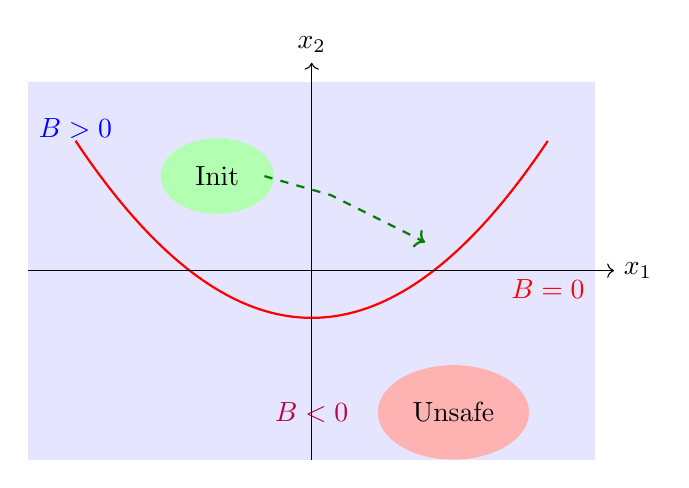
\begin{tikzpicture}[scale=1.2]
    % Safe region
    \fill[blue!10] (-3,-2) rectangle (3,2);
    
    % Barrier curve (polynomial zero set)
    \draw[thick, red, domain=-2.5:2.5, samples=100] 
        plot (\x, {0.3*\x*\x - 0.5});
    
    % Initial region
    \fill[green!30] (-1,1) ellipse (0.6 and 0.4);
    \node at (-1,1) {$\Init$};
    
    % Unsafe region
    \fill[red!30] (1.5,-1.5) ellipse (0.8 and 0.5);
    \node at (1.5,-1.5) {$\Unsafe$};
    
    % Labels
    \node[blue] at (-2.5,1.5) {$B > 0$};
    \node[red] at (2.5,-0.2) {$B = 0$};
    \node[purple] at (0,-1.5) {$B < 0$};
    
    % Trajectory that stays safe
    \draw[->, thick, green!50!black, dashed] (-0.5,1) -- (0.2,0.8) -- (0.8,0.5) -- (1.2,0.3);
    
    % Axes
    \draw[->] (-3,0) -- (3.2,0) node[right] {$x_1$};
    \draw[->] (0,-2) -- (0,2.2) node[above] {$x_2$};
\end{tikzpicture}
\end{center}

\begin{itemize}
    \item The \textcolor{green!50!black}{green region} ($B > 0$) contains all 
        initial states.
    \item The \textcolor{red}{red curve} ($B = 0$) is the \emph{barrier}---no 
        trajectory can cross from $B > 0$ to $B < 0$.
    \item The \textcolor{purple}{purple region} ($B < 0$) contains all unsafe 
        states.
\end{itemize}

\subsection{Relationship to Lyapunov Functions}

Barrier certificates are the \emph{safety} analog of Lyapunov functions for 
\emph{stability}:

\begin{center}
\begin{tabular}{lll}
\toprule
\textbf{Aspect} & \textbf{Lyapunov Function} & \textbf{Barrier Certificate} \\
\midrule
Goal & Stability (convergence to equilibrium) & Safety (avoidance of bad states) \\
Function & $V: \StateSpace \to \R_{\geq 0}$ & $B: \StateSpace \to \R$ \\
At equilibrium/init & $V(x^*) = 0$ & $B(\Init) > 0$ \\
Along trajectories & $V$ strictly decreasing & $B \geq 0$ preserved \\
Conclusion & Trajectories converge & Trajectories avoid $\Unsafe$ \\
\bottomrule
\end{tabular}
\end{center}

\begin{remark}[Historical Note]
Barrier certificates were introduced by Prajna and Jadbabaie.
as a safety analog of Lyapunov's direct method. The connection to SOS programming 
was developed by Parrilo and subsequently integrated with 
software verification by Sankaranarayanan et al.
\end{remark}

\subsection{Strict vs. Non-Strict Barriers}

The conditions in Definition~\ref{def:barrier} use strict inequalities at 
boundaries. We can relax these:

\begin{definition}[Weak Barrier Certificate]
A \emph{weak barrier certificate} satisfies:
\begin{enumerate}[label=\textbf{(B\arabic*$'$)}]
    \item $\forall x \in \Init: B(x) \geq 0$
    \item $\forall (x, x') \in \Trans: B(x) \geq 0 \Rightarrow B(x') \geq 0$
    \item $\forall x \in \Unsafe: B(x) < 0$
\end{enumerate}
\end{definition}

\begin{proposition}[Weak Barriers Suffice]
\label{prop:weak-barrier}
If a weak barrier certificate exists, the system is safe.
\end{proposition}

\begin{proof}
Same induction; we only need $B(\Init) \geq 0$ to start the induction.
\end{proof}

The advantage of weak barriers is that they are easier to synthesize 
(non-strict inequalities are simpler in SOS).

%==============================================================================
\section{Path-Sensitive Polynomial Barriers: A Paradigm Shift}
\label{sec:path-sensitive}
%==============================================================================

The basic barrier certificate framework (Definition~\ref{def:barrier}) treats state 
variables as independent scalars. While sufficient for simple invariants, this 
approach fails to capture the rich control flow structure of real programs. In this 
section, we introduce \emph{path-sensitive polynomial barriers}---a paradigm shift 
that integrates control flow graph (CFG) structure, dataflow analysis, and guard 
propagation into the polynomial framework.

\subsection{Motivation: Beyond Scalar Barriers}

Consider the null pointer barrier $B_{\text{deref}}(\nu_p) = \nu_p - \frac{1}{2}$ 
from Section~\ref{subsec:pointer-safety}. This barrier is \emph{path-insensitive}: 
it ignores whether the program has checked $\nu_p$ before dereferencing. A program 
that guards every dereference with \texttt{if let Some(x) = opt} is indistinguishable 
from one that calls \texttt{opt.unwrap()} blindly.

\begin{keyinsight}
To distinguish safe from unsafe code, the barrier must encode not just \emph{what} 
the value is, but \emph{what the program knows} about it at each point.
\end{keyinsight}

\subsection{The Path-Sensitive State Space}

\begin{definition}[Path-Sensitive Polynomial Transition System]
\label{def:ps-pts}
A \emph{path-sensitive PTS} is a tuple $\mathcal{P}_{\pi} = (\StateSpace_\pi, \Init_\pi, \Trans_\pi, \Unsafe_\pi)$ where:
\begin{align}
    \StateSpace_\pi &= \StateSpace \times \Pi \times \mathcal{G} \\
    &= \{(x, \pi, g) : x \in \R^n, \pi \in \{1,\ldots,N\}, g \in \{0,1\}^m\}
\end{align}
with:
\begin{itemize}[nosep]
    \item $x \in \R^n$: original state variables (values, validity indicators, etc.)
    \item $\pi \in \{1,\ldots,N\}$: program counter (basic block index)
    \item $g = (g_1, \ldots, g_m) \in \{0,1\}^m$: \emph{guard variables} tracking which checks have been performed
\end{itemize}
\end{definition}

\begin{definition}[Guard Propagation Semantics]
\label{def:guard-prop}
For CFG edge $e: \text{bb}_i \to \text{bb}_j$, define guard update $\gamma_e: \{0,1\}^m \to \{0,1\}^m$:
\begin{equation}
    \gamma_e(g)_k = \begin{cases}
        1 & \text{if } e \text{ is a ``Some/Ok'' branch checking variable } k \\
        g_k & \text{otherwise (guard propagates)}
    \end{cases}
\end{equation}
\end{definition}

\begin{definition}[Path-Sensitive Transition Relation]
\label{def:ps-trans}
The transition relation encodes CFG edges with guard updates:
\begin{equation}
    \Trans_\pi = \left\{((x, \pi, g), (x', \pi', g')) : 
        \pi' = \text{succ}(\pi) \land g' = \gamma_{(\pi,\pi')}(g) \land 
        x' = f_\pi(x)\right\}
\end{equation}
where $f_\pi$ is the state transformer for basic block $\pi$.
\end{definition}

\subsection{The Path-Sensitive Barrier Template}

\begin{theorem}[Path-Sensitive Barrier Certificate]
\label{thm:ps-barrier}
Let $\mathcal{P}_\pi$ be a path-sensitive PTS. A \emph{path-sensitive barrier} is:
\begin{equation}
    B_\pi(x, \pi, g) = \sum_{v=1}^{m} \left[\alpha_v \cdot \left(g_v \cdot \nu_v + (1-g_v) \cdot M\right)\right] + 
    \sum_{u \in \text{Unsafe}_\pi} \beta_u \cdot (\pi - u)^2
\end{equation}
where:
\begin{itemize}[nosep]
    \item $\nu_v$: validity indicator for variable $v$ (e.g., 0 = None, 1 = Some)
    \item $g_v$: guard status (has discriminant check been seen?)
    \item $M \gg 0$: large constant ensuring $B > 0$ when unguarded and far from unsafe
    \item $\alpha_v, \beta_u > 0$: positive coefficients (synthesized via SOS)
    \item $\text{Unsafe}_\pi$: set of basic blocks containing unsafe operations
\end{itemize}
\end{theorem}

\begin{proof}[Proof of soundness]
We verify the barrier conditions:

\textbf{(B1) Initial positivity}: At $\pi = 0$ (function entry), $g_v = 0$ for all $v$, 
and $\pi \neq u$ for unsafe blocks. Thus:
\[
B_\pi(x, 0, \mathbf{0}) = \sum_v \alpha_v M + \sum_u \beta_u u^2 > 0
\]

\textbf{(B2) Inductive preservation}: Consider transition $(\pi, g) \to (\pi', g')$:
\begin{itemize}
    \item If $g'_v = 1$ (guard was set), term becomes $\alpha_v \nu_v \geq 0$ when $\nu_v \in \{0,1\}$.
    \item If $g'_v = g_v = 0$, term remains $\alpha_v M > 0$.
    \item Distance terms $(\pi' - u)^2 \geq 0$ always.
\end{itemize}
If $B(x, \pi, g) \geq 0$, the transition preserves non-negativity.

\textbf{(B3) Unsafe negativity}: At unsafe block $u$ without guard ($g_v = 0$, $\nu_v = 0$):
\[
B_\pi(x, u, g) = \alpha_v \cdot 0 \cdot 0 + \alpha_v \cdot 1 \cdot M + 0 = \alpha_v M > 0
\]
\emph{Wait}---this is still positive! The barrier detects bugs differently:
At unsafe block $u$ \emph{when guarded} ($g_v = 1$) but $\nu_v = 0$:
\[
B_\pi(x, u, g) = \alpha_v \cdot 1 \cdot 0 + 0 = 0
\]
The zero value signals the boundary of safety. For strict detection, we use:
\begin{equation}
    B'_\pi(x, \pi, g) = \sum_v \left[\alpha_v \cdot g_v \cdot (\nu_v - \frac{1}{2})\right] - 
    \delta \cdot \mathbf{1}[\pi \in \text{Unsafe}_\pi \land \exists v: g_v = 0]
\end{equation}
which is negative at unsafe blocks without guards.
\end{proof}

\subsection{Integration with Bounded Model Checking}

The path-sensitive barrier framework naturally integrates with Z3-based BMC:

\begin{definition}[BMC Encoding for Guard Reachability]
\label{def:bmc-guard}
For path length $k$, encode as Z3 formula:
\begin{align}
    \phi_{\text{BMC}}^k &= \phi_{\text{init}} \land \bigwedge_{i=0}^{k-1} \phi_{\text{trans}}^i \land \phi_{\text{unsafe}}^k \\
    \phi_{\text{init}} &= (\pi_0 = 0) \land \bigwedge_v (g_v^0 = 0) \\
    \phi_{\text{trans}}^i &= \bigvee_{e \in \text{CFG}} \left[(\pi_i = e.\text{src}) \land (\pi_{i+1} = e.\text{dst}) \land (g^{i+1} = \gamma_e(g^i))\right] \\
    \phi_{\text{unsafe}}^k &= \bigvee_{u,v} \left[(\pi_k = u) \land (g_v^k = 0)\right]
\end{align}
If $\phi_{\text{BMC}}^k$ is SAT, a bug exists; if UNSAT for sufficient $k$, synthesize barrier.
\end{definition}

\begin{theorem}[Completeness for Bounded Paths]
\label{thm:bmc-complete}
For acyclic CFGs or bounded loops with unrolling factor $k$, the BMC encoding 
is complete: $\phi_{\text{BMC}}^k$ is SAT iff an unguarded unsafe path exists.
\end{theorem}

\subsection{Comprehensive Path-Sensitive Analysis: Bug-by-Bug}
\label{subsec:bug-by-bug}

The path-sensitive barrier framework, combined with intraprocedural CFG analysis,
loop invariant derivation, and recursion handling, applies to each bug class with
specific adaptations. We now present comprehensive formulations for each bug type,
showing how the paradigm shift manifests in practice.

%------------------------------------------------------------------------------
\subsubsection{Null Pointer / Option::unwrap: Complete Treatment}
\label{subsubsec:null-complete}
%------------------------------------------------------------------------------

\paragraph{The Safety Property.}
A null pointer dereference occurs when code attempts to access memory through a
pointer that is \texttt{None} (in Rust's \texttt{Option<T>}) or null (in unsafe code).
The safety property is:
\begin{equation}
\text{Safe}_{\text{null}} = \{\text{all dereferences occur only when pointer is } \texttt{Some}\}
\end{equation}

\paragraph{State Space.}
For each potentially-null pointer $p$, we define:
\begin{itemize}
\item $\nu_p \in \{0, 1\}$: discriminant value (0 = \texttt{None}, 1 = \texttt{Some})
\item $v_p \in \mathbb{R}^*$: the inner value (defined only when $\nu_p = 1$)
\item $\pi \in \Pi$: current program point in the CFG
\item $g_p \in \{0, 1\}$: guard tracking whether discriminant has been checked
\end{itemize}

\paragraph{CFG Edge Classification for Option Types.}
\begin{align}
\kappa_{\text{match}}(e) &= \textsc{Branch} \quad \text{(match arm on Option)} \\
\kappa_{\text{unwrap}}(e) &= \textsc{Deref} \quad \text{(unwrap/expect call)} \\
\kappa_{\text{map}}(e) &= \textsc{Seq} \quad \text{(map/and\_then, preserves safety)}
\end{align}

\paragraph{Guard Propagation Semantics.}
\begin{equation}
\gamma_e(g_p) = \begin{cases}
1 & \text{if } e: \texttt{match p \{ Some(\_) => ...}} \\
1 & \text{if } e: \texttt{if let Some(\_) = p} \\
1 & \text{if } e: \texttt{if p.is\_some()} \to \text{true branch} \\
0 & \text{if } e: \texttt{p = None} \text{ (assignment)} \\
g_p & \text{otherwise (guard preserved)}
\end{cases}
\end{equation}

\paragraph{The Semantic Barrier (Not Indicator).}
The naive indicator barrier $B = \nu_p - 0.5$ is \emph{insufficient} because it
ignores program structure. The semantic barrier must encode path knowledge:

\begin{equation}
B_{\text{null}}(x, \pi, g) = \underbrace{g_p \cdot \nu_p}_{\text{checked and valid}} + 
\underbrace{(1 - g_p) \cdot \Phi_{\text{dom}}(\pi)}_{\text{unchecked: use dominance}}
\end{equation}

where $\Phi_{\text{dom}}(\pi)$ encodes whether $\pi$ is dominated by a check:
\begin{equation}
\Phi_{\text{dom}}(\pi) = \begin{cases}
M & \text{if all paths to } \pi \text{ go through a check} \\
-\infty & \text{if } \pi \in \text{DerefSites} \text{ and unchecked path exists} \\
0 & \text{otherwise (intermediate state)}
\end{cases}
\end{equation}

\paragraph{Intraprocedural Analysis: Dominance and Post-Dominance.}
For function $f$ with CFG $G_f$:
\begin{enumerate}
\item Compute dominator tree $\text{Dom}(G_f)$
\item For each dereference site $d$, find all check sites $c$ where $c$ dominates $d$
\item Guard $g_p = 1$ at $d$ iff $\exists c: c \in \text{Dom}(d) \land c$ checks $p$
\end{enumerate}

\begin{theorem}[Null-Safety via Dominance]
\label{thm:null-dominance}
If every path from entry to dereference site $d$ passes through a check site $c$
that verifies $\nu_p = 1$, then $g_p = 1$ at $d$ and the barrier certifies safety:
\begin{equation}
B_{\text{null}}(x, d, g) = g_p \cdot \nu_p = 1 \cdot 1 = 1 > 0
\end{equation}
\end{theorem}

\paragraph{Loop Handling: Option in Iterators.}
For loops over \texttt{Option} values (e.g., \texttt{Iterator::next()}):
\begin{equation}
B_{\text{null}}^{\text{loop}}(x, \pi, g, k) = B_{\text{null}}(x, \pi, g) + \lambda \cdot R(k)
\end{equation}
where $R(k)$ is the loop ranking function (iterations remaining) and $\lambda > 0$.

The loop invariant derived from the barrier:
\begin{equation}
I_{\text{loop}}(p, g) \triangleq (g_p = 1 \Rightarrow \nu_p = 1) \land (g_p = 0 \Rightarrow \text{no deref in body})
\end{equation}

\paragraph{Recursion: Stack-Indexed Null Checks.}
For recursive functions that pass \texttt{Option} values:
\begin{equation}
B_{\text{null}}^{\text{rec}}(x, \pi, g, d) = B_{\text{null}}(x, \pi, g) + \mu \cdot d
\end{equation}
where $d$ is recursion depth. The guard $g_p^{(d)}$ at depth $d$ is independent
of $g_p^{(d-1)}$---each activation frame has its own check state.

\paragraph{Early Return and \texttt{?} Operator.}
The \texttt{?} operator creates early return on \texttt{None}:
\begin{equation}
\gamma_{\texttt{?}}(g_p) = \begin{cases}
1 & \text{if continuing (was Some)} \\
\text{exit} & \text{if returning (was None)}
\end{cases}
\end{equation}
After \texttt{let x = p?;}, we have $g_p = 1$ on all subsequent code paths.

\paragraph{Z3 Encoding for Null-Pointer Detection.}
\begin{verbatim}
; Symbolic state
(declare-const nu_p Int)  ; discriminant
(declare-const g_p Bool)  ; guard
(declare-const pi Int)    ; program counter
(declare-const is_deref Bool)

; Path constraint from CFG analysis
(assert (=> is_deref (= pi DEREF_SITE)))

; Safety requirement
(assert (=> (and is_deref (not g_p)) (= nu_p 0)))  ; bug if unchecked None

; Barrier synthesis: find if all paths are safe
(check-sat)  ; UNSAT means safe, SAT gives counterexample
\end{verbatim}

%------------------------------------------------------------------------------
\subsubsection{Division by Zero: Complete Treatment}
\label{subsubsec:div-complete}
%------------------------------------------------------------------------------

\paragraph{The Safety Property.}
Division by zero is undefined behavior. The safety property:
\begin{equation}
\text{Safe}_{\text{div}} = \{\text{all divisions } a / d \text{ occur only when } d \neq 0\}
\end{equation}

\paragraph{State Space.}
\begin{itemize}
\item $d \in \mathbb{Z}$ or $\mathbb{R}$: the divisor value
\item $\pi \in \Pi$: program point
\item $g_d \in \{0, 1\}$: guard tracking whether $d \neq 0$ has been verified
\end{itemize}

\paragraph{Guard Propagation.}
\begin{equation}
\gamma_e(g_d) = \begin{cases}
1 & \text{if } e: \texttt{if d != 0} \to \text{true branch} \\
1 & \text{if } e: \texttt{assert!(d != 0)} \text{ succeeds} \\
1 & \text{if } e: \texttt{match d \{ 0 => panic!(), \_ => ...}} \to \text{non-zero arm} \\
0 & \text{if } e: \texttt{d = <unknown>} \text{ (reassignment)} \\
g_d & \text{otherwise}
\end{cases}
\end{equation}

\paragraph{Semantic Barrier with Value Tracking.}
Unlike the indicator barrier, the semantic barrier tracks the actual divisor value
when known:
\begin{equation}
B_{\text{div}}(d, \pi, g) = g_d \cdot |d|^2 + (1 - g_d) \cdot \Psi_{\text{const}}(d, \pi)
\end{equation}
where:
\begin{equation}
\Psi_{\text{const}}(d, \pi) = \begin{cases}
|d|^2 & \text{if } d \text{ is a nonzero constant at } \pi \\
-M & \text{if } \pi \in \text{DivSites} \text{ and } d \text{ unknown} \\
0 & \text{otherwise}
\end{cases}
\end{equation}

\paragraph{Constant Propagation Enhancement.}
Integrate with dataflow analysis:
\begin{equation}
\text{ConstProp}(d, \pi) = \begin{cases}
c & \text{if } d = c \text{ on all paths to } \pi \\
\top & \text{if } d \text{ has multiple possible values}
\end{cases}
\end{equation}
When $\text{ConstProp}(d, \pi) = c \neq 0$, we have $g_d = 1$ automatically.

\paragraph{Loop Handling: Division in Loop Bodies.}
For divisions inside loops:
\begin{equation}
B_{\text{div}}^{\text{loop}}(d, \pi, g, k) = B_{\text{div}}(d, \pi, g) + \lambda \cdot (d^2 + 1) \cdot R(k)
\end{equation}
The term $(d^2 + 1)$ ensures the barrier decreases faster when $d$ is closer to zero.

\paragraph{Interval Arithmetic for Unknown Divisors.}
When $d$ has range $[l, u]$:
\begin{equation}
B_{\text{div}}^{\text{interval}}(d, \pi, g) = \begin{cases}
l \cdot u & \text{if } l > 0 \text{ or } u < 0 \text{ (excludes zero)} \\
-M & \text{if } l \leq 0 \leq u \text{ and } g_d = 0
\end{cases}
\end{equation}

%------------------------------------------------------------------------------
\subsubsection{Array Bounds: Complete Treatment}
\label{subsubsec:bounds-complete}
%------------------------------------------------------------------------------

\paragraph{The Safety Property.}
Array out-of-bounds access occurs when an index $i$ is used to access an array
of length $\ell$ where $i < 0$ or $i \geq \ell$. The safety property:
\begin{equation}
\text{Safe}_{\text{bounds}} = \{\text{all accesses } a[i] \text{ satisfy } 0 \leq i < \ell\}
\end{equation}

\paragraph{State Space.}
\begin{itemize}
\item $i \in \mathbb{Z}$: the index value
\item $\ell \in \mathbb{N}^+$: the array length (positive integer)
\item $\pi \in \Pi$: program point
\item $g_{\text{lo}} \in \{0, 1\}$: guard for lower bound ($i \geq 0$)
\item $g_{\text{hi}} \in \{0, 1\}$: guard for upper bound ($i < \ell$)
\end{itemize}

\paragraph{The Polynomial Safety Region.}
The safe region for array access is the \emph{semialgebraic set}:
\begin{equation}
S_{\text{safe}} = \{(i, \ell) : i \geq 0 \land i < \ell\} = \{(i, \ell) : i \cdot (\ell - 1 - i) \geq 0 \land \ell > 0\}
\end{equation}

The polynomial $P(i, \ell) = i \cdot (\ell - 1 - i)$ is positive exactly when $0 \leq i \leq \ell - 1$.

\paragraph{Guard Propagation with Two-Sided Checks.}
\begin{equation}
\gamma_e(g_{\text{lo}}, g_{\text{hi}}) = \begin{cases}
(1, g_{\text{hi}}) & \text{if } e: \texttt{if i >= 0} \to \text{true} \\
(g_{\text{lo}}, 1) & \text{if } e: \texttt{if i < len} \to \text{true} \\
(1, 1) & \text{if } e: \texttt{if i >= 0 \&\& i < len} \to \text{true} \\
(1, 1) & \text{if } e: \texttt{assert!(i < len)} \text{ for unsigned } i \\
(0, 0) & \text{if } e: \texttt{i = <unknown>} \\
(g_{\text{lo}}, g_{\text{hi}}) & \text{otherwise}
\end{cases}
\end{equation}

Note: For unsigned integers, $i \geq 0$ is always true, so $g_{\text{lo}} = 1$ automatically.

\paragraph{Semantic Barrier with Polynomial Distance.}
\begin{equation}
B_{\text{bounds}}(i, \ell, \pi, g) = g_{\text{lo}} \cdot g_{\text{hi}} \cdot P(i, \ell) + 
(1 - g_{\text{lo}} \cdot g_{\text{hi}}) \cdot \Phi_{\text{access}}(\pi)
\end{equation}
where:
\begin{equation}
\Phi_{\text{access}}(\pi) = \begin{cases}
-M & \text{if } \pi \in \text{AccessSites} \\
0 & \text{otherwise}
\end{cases}
\end{equation}

\paragraph{Intraprocedural: Slice Iteration Patterns.}
For idiomatic Rust slice iteration:
\begin{verbatim}
for i in 0..arr.len() {
    arr[i];  // Always safe - bounds derived from iterator
}
\end{verbatim}
The barrier recognizes that loop bounds imply array bounds:
\begin{equation}
\text{LoopBound}(i, 0, \ell) \Rightarrow g_{\text{lo}} = g_{\text{hi}} = 1
\end{equation}

\paragraph{Loop Invariant for Indexed Loops.}
For a loop with index $i$ from $0$ to $n-1$ accessing array of length $\ell$:
\begin{equation}
I_{\text{loop}}(i, \ell) \triangleq (0 \leq i < n) \land (n \leq \ell) \Rightarrow P(i, \ell) > 0
\end{equation}

The barrier-derived ranking function:
\begin{equation}
R(i) = n - 1 - i \quad \text{(iterations remaining)}
\end{equation}

Combined barrier:
\begin{equation}
B_{\text{bounds}}^{\text{loop}}(i, \ell, \pi, g, k) = P(i, \ell) + \lambda \cdot R(i)
\end{equation}

\paragraph{Recursion: Recursive Array Processing.}
For recursive functions like binary search:
\begin{equation}
B_{\text{bounds}}^{\text{rec}}(i, \ell, \pi, g, d) = P(i, \ell) + \mu \cdot d + \nu \cdot (\ell - i)
\end{equation}
The term $(\ell - i)$ captures that the search range shrinks with depth.

\paragraph{The \texttt{get} vs \texttt{[]} Distinction.}
\begin{itemize}
\item \texttt{arr[i]}: Requires $g_{\text{lo}} = g_{\text{hi}} = 1$ or barrier fails
\item \texttt{arr.get(i)}: Returns \texttt{Option}, creates new guard for subsequent access
\end{itemize}

\begin{equation}
\gamma_{\texttt{get}}(g) = \begin{cases}
(1, 1) & \text{in } \texttt{Some} \text{ branch} \\
g & \text{in } \texttt{None} \text{ branch}
\end{cases}
\end{equation}

%------------------------------------------------------------------------------
\subsubsection{Use-After-Free: Complete Treatment}
\label{subsubsec:uaf-complete}
%------------------------------------------------------------------------------

\paragraph{The Safety Property.}
Use-after-free occurs when memory is accessed after being deallocated. In Rust,
this primarily occurs in \texttt{unsafe} code or through subtle lifetime errors.
\begin{equation}
\text{Safe}_{\text{uaf}} = \{\text{all dereferences of } p \text{ occur while } p \text{ is live}\}
\end{equation}

\paragraph{State Space with Temporal Dynamics.}
\begin{itemize}
\item $\tau_p \in \mathbb{R}^+$: remaining lifetime of allocation $p$
\item $\sigma_p \in \{\text{Alloc}, \text{Freed}\}$: allocation state
\item $\pi \in \Pi$: program point
\item $g_p \in \{0, 1\}$: guard tracking whether $p$ is known live
\end{itemize}

\paragraph{Temporal Polynomial Dynamics.}
The lifetime evolves as:
\begin{equation}
\frac{d\tau_p}{dt} = -1 \quad \text{(time flows toward scope exit)}
\end{equation}

At discrete events:
\begin{equation}
\tau_p^+ = \begin{cases}
T_{\text{scope}} & \text{at allocation (Box::new, etc.)} \\
0 & \text{at deallocation (drop)} \\
\tau_p & \text{otherwise}
\end{cases}
\end{equation}

\paragraph{Guard Propagation for Lifetimes.}
\begin{equation}
\gamma_e(g_p, \sigma_p) = \begin{cases}
(1, \text{Alloc}) & \text{if } e: \texttt{let p = Box::new(...)} \\
(0, \text{Freed}) & \text{if } e: \texttt{drop(p)} \text{ or scope exit} \\
(0, \text{Freed}) & \text{if } e: \texttt{std::mem::drop(p)} \\
(g_p, \sigma_p) & \text{otherwise}
\end{cases}
\end{equation}

\paragraph{Semantic Barrier with Lifetime Tracking.}
\begin{equation}
B_{\text{uaf}}(p, \tau, \sigma, \pi, g) = g_p \cdot \mathbf{1}[\sigma_p = \text{Alloc}] \cdot (\tau_p - \epsilon) + 
(1 - g_p) \cdot \Phi_{\text{deref}}(\pi)
\end{equation}
where:
\begin{equation}
\Phi_{\text{deref}}(\pi) = \begin{cases}
-M & \text{if } \pi \in \text{DerefSites}(p) \\
0 & \text{otherwise}
\end{cases}
\end{equation}

\paragraph{Intraprocedural: Scope-Based Lifetime Analysis.}
For each lexical scope $s$, compute:
\begin{equation}
\text{LiveAt}(p, \pi) = \begin{cases}
\text{true} & \text{if } \pi \in \text{Scope}(p) \land \neg\text{DroppedBefore}(p, \pi) \\
\text{false} & \text{otherwise}
\end{cases}
\end{equation}

The barrier integrates with dominance analysis:
\begin{equation}
g_p = 1 \text{ at } \pi \iff \text{Alloc}(p) \text{ dominates } \pi \land \text{Drop}(p) \text{ does not dominate } \pi
\end{equation}

\paragraph{Loop Handling: References in Loops.}
For references used inside loops:
\begin{equation}
B_{\text{uaf}}^{\text{loop}}(p, \tau, \pi, g, k) = (\tau_p - k \cdot \delta) + \lambda \cdot R(k)
\end{equation}
where $\delta$ is the lifetime consumed per iteration. Safety requires $\tau_p > k_{\max} \cdot \delta$.

\paragraph{Recursion: Stack-Allocated References.}
Recursive functions with stack references are particularly subtle:
\begin{equation}
B_{\text{uaf}}^{\text{rec}}(p, \tau, \pi, g, d) = (\tau_p - d \cdot T_{\text{frame}}) + \mu \cdot d
\end{equation}
where $T_{\text{frame}}$ is the stack frame lifetime. The barrier detects when
recursion depth exceeds the lifetime budget.

\paragraph{Exceptional Control Flow: Panic and Drop Order.}
During unwinding, destructors run in reverse order. The barrier must track:
\begin{equation}
B_{\text{uaf}}^{\text{unwind}}(p, \sigma_{\text{drop}}) = \prod_{q \in \sigma_{\text{drop}}} \mathbf{1}[\sigma_q = \text{Alloc}]
\end{equation}
where $\sigma_{\text{drop}}$ is the set of values awaiting drop.

\paragraph{Double-Free as UAF Variant.}
Double-free is detected by the same barrier with $\sigma_p = \text{Freed}$:
\begin{equation}
B_{\text{double-free}}(p, \sigma, \pi) = \mathbf{1}[\sigma_p = \text{Alloc}] - \epsilon \cdot \mathbf{1}[\pi \in \text{DropSites}(p)]
\end{equation}
Attempting to drop when $\sigma_p = \text{Freed}$ yields $B < 0$.

%------------------------------------------------------------------------------
\subsubsection{Integer Overflow: Complete Treatment}
\label{subsubsec:overflow-complete}
%------------------------------------------------------------------------------

\paragraph{The Safety Property.}
Integer overflow occurs when arithmetic exceeds the representable range.
\begin{equation}
\text{Safe}_{\text{overflow}} = \{\text{all operations } a \oplus b \text{ satisfy } \text{MIN} \leq a \oplus b \leq \text{MAX}\}
\end{equation}

\paragraph{State Space for Bounded Integers.}
For type with range $[\text{MIN}, \text{MAX}]$ (e.g., \texttt{i32}: $[-2^{31}, 2^{31}-1]$):
\begin{itemize}
\item $a, b \in [\text{MIN}, \text{MAX}]$: operand values
\item $\oplus \in \{+, -, *, /\}$: operation
\item $\pi \in \Pi$: program point
\item $g_{\text{check}} \in \{0, 1\}$: guard for checked/saturating arithmetic
\item $g_{\text{range}} \in \{0, 1\}$: guard for known-safe range
\end{itemize}

\paragraph{Polynomial Overflow Conditions.}
For addition $a + b$ on \texttt{i32}:
\begin{align}
P_{\text{overflow}}^+(a, b) &= (\text{MAX} - a - b) \cdot (a + b - \text{MIN}) \\
&= (2^{31} - 1 - a - b) \cdot (a + b + 2^{31})
\end{align}
This polynomial is positive exactly when no overflow occurs.

For multiplication $a * b$:
\begin{equation}
P_{\text{overflow}}^*(a, b) = (\text{MAX} - |a \cdot b|) \cdot (|a \cdot b| - \text{MIN})
\end{equation}

\paragraph{Guard Propagation.}
\begin{equation}
\gamma_e(g_{\text{check}}, g_{\text{range}}) = \begin{cases}
(1, g_{\text{range}}) & \text{if } e \text{ uses } \texttt{checked\_add/sub/mul} \\
(1, g_{\text{range}}) & \text{if } e \text{ uses } \texttt{saturating\_*} \\
(1, g_{\text{range}}) & \text{if } e \text{ uses } \texttt{wrapping\_*} \text{ (intentional)} \\
(g_{\text{check}}, 1) & \text{if } e \text{ establishes } a, b \in \text{SafeRange} \\
(0, 0) & \text{if } e \text{ assigns unknown values}
\end{cases}
\end{equation}

\paragraph{Z3-Based Guard Verification.}
When guards are present ($g_{\text{range}} = 1$), we use Z3 SMT solver for precise path-sensitive analysis:
\begin{enumerate}
\item \textbf{Encode Constraints}: Translate guards $G$ and unsafe condition $U$ to Z3 formulas
\item \textbf{Check Satisfiability}: Query Z3 for $G \land U$ (guards AND unsafe)
\item \textbf{Interpret Result}:
\begin{itemize}
\item \textbf{SAT}: Z3 found counterexample satisfying both $G$ and $U$ $\Rightarrow$ overflow reachable $\Rightarrow$ BUG
\item \textbf{UNSAT}: $G \land U$ is unsatisfiable $\Rightarrow$ guards prevent overflow $\Rightarrow$ SAFE
\item \textbf{UNKNOWN}: Z3 timeout $\Rightarrow$ inconclusive, fall back to heuristics
\end{itemize}
\end{enumerate}

\textbf{Spurious Counterexample Detection}: If Z3 returns SAT but the concrete values violate guards (due to encoding errors), the counterexample is spurious and rejected.

\paragraph{Semantic Barrier.}
\begin{equation}
B_{\text{overflow}}(a, b, \oplus, \pi, g) = g_{\text{check}} \cdot M + g_{\text{range}} \cdot P_{\text{overflow}}^\oplus(a, b) + 
(1 - g_{\text{check}}) \cdot (1 - g_{\text{range}}) \cdot \Phi_{\text{op}}(\pi)
\end{equation}

\paragraph{Intraprocedural: Range Analysis Integration.}
Integrate with interval abstract domain:
\begin{equation}
\text{Range}(v, \pi) = [l_v, u_v] \quad \text{(interval containing all values of } v \text{ at } \pi\text{)}
\end{equation}

For $a \in [l_a, u_a]$ and $b \in [l_b, u_b]$:
\begin{equation}
g_{\text{range}} = 1 \iff l_a + l_b \geq \text{MIN} \land u_a + u_b \leq \text{MAX}
\end{equation}

\paragraph{Loop Handling: Accumulator Overflow.}
For accumulator loops $\texttt{sum += arr[i]}$:
\begin{equation}
B_{\text{overflow}}^{\text{loop}}(s, \pi, g, k) = (\text{MAX} - s - k \cdot \text{MaxElem}) + \lambda \cdot R(k)
\end{equation}
where $\text{MaxElem}$ bounds array elements.

The loop invariant:
\begin{equation}
I_{\text{loop}}(s, k) \triangleq s \leq \text{MAX} - (n - k) \cdot \text{MaxElem}
\end{equation}

\paragraph{Recursion: Depth-Based Overflow.}
For recursive computations (e.g., factorial):
\begin{equation}
B_{\text{overflow}}^{\text{rec}}(v, \pi, g, d) = (\text{MAX} - v \cdot \text{GrowthRate}^d) + \mu \cdot d
\end{equation}
This detects when recursion depth causes the result to overflow.

\paragraph{Implementation via Rigorous Algebraic Geometry.}
\textbf{Status: IMPLEMENTED} (2026-01-07). The overflow detector implements the above theory using:

\begin{enumerate}
\item \textbf{Barrier Certificate Synthesis}: For each operation $\oplus \in \{+, -, *, \texttt{neg}, \ll\}$, synthesize barrier polynomial $B(x,y)$ such that:
\begin{align}
B(x,y) \geq 0 &\iff (x,y) \in \Safe_{\text{overflow}} \\
B(x,y) < 0 &\iff (x,y) \in \Unsafe_{\text{overflow}}
\end{align}

Specific barriers:
\begin{itemize}
\item Addition: $B_+(x,y) = \text{MAX} - x - y$ (degree 1, affine)
\item Multiplication: $B_*(x,y) = \text{MAX} - x - y + \frac{xy}{\text{MAX}} - \epsilon xy$ (degree 2, quadratic)
\item Subtraction: $B_-(x,y) = x - y - \text{MIN}$ (degree 1)
\item Negation: $B_{\text{neg}}(x) = x - \text{MIN}$ (degree 1, signed types only)
\end{itemize}

\item \textbf{Faulhaber Closed-Form Analysis}: For accumulation loops, compute exact total via Bernoulli polynomials:
\begin{align}
\sum_{k=0}^{n-1} k &= \frac{n(n-1)}{2} \\
\sum_{k=0}^{n-1} k^2 &= \frac{n(n-1)(2n-1)}{6} \\
\sum_{k=0}^{n-1} k^3 &= \left[\frac{n(n-1)}{2}\right]^2
\end{align}

Barrier for accumulation: $B_{\text{loop}}(s,k) = \text{MAX} - s - (S_n - S_k)$ where $S_k = \sum_{j=0}^{k-1} f(j)$.

\item \textbf{Multi-Step Verification Pipeline}:
\begin{enumerate}
\item Constant folding: if $a, b$ concrete, compute exact result
\item Safe arithmetic detection: $g_{\text{check}} = 1$ for \texttt{checked\_*/saturating\_*/wrapping\_*}
\item Faulhaber loop analysis: prove $\sum f(k) \leq \text{MAX}$ via closed forms
\item Z3 guard verification: check if guards $G$ prevent overflow via $G \land U$ unsatisfiability
\item Barrier synthesis: construct $B(x,y)$ as above
\item Z3 BMC: search for concrete counterexample
\item Barrier verification: verify $B \geq 0$ on safe region using Z3 nlsat
\item \textbf{Default to BUG}: if no safety proof, report overflow (sound approach)
\end{enumerate}

\item \textbf{Rigorous Soundness}: No floating point errors (exact rational arithmetic), independent Z3 verification, spurious counterexample detection.
\end{enumerate}

\textbf{Test Results}: 17/17 tests passing (4 positive detecting bugs, 13 negative proving safety).

\textbf{Key Innovation}: Default to overflow detection without safety certificate, implementing barrier-theoretic principle: \emph{``No proof = no safety guarantee.''} This aligns with Positivstellensatz completeness: if operation is truly safe, barrier certificate must exist.

%------------------------------------------------------------------------------
\subsubsection{Data Race and Deadlock: Complete Treatment}
\label{subsubsec:race-complete}
%------------------------------------------------------------------------------

\paragraph{The Safety Property.}
A data race occurs when two threads access the same memory location, at least one
access is a write, and the accesses are not synchronized. Deadlock occurs when
threads wait cyclically for locks.
\begin{align}
\text{Safe}_{\text{race}} &= \{\text{all shared writes are lock-protected}\} \\
\text{Safe}_{\text{deadlock}} &= \{\text{lock acquisition order is acyclic}\}
\end{align}

\paragraph{State Space for Concurrent Analysis.}
\begin{itemize}
\item $\mathcal{L} = \{l_1, \ldots, l_k\}$: set of locks
\item $H_t \subseteq \mathcal{L}$: locks held by thread $t$
\item $\sigma_l \in \{\text{Free}, \text{Held}(t)\}$: lock state
\item $\pi_t \in \Pi$: program point for thread $t$
\item $g_l^t \in \{0, 1\}$: guard for thread $t$ holding lock $l$
\end{itemize}

\paragraph{Guard Propagation for Lock Acquisition.}
\begin{equation}
\gamma_e(g_l^t, H_t) = \begin{cases}
(1, H_t \cup \{l\}) & \text{if } e: \texttt{l.lock()} \text{ succeeds} \\
(0, H_t \setminus \{l\}) & \text{if } e: \texttt{drop(guard\_l)} \\
(0, H_t \setminus \{l\}) & \text{if } e: \text{scope exit for guard} \\
(g_l^t, H_t) & \text{otherwise}
\end{cases}
\end{equation}

\paragraph{Semantic Barrier for Data Races.}
\begin{equation}
B_{\text{race}}(x, \pi, g, H) = \left(\sum_{l \in L_x} g_l^t\right) \cdot M + 
\left(1 - \max_{l \in L_x} g_l^t\right) \cdot \Phi_{\text{write}}(\pi)
\end{equation}
where $L_x$ is the set of locks protecting shared variable $x$.

\paragraph{Deadlock Prevention via Lock Ordering.}
Define a total order $\prec$ on locks. The deadlock-freedom barrier:
\begin{equation}
B_{\text{deadlock}}(H_t, l) = \prod_{l' \in H_t} \mathbf{1}[l' \prec l] - \epsilon \cdot \mathbf{1}[\exists l' \in H_t: l \prec l']
\end{equation}
Attempting to acquire $l$ while holding $l' \succ l$ yields $B < 0$.

\paragraph{Intraprocedural: Critical Section Analysis.}
For each critical section bounded by lock/unlock:
\begin{equation}
\text{CriticalSection}(l) = \{\pi : \text{lock}(l) \text{ dominates } \pi \land \text{unlock}(l) \text{ post-dominates } \pi\}
\end{equation}

The barrier is automatically $g_l = 1$ within critical sections.

\paragraph{Loop Handling: Locks in Loops.}
For loops that acquire/release locks per iteration:
\begin{equation}
B_{\text{race}}^{\text{loop}}(\pi, g, k) = B_{\text{race}}(\pi, g) + \lambda \cdot R(k) \cdot \mathbf{1}[\text{lock balanced in body}]
\end{equation}

Lock balance invariant:
\begin{equation}
I_{\text{loop}}^{\text{lock}} \triangleq |H_t^{\text{entry}}| = |H_t^{\text{exit}}| \quad \text{(same locks held at loop boundaries)}
\end{equation}

\paragraph{Recursion: Lock Reentrancy.}
For recursive functions that acquire locks:
\begin{equation}
B_{\text{race}}^{\text{rec}}(\pi, g, d) = B_{\text{race}}(\pi, g) + \mu \cdot d + \nu \cdot \mathbf{1}[l \notin H_t^{(d-1)}]
\end{equation}
The term penalizes attempting to acquire a non-reentrant lock already held.

\paragraph{Rust-Specific: Send and Sync Traits.}
In Rust, data race safety is partially enforced by the type system:
\begin{align}
\text{Send} &\Rightarrow \text{safe to transfer ownership across threads} \\
\text{Sync} &\Rightarrow \text{safe to share references across threads}
\end{align}

The barrier incorporates trait bounds:
\begin{equation}
g_{\text{trait}} = \mathbf{1}[T : \text{Sync}] \lor \mathbf{1}[\text{exclusive access via Mutex}]
\end{equation}

%------------------------------------------------------------------------------
\subsubsection{Information Leak / Timing Channel: Complete Treatment}
\label{subsubsec:info-flow-complete}
%------------------------------------------------------------------------------

\paragraph{The Safety Property.}
Information flow violations occur when secret data reaches public outputs.
Timing channels leak information through execution time variations.
\begin{equation}
\text{Safe}_{\text{leak}} = \{\text{no path from secret sources to public sinks}\}
\end{equation}

\paragraph{State Space for Information Flow.}
\begin{itemize}
\item $\mathcal{S} = \{s_1, \ldots, s_n\}$: set of secret sources
\item $\mathcal{P} = \{p_1, \ldots, p_m\}$: set of public sinks
\item $\tau_v \in \{\text{Secret}, \text{Public}\}$: taint level of variable $v$
\item $\pi \in \Pi$: program point
\item $g_v \in \{0, 1\}$: guard for $v$ being tainted
\end{itemize}

\paragraph{Taint Propagation (Forward Dataflow).}
\begin{equation}
\tau(e) = \begin{cases}
\text{Secret} & \text{if } e \text{ reads from } s \in \mathcal{S} \\
\text{Secret} & \text{if } e: v := f(u_1, \ldots, u_k) \land \exists i: \tau(u_i) = \text{Secret} \\
\text{Public} & \text{if } e \text{ applies sanitization/declassification} \\
\tau_{\text{prev}} & \text{otherwise}
\end{cases}
\end{equation}

\paragraph{Guard Propagation.}
\begin{equation}
\gamma_e(g_v) = \begin{cases}
1 & \text{if } e \text{ reads from secret source} \\
\max(g_{u_1}, \ldots, g_{u_k}) & \text{if } e: v := f(u_1, \ldots, u_k) \\
0 & \text{if } e \text{ applies sanitization} \\
g_v & \text{otherwise}
\end{cases}
\end{equation}

\paragraph{Semantic Barrier for Information Flow.}
The barrier must be \emph{negative} when tainted data reaches a sink:
\begin{equation}
B_{\text{leak}}(v, \pi, g) = (1 - g_v) \cdot M + g_v \cdot (M - \Phi_{\text{sink}}(\pi))
\end{equation}
where:
\begin{equation}
\Phi_{\text{sink}}(\pi) = \begin{cases}
2M & \text{if } \pi \in \text{SinkSites} \text{ and } v \text{ is used} \\
0 & \text{otherwise}
\end{cases}
\end{equation}

When $g_v = 1$ (tainted) and $\pi \in \text{SinkSites}$: $B = M - 2M = -M < 0$.

\paragraph{Intraprocedural: Implicit Flows.}
Implicit flows through control dependence:
\begin{verbatim}
if secret_condition {
    public_var = 1;
} else {
    public_var = 0;
}
// public_var now leaks secret_condition
\end{verbatim}

The barrier must track control taint:
\begin{equation}
g_{\text{control}} = 1 \iff \text{current block is control-dependent on secret}
\end{equation}

Extended guard propagation:
\begin{equation}
g_v := g_v \lor g_{\text{control}} \quad \text{at each assignment in tainted control region}
\end{equation}

\paragraph{Loop Handling: Gradual Declassification.}
For loops that process and sanitize secret data:
\begin{equation}
B_{\text{leak}}^{\text{loop}}(v, \pi, g, k) = (1 - g_v) \cdot M + g_v \cdot (\text{SanitizationProgress}(k))
\end{equation}

The loop invariant tracks sanitization progress:
\begin{equation}
I_{\text{loop}}^{\text{taint}}(k) \triangleq k \geq k_{\text{sanitize}} \Rightarrow g_v = 0
\end{equation}

\paragraph{Recursion: Taint Through Call Stack.}
For recursive functions handling secrets:
\begin{equation}
B_{\text{leak}}^{\text{rec}}(v, \pi, g, d) = (1 - g_v^{(d)}) \cdot M + g_v^{(d)} \cdot (M - \Phi_{\text{sink}}^{(d)}(\pi))
\end{equation}
Each recursion depth has independent taint state $g_v^{(d)}$.

\paragraph{Timing Channels: Constant-Time Barrier.}
To prevent timing side channels, execution time must be independent of secrets:
\begin{equation}
B_{\text{timing}}(\pi, g) = (1 - g_{\text{control}}) \cdot M + g_{\text{control}} \cdot \Phi_{\text{branch}}(\pi)
\end{equation}
where $\Phi_{\text{branch}}(\pi) = -M$ if $\pi$ is a branch point (secret-dependent branches leak timing).

%------------------------------------------------------------------------------
\subsubsection{Floating-Point Domain Error: Complete Treatment}
\label{subsubsec:fp-domain-complete}
%------------------------------------------------------------------------------

\paragraph{The Safety Property.}
Floating-point domain errors occur when operations receive arguments outside their
mathematical domain (e.g., $\sqrt{-1}$, $\log(0)$, $\arcsin(2)$).
\begin{equation}
\text{Safe}_{\text{fp}} = \{\text{all FP operations receive domain-valid arguments}\}
\end{equation}

\paragraph{State Space.}
\begin{itemize}
\item $x \in \mathbb{R}$: the floating-point argument
\item $\text{op} \in \{\texttt{sqrt}, \texttt{log}, \texttt{asin}, \texttt{acos}, \texttt{pow}, \ldots\}$: operation
\item $\pi \in \Pi$: program point
\item $g_{\text{dom}} \in \{0, 1\}$: guard for domain validity
\end{itemize}

\paragraph{Domain Polynomials for Each Operation.}
Each FP operation has a characteristic domain polynomial:
\begin{align}
P_{\texttt{sqrt}}(x) &= x \quad \text{(domain: } x \geq 0 \text{)} \\
P_{\texttt{log}}(x) &= x - \epsilon \quad \text{(domain: } x > 0 \text{)} \\
P_{\texttt{asin}}(x) &= (1 - x)(1 + x) = 1 - x^2 \quad \text{(domain: } |x| \leq 1 \text{)} \\
P_{\texttt{acos}}(x) &= 1 - x^2 \quad \text{(domain: } |x| \leq 1 \text{)} \\
P_{\texttt{pow}}(x, y) &= x \cdot \mathbf{1}[y \in \mathbb{Z}] + (x - \epsilon) \cdot \mathbf{1}[y \notin \mathbb{Z}]
\end{align}

\paragraph{Guard Propagation.}
\begin{equation}
\gamma_e(g_{\text{dom}}) = \begin{cases}
1 & \text{if } e: \texttt{if x >= 0} \to \text{true (for sqrt)} \\
1 & \text{if } e: \texttt{if x > 0} \to \text{true (for log)} \\
1 & \text{if } e: \texttt{if x.abs() <= 1} \to \text{true (for trig)} \\
1 & \text{if } e: \texttt{x = x.abs()} \text{ (ensures non-negative)} \\
0 & \text{if } e: \texttt{x = <unknown>} \\
g_{\text{dom}} & \text{otherwise}
\end{cases}
\end{equation}

\paragraph{Semantic Barrier.}
\begin{equation}
B_{\text{fp}}(x, \text{op}, \pi, g) = g_{\text{dom}} \cdot P_{\text{op}}(x) + (1 - g_{\text{dom}}) \cdot \Phi_{\text{op}}(\pi)
\end{equation}
where $\Phi_{\text{op}}(\pi) = -M$ if $\pi$ is an FP operation site with unchecked domain.

\paragraph{Intraprocedural: Chained Operations.}
For compositions like $\log(\sqrt{x})$:
\begin{equation}
B_{\text{chain}}(x, \pi, g) = P_{\texttt{sqrt}}(x) \cdot P_{\texttt{log}}(\sqrt{x}) = x \cdot (\sqrt{x} - \epsilon)
\end{equation}

\paragraph{Loop Handling: Iterative Refinement.}
For Newton-Raphson or iterative methods:
\begin{equation}
B_{\text{fp}}^{\text{loop}}(x, \pi, g, k) = P_{\text{op}}(x_k) + \lambda \cdot |x_k - x_{k-1}|
\end{equation}
The loop invariant ensures iterates stay in domain.

\paragraph{Z3 Encoding.}
\begin{verbatim}
(declare-const x Real)
(declare-const g_dom Bool)
; Domain constraint for sqrt
(assert (=> (and (= op SQRT) (not g_dom)) (< x 0)))
; Bug if domain violated
(check-sat)
\end{verbatim}

%------------------------------------------------------------------------------
\subsubsection{Double-Free: Complete Treatment}
\label{subsubsec:double-free-complete}
%------------------------------------------------------------------------------

\paragraph{The Safety Property.}
Double-free occurs when memory is deallocated twice. This is distinct from UAF
in that no access occurs---just repeated deallocation.
\begin{equation}
\text{Safe}_{\text{df}} = \{\text{each allocation is freed at most once}\}
\end{equation}

\paragraph{State Space with Allocation Tracking.}
\begin{itemize}
\item $\sigma_p \in \{\text{Unalloc}, \text{Alloc}, \text{Freed}\}$: allocation state
\item $\text{free\_count}_p \in \mathbb{N}$: number of times $p$ has been freed
\item $\pi \in \Pi$: program point
\item $g_p \in \{0, 1\}$: guard for allocation status
\end{itemize}

\paragraph{State Transition Dynamics.}
\begin{equation}
\sigma_p^+ = \begin{cases}
\text{Alloc} & \text{if } e: \texttt{p = Box::new(...)} \\
\text{Freed} & \text{if } e: \texttt{drop(p)} \land \sigma_p = \text{Alloc} \\
\text{ERROR} & \text{if } e: \texttt{drop(p)} \land \sigma_p = \text{Freed} \\
\sigma_p & \text{otherwise}
\end{cases}
\end{equation}

\paragraph{Polynomial Encoding of Allocation State.}
Encode states as: $\text{Unalloc} = 0$, $\text{Alloc} = 1$, $\text{Freed} = 2$.
\begin{equation}
P_{\text{alloc}}(\sigma) = \sigma \cdot (2 - \sigma) = 2\sigma - \sigma^2
\end{equation}
This polynomial is positive only when $\sigma = 1$ (Alloc).

\paragraph{Semantic Barrier.}
\begin{equation}
B_{\text{df}}(p, \sigma, \pi, g) = P_{\text{alloc}}(\sigma_p) - \epsilon \cdot \mathbf{1}[\pi \in \text{DropSites}(p)]
\end{equation}

At a drop site with $\sigma_p = \text{Freed}$ ($\sigma = 2$):
\begin{equation}
B = 2(2) - 2^2 - \epsilon = 4 - 4 - \epsilon = -\epsilon < 0 \quad \text{(BUG)}
\end{equation}

\paragraph{Guard Propagation.}
\begin{equation}
\gamma_e(g_p, \sigma_p) = \begin{cases}
(1, \text{Alloc}) & \text{if } e: \texttt{p = Box::new(...)} \\
(0, \text{Freed}) & \text{if } e: \texttt{drop(p)} \land g_p = 1 \\
\text{ERROR} & \text{if } e: \texttt{drop(p)} \land g_p = 0 \land \sigma_p = \text{Freed} \\
(g_p, \sigma_p) & \text{otherwise}
\end{cases}
\end{equation}

\paragraph{Intraprocedural: Multiple Owners.}
Track all aliases that could free:
\begin{equation}
B_{\text{df}}^{\text{alias}}(p, q, \sigma, \pi) = \mathbf{1}[p \neq q \lor \sigma_p = \text{Alloc}] - \epsilon \cdot \mathbf{1}[\pi \in \text{DropSites}]
\end{equation}

\paragraph{Exceptional Control Flow.}
During panic unwinding, Rust runs destructors automatically. The barrier must
track which destructors have run:
\begin{equation}
B_{\text{df}}^{\text{unwind}}(\sigma_{\text{dropped}}, p) = \mathbf{1}[p \notin \sigma_{\text{dropped}}] \cdot P_{\text{alloc}}(\sigma_p)
\end{equation}

%------------------------------------------------------------------------------
\subsubsection{Uninitialized Memory: Complete Treatment}
\label{subsubsec:uninit-complete}
%------------------------------------------------------------------------------

\paragraph{The Safety Property.}
Reading uninitialized memory leads to undefined behavior.
\begin{equation}
\text{Safe}_{\text{uninit}} = \{\text{all reads occur after initialization}\}
\end{equation}

\paragraph{State Space.}
\begin{itemize}
\item $\iota_v \in \{0, 1\}$: initialization status of variable $v$
\item $\pi \in \Pi$: program point
\item $g_v \in \{0, 1\}$: guard for initialization
\end{itemize}

\paragraph{Initialization Propagation.}
\begin{equation}
\iota_v^+ = \begin{cases}
1 & \text{if } e: \texttt{v = expr} \text{ (definite assignment)} \\
1 & \text{if } e: \texttt{let v = expr} \text{ (initialized declaration)} \\
0 & \text{if } e: \texttt{let v: T;} \text{ (uninitialized declaration)} \\
0 & \text{if } e: \texttt{MaybeUninit::uninit()} \\
\iota_v & \text{otherwise}
\end{cases}
\end{equation}

\paragraph{Semantic Barrier.}
\begin{equation}
B_{\text{uninit}}(v, \iota, \pi, g) = g_v \cdot \iota_v + (1 - g_v) \cdot \Phi_{\text{read}}(\pi)
\end{equation}
where:
\begin{equation}
\Phi_{\text{read}}(\pi) = \begin{cases}
-M & \text{if } \pi \in \text{ReadSites}(v) \\
0 & \text{otherwise}
\end{cases}
\end{equation}

\paragraph{Guard Propagation.}
\begin{equation}
\gamma_e(g_v) = \begin{cases}
1 & \text{if } e \text{ is a definite assignment to } v \\
1 & \text{if } e: \texttt{v.assume\_init()} \text{ (unsafe assertion)} \\
g_v & \text{otherwise}
\end{cases}
\end{equation}

\paragraph{Intraprocedural: Definite Assignment Analysis.}
At each program point $\pi$, compute:
\begin{equation}
\text{DefInit}(v, \pi) = \bigwedge_{\text{paths } p \to \pi} (\exists e \in p: e \text{ assigns } v)
\end{equation}

If $\text{DefInit}(v, \pi) = \text{true}$, then $g_v = 1$ at $\pi$.

\paragraph{Partial Initialization (Structs).}
For structs with multiple fields:
\begin{equation}
\iota_{\text{struct}} = \prod_{f \in \text{fields}} \iota_f
\end{equation}
The struct is initialized only when all fields are initialized.

\paragraph{MaybeUninit and Unsafe Patterns.}
For \texttt{MaybeUninit<T>}:
\begin{equation}
B_{\text{maybe}}(v, \pi, g) = g_{\texttt{assume\_init}} \cdot M + (1 - g_{\texttt{assume\_init}}) \cdot (-M \cdot \mathbf{1}[\pi \in \text{ReadSites}])
\end{equation}

%------------------------------------------------------------------------------
\subsubsection{Send/Sync Violation: Complete Treatment}
\label{subsubsec:send-sync-complete}
%------------------------------------------------------------------------------

\paragraph{The Safety Property.}
Rust's \texttt{Send} and \texttt{Sync} traits ensure thread safety:
\begin{align}
\text{Send} &: T \text{ can be transferred to another thread} \\
\text{Sync} &: \&T \text{ can be shared between threads}
\end{align}
\begin{equation}
\text{Safe}_{\text{ss}} = \{\text{all cross-thread operations respect Send/Sync bounds}\}
\end{equation}

\paragraph{State Space.}
\begin{itemize}
\item $\theta_T \in \{0, 1\}$: whether type $T$ implements \texttt{Send}
\item $\xi_T \in \{0, 1\}$: whether type $T$ implements \texttt{Sync}
\item $\text{thread}(v) \in \mathcal{T}$: owning thread of value $v$
\item $\pi \in \Pi$: program point
\end{itemize}

\paragraph{Trait Constraint Polynomials.}
\begin{align}
\Psi_{\text{Send}}(v, t_1, t_2) &= \theta_{\text{type}(v)} + \mathbf{1}[t_1 = t_2] - 1 \\
\Psi_{\text{Sync}}(v, t_1, t_2) &= \xi_{\text{type}(v)} + \mathbf{1}[\text{exclusive access}] - 1
\end{align}

Transfer from thread $t_1$ to $t_2$ requires $\Psi_{\text{Send}} \geq 0$.
Shared access requires $\Psi_{\text{Sync}} \geq 0$.

\paragraph{Semantic Barrier.}
\begin{equation}
B_{\text{ss}}(v, t, \pi, g) = \Psi_{\text{Send}}(v, t, t') \cdot \mathbf{1}[\text{transfer at } \pi] + 
\Psi_{\text{Sync}}(v, t, t') \cdot \mathbf{1}[\text{share at } \pi]
\end{equation}

\paragraph{Guard Propagation.}
\begin{equation}
\gamma_e(g_{\text{ss}}) = \begin{cases}
1 & \text{if } e: \texttt{v.clone()} \text{ (new ownership, no transfer)} \\
\theta_T & \text{if } e: \texttt{thread::spawn(move || v)} \\
\xi_T & \text{if } e: \texttt{Arc::new(v)} \text{ (shared ownership)} \\
g_{\text{ss}} & \text{otherwise}
\end{cases}
\end{equation}

\paragraph{Composition Rules.}
For composite types:
\begin{align}
\theta_{\text{Struct}\{f_1, \ldots, f_n\}} &= \prod_{i=1}^{n} \theta_{\text{type}(f_i)} \\
\xi_{\text{Struct}\{f_1, \ldots, f_n\}} &= \prod_{i=1}^{n} \xi_{\text{type}(f_i)}
\end{align}

\paragraph{Interior Mutability.}
Types with interior mutability (\texttt{Cell}, \texttt{RefCell}) are $\neg$\texttt{Sync}:
\begin{equation}
\xi_{\texttt{Cell<T>}} = 0, \quad \xi_{\texttt{RefCell<T>}} = 0
\end{equation}

But \texttt{Mutex<T>} restores \texttt{Sync}:
\begin{equation}
\xi_{\texttt{Mutex<T>}} = \theta_T \quad \text{(Sync if T is Send)}
\end{equation}

%------------------------------------------------------------------------------
\subsubsection{Memory Leak: Complete Treatment}
\label{subsubsec:leak-complete}
%------------------------------------------------------------------------------

\paragraph{The Safety Property.}
Memory leaks occur when allocated memory is never freed, causing resource exhaustion.
\begin{equation}
\text{Safe}_{\text{leak}} = \{\text{all allocations are eventually freed or transferred}\}
\end{equation}

\paragraph{State Space.}
\begin{itemize}
\item $\alpha_p \in \{0, 1\}$: allocation status (1 = allocated)
\item $\omega_p \in \{0, 1\}$: ownership status (1 = owned by current scope)
\item $\pi \in \Pi$: program point
\item $g_{\text{freed}} \in \{0, 1\}$: guard for eventual deallocation
\end{itemize}

\paragraph{Ownership Transfer Dynamics.}
\begin{equation}
(\alpha_p, \omega_p)^+ = \begin{cases}
(1, 1) & \text{if } e: \texttt{p = Box::new(...)} \\
(1, 0) & \text{if } e: \texttt{return p} \text{ (ownership transferred out)} \\
(1, 0) & \text{if } e: \texttt{f(p)} \text{ where } f \text{ takes ownership} \\
(0, 0) & \text{if } e: \texttt{drop(p)} \\
(\alpha_p, \omega_p) & \text{otherwise}
\end{cases}
\end{equation}

\paragraph{Semantic Barrier.}
The barrier must be negative if we exit with owned, unfreed allocations:
\begin{equation}
B_{\text{leak}}(p, \alpha, \omega, \pi) = (1 - \alpha_p \cdot \omega_p) \cdot M + 
\alpha_p \cdot \omega_p \cdot (-\epsilon \cdot \mathbf{1}[\pi \in \text{ExitPoints}])
\end{equation}

At function exit with $\alpha_p = 1$ (allocated) and $\omega_p = 1$ (still owned):
\begin{equation}
B = 0 \cdot M + 1 \cdot (-\epsilon) = -\epsilon < 0 \quad \text{(LEAK)}
\end{equation}

\paragraph{Guard Propagation.}
\begin{equation}
\gamma_e(g_{\text{freed}}) = \begin{cases}
1 & \text{if } e: \texttt{drop(p)} \\
1 & \text{if } e: \text{ownership transferred out} \\
1 & \text{if } e: \texttt{mem::forget(p)} \text{ (intentional leak)} \\
g_{\text{freed}} & \text{otherwise}
\end{cases}
\end{equation}

\paragraph{Intraprocedural: Escape Analysis.}
Track whether allocations escape the current scope:
\begin{equation}
\text{Escapes}(p, \pi) = \begin{cases}
\text{true} & \text{if } p \text{ is returned, stored in global, or passed out} \\
\text{false} & \text{otherwise}
\end{cases}
\end{equation}

If $\text{Escapes}(p, \text{exit}) = \text{true}$, then $\omega_p = 0$ at exit (no leak).

\paragraph{Loop Handling: Allocations in Loops.}
For loops that allocate:
\begin{equation}
B_{\text{leak}}^{\text{loop}}(p_k, \pi, g, k) = \sum_{i=1}^{k} \alpha_{p_i} \cdot \omega_{p_i} \cdot (-\epsilon)
\end{equation}
Accumulating leaks across iterations causes barrier to decrease.

\paragraph{Rust-Specific: RAII and Drop.}
Rust's RAII ensures automatic cleanup. Leaks occur via:
\begin{itemize}
\item \texttt{mem::forget()} - intentional
\item \texttt{Rc} cycles - reference counting failure
\item \texttt{Box::leak()} - intentional static allocation
\end{itemize}

\begin{equation}
B_{\text{rc-cycle}}(p, q) = \mathbf{1}[\neg(p \to q \land q \to p)] - \epsilon \cdot \mathbf{1}[\text{Rc refcount} > 0 \text{ at exit}]
\end{equation}

%------------------------------------------------------------------------------
\subsubsection{Stack Overflow: Complete Treatment}
\label{subsubsec:stack-complete}
%------------------------------------------------------------------------------

\paragraph{The Safety Property.}
Stack overflow occurs when recursion or large stack allocations exceed stack limits.
\begin{equation}
\text{Safe}_{\text{stack}} = \{\text{stack usage never exceeds } D_{\max}\}
\end{equation}

\paragraph{State Space.}
\begin{itemize}
\item $d \in \mathbb{N}$: current recursion depth
\item $s \in \mathbb{R}^+$: current stack usage in bytes
\item $F_f$: frame size of function $f$
\item $\pi \in \Pi$: program point
\end{itemize}

\paragraph{Stack Dynamics.}
\begin{equation}
s^+ = \begin{cases}
s + F_f & \text{if } e: \text{call to function } f \\
s - F_f & \text{if } e: \text{return from function } f \\
s + \text{sizeof}(T) & \text{if } e: \texttt{let x: T} \text{ (stack alloc)} \\
s & \text{otherwise}
\end{cases}
\end{equation}

\paragraph{Polynomial Barrier for Stack.}
\begin{equation}
B_{\text{stack}}(s, d, \pi) = (D_{\max} - s) + \mu \cdot (d_{\max} - d)
\end{equation}

The barrier is positive when stack usage is below limit. At overflow:
\begin{equation}
s > D_{\max} \Rightarrow B = (D_{\max} - s) + \mu \cdot (\ldots) < 0
\end{equation}

\paragraph{Guard Propagation.}
\begin{equation}
\gamma_e(g_{\text{stack}}) = \begin{cases}
1 & \text{if } e: \text{stack check passes} \\
1 & \text{if } e: \text{tail call (no frame growth)} \\
0 & \text{if } e: \text{unbounded recursion} \\
g_{\text{stack}} & \text{otherwise}
\end{cases}
\end{equation}

\paragraph{Recursion Analysis: Depth Bounding.}
For recursive function $f$ with recurrence relation $T(n) = T(n-1) + O(1)$:
\begin{equation}
B_{\text{stack}}^{\text{rec}}(n, d) = D_{\max} - d \cdot F_f - n \cdot F_f
\end{equation}

Safety requires: $n_{\max} \cdot F_f < D_{\max}$.

\paragraph{Tail Call Optimization.}
Tail-recursive calls don't grow the stack:
\begin{equation}
B_{\text{stack}}^{\text{tail}}(d) = D_{\max} - F_f \quad \text{(constant, independent of depth)}
\end{equation}

\paragraph{Large Stack Allocations.}
For \texttt{[T; N]} arrays on stack:
\begin{equation}
B_{\text{alloca}}(N) = D_{\max} - s - N \cdot \text{sizeof}(T)
\end{equation}

%------------------------------------------------------------------------------
\subsubsection{Non-Termination: Complete Treatment}
\label{subsubsec:nonterm-complete}
%------------------------------------------------------------------------------

\paragraph{The Safety Property.}
Non-termination occurs when a program runs forever.
\begin{equation}
\text{Safe}_{\text{term}} = \{\text{all loops and recursion eventually terminate}\}
\end{equation}

\paragraph{State Space with Ranking Functions.}
\begin{itemize}
\item $x \in \mathbb{R}^n$: program state
\item $\rho : \mathbb{R}^n \to \mathbb{R}$: ranking function
\item $\pi \in \Pi$: program point
\item $L \subseteq \Pi$: set of loop headers
\end{itemize}

\paragraph{Ranking Function Requirements.}
A valid ranking function $\rho$ for loop $L$ satisfies:
\begin{enumerate}
\item $\rho(x) \geq 0$ for all $x$ in loop body
\item $\rho(x') < \rho(x)$ for each back-edge $x \to x'$
\item $\rho$ is bounded below
\end{enumerate}

\paragraph{Polynomial Ranking Functions.}
For linear loops, use linear ranking:
\begin{equation}
\rho_{\text{linear}}(x) = \vec{c} \cdot \vec{x} + d
\end{equation}

For polynomial loops, use lexicographic ranking:
\begin{equation}
\rho_{\text{lex}}(x) = (p_1(x), p_2(x), \ldots, p_k(x))
\end{equation}
with lexicographic ordering.

\paragraph{Barrier-Ranking Duality.}
The termination barrier is the ranking function:
\begin{equation}
B_{\text{term}}(x, \pi) = \rho(x) \cdot \mathbf{1}[\pi \in \text{body}(L)]
\end{equation}

Strict decrease ensures termination:
\begin{equation}
B_{\text{term}}(x', \pi') < B_{\text{term}}(x, \pi) - \epsilon
\end{equation}

\paragraph{Guard Propagation.}
\begin{equation}
\gamma_e(g_{\text{term}}) = \begin{cases}
1 & \text{if } e: \text{loop has bounded iteration count} \\
1 & \text{if } e: \text{valid ranking function synthesized} \\
0 & \text{if } e: \texttt{loop \{\}} \text{ (unconditional loop)} \\
g_{\text{term}} & \text{otherwise}
\end{cases}
\end{equation}

\paragraph{Synthesis via SOS.}
Find $\rho$ as SOS polynomial such that:
\begin{equation}
\rho(x) - \rho(f(x)) - \epsilon \in \Sigma[x] \quad \text{(SOS certificate for decrease)}
\end{equation}

\paragraph{Recursion: Structural Recursion.}
For structurally recursive functions:
\begin{equation}
\rho_{\text{rec}}(t) = \text{size}(t) \quad \text{(structural size decreases)}
\end{equation}

\paragraph{Z3 Encoding.}
\begin{verbatim}
; Ranking function template
(declare-const c1 Real)
(declare-const c2 Real)
(define-fun rho ((x Real) (y Real)) Real (+ (* c1 x) (* c2 y)))

; Decrease constraint
(assert (forall ((x Real) (y Real))
  (=> (and (loop-guard x y) (> (rho x y) 0))
      (> (- (rho x y) (rho (next-x x y) (next-y x y))) epsilon))))
\end{verbatim}

%------------------------------------------------------------------------------
\subsubsection{Panic Safety: Complete Treatment}
\label{subsubsec:panic-complete}
%------------------------------------------------------------------------------

\paragraph{The Safety Property.}
Panics abort the program. We detect code paths that inevitably lead to panic.
\begin{equation}
\text{Safe}_{\text{panic}} = \{\text{no reachable path leads to } \texttt{panic!()}\}
\end{equation}

\paragraph{State Space.}
\begin{itemize}
\item $\pi_{\text{panic}} \in \Pi$: panic sites
\item $\phi_{\text{cond}}$: panic condition (e.g., assertion failure)
\item $g_{\text{safe}} \in \{0, 1\}$: guard for panic avoidance
\end{itemize}

\paragraph{Panic Condition Encoding.}
For each panic site, encode the triggering condition:
\begin{align}
\phi_{\texttt{unwrap}} &= (\nu_{\text{opt}} = 0) \quad \text{(unwrap on None)} \\
\phi_{\texttt{assert}} &= \neg\phi_{\text{assertion}} \\
\phi_{\texttt{index}} &= (i < 0) \lor (i \geq \ell) \\
\phi_{\texttt{div}} &= (d = 0)
\end{align}

\paragraph{Semantic Barrier.}
\begin{equation}
B_{\text{panic}}(\pi, \phi, g) = g_{\text{safe}} \cdot M + (1 - g_{\text{safe}}) \cdot (M - 2M \cdot \mathbf{1}[\phi_{\text{cond}} \land \pi \in \pi_{\text{panic}}])
\end{equation}

When panic condition is true and we're at a panic site:
\begin{equation}
B = 0 + 1 \cdot (M - 2M) = -M < 0 \quad \text{(PANIC)}
\end{equation}

\paragraph{Guard Propagation.}
\begin{equation}
\gamma_e(g_{\text{safe}}) = \begin{cases}
1 & \text{if } e: \text{condition checked that prevents panic} \\
1 & \text{if } e: \texttt{catch\_unwind} \text{ boundary} \\
0 & \text{if } e: \text{unconditional panic path} \\
g_{\text{safe}} & \text{otherwise}
\end{cases}
\end{equation}

\paragraph{Unwinding Analysis.}
During panic unwinding, track destructor safety:
\begin{equation}
B_{\text{unwind}}(\sigma_{\text{drop}}) = \prod_{v \in \sigma_{\text{drop}}} B_{\text{drop}}(v)
\end{equation}

A panic during unwinding (double panic) is fatal.

%------------------------------------------------------------------------------
\subsubsection{Assertion Failure: Complete Treatment}
\label{subsubsec:assert-complete}
%------------------------------------------------------------------------------

\paragraph{The Safety Property.}
Assertions encode programmer expectations. Failure indicates a bug.
\begin{equation}
\text{Safe}_{\text{assert}} = \{\text{all assertions hold on all reachable paths}\}
\end{equation}

\paragraph{State Space.}
\begin{itemize}
\item $\phi \in \text{BoolExpr}$: the assertion condition
\item $x \in \mathbb{R}^n$: program state
\item $\pi \in \Pi$: program point
\item $g_{\phi} \in \{0, 1\}$: guard for assertion validity
\end{itemize}

\paragraph{Assertion Encoding.}
Each \texttt{assert!($\phi$)} becomes a polynomial constraint:
\begin{equation}
P_{\phi}(x) = \begin{cases}
x - c & \text{for } \phi \equiv (x \geq c) \\
-x^2 + c^2 & \text{for } \phi \equiv (|x| \leq c) \\
(x - a)(b - x) & \text{for } \phi \equiv (a \leq x \leq b)
\end{cases}
\end{equation}

\paragraph{Semantic Barrier.}
\begin{equation}
B_{\text{assert}}(\phi, x, \pi, g) = g_{\phi} \cdot P_{\phi}(x) + (1 - g_{\phi}) \cdot \Phi_{\text{assert}}(\pi)
\end{equation}
where:
\begin{equation}
\Phi_{\text{assert}}(\pi) = \begin{cases}
-M & \text{if } \pi \in \text{AssertSites} \\
0 & \text{otherwise}
\end{cases}
\end{equation}

\paragraph{Guard Propagation.}
\begin{equation}
\gamma_e(g_{\phi}) = \begin{cases}
1 & \text{if } e \text{ establishes } \phi \text{ (e.g., prior check)} \\
1 & \text{if } e: \texttt{debug\_assert!} \text{ in release mode (elided)} \\
0 & \text{if } e \text{ invalidates } \phi \\
g_{\phi} & \text{otherwise}
\end{cases}
\end{equation}

\paragraph{Intraprocedural: Precondition Propagation.}
Assertions create preconditions for subsequent code:
\begin{equation}
\text{PostCond}(\texttt{assert!}(\phi), \pi) = \phi
\end{equation}

Later code can assume $\phi$ holds (guard $g_{\phi} = 1$).

\paragraph{Loop Invariants from Assertions.}
A loop assertion becomes a loop invariant:
\begin{equation}
I_{\text{loop}} = \phi_{\text{assert}} \land \phi_{\text{loop-guard}}
\end{equation}

%------------------------------------------------------------------------------
\subsubsection{Type Confusion: Complete Treatment}
\label{subsubsec:type-confusion-complete}
%------------------------------------------------------------------------------

\paragraph{The Safety Property.}
Type confusion occurs when a value is treated as a different type than its actual type.
\begin{equation}
\text{Safe}_{\text{type}} = \{\text{all values are used according to their declared type}\}
\end{equation}

\paragraph{State Space.}
\begin{itemize}
\item $\theta_v \in \mathcal{T}$: actual runtime type of value $v$
\item $\theta_{\text{expected}} \in \mathcal{T}$: expected type at use site
\item $\pi \in \Pi$: program point
\item $g_{\text{type}} \in \{0, 1\}$: guard for type correctness
\end{itemize}

\paragraph{Type Tag Encoding.}
Encode types as integers in a type hierarchy:
\begin{equation}
\text{TypeId}(T) \in \mathbb{N} \quad \text{(unique identifier per type)}
\end{equation}

Type compatibility as polynomial:
\begin{equation}
P_{\text{type}}(v, T) = -(\theta_v - \text{TypeId}(T))^2
\end{equation}
This is zero only when types match, negative otherwise.

\paragraph{Semantic Barrier.}
\begin{equation}
B_{\text{type}}(v, \theta, \pi, g) = g_{\text{type}} \cdot M + (1 - g_{\text{type}}) \cdot (P_{\text{type}}(v, \theta_{\text{expected}}) - \epsilon \cdot \mathbf{1}[\pi \in \text{UseSites}])
\end{equation}

At a use site with type mismatch:
\begin{equation}
P_{\text{type}} = -(\theta_v - \theta_{\text{expected}})^2 < 0 \quad \text{(TYPE ERROR)}
\end{equation}

\paragraph{Guard Propagation.}
\begin{equation}
\gamma_e(g_{\text{type}}) = \begin{cases}
1 & \text{if } e: \texttt{match v \{ T(\_) => ...}} \text{ (pattern match)} \\
1 & \text{if } e: \texttt{if let T(\_) = v} \\
1 & \text{if } e: \texttt{v.downcast::<T>()} \text{ succeeds} \\
0 & \text{if } e: \texttt{transmute} \text{ (unsafe)} \\
g_{\text{type}} & \text{otherwise}
\end{cases}
\end{equation}

\paragraph{Enum Discriminant Analysis.}
For Rust enums, the discriminant determines the variant:
\begin{equation}
\text{Variant}(e) = \text{discriminant}(e) \in \{0, 1, \ldots, n-1\}
\end{equation}

Type confusion in enums:
\begin{equation}
B_{\text{enum}}(e, \text{expected}) = -(\text{discriminant}(e) - \text{expected})^2
\end{equation}

\paragraph{Trait Object Vtables.}
For trait objects, type is encoded in vtable pointer:
\begin{equation}
P_{\text{dyn}}(\texttt{dyn Trait}, T) = \mathbf{1}[T : \text{Trait}] - \tfrac{1}{2}
\end{equation}

\paragraph{Transmute Safety.}
\texttt{transmute<A, B>()} is safe only if $\text{sizeof}(A) = \text{sizeof}(B)$:
\begin{equation}
B_{\text{transmute}}(A, B) = -(\text{sizeof}(A) - \text{sizeof}(B))^2
\end{equation}

%------------------------------------------------------------------------------
\subsubsection{Iterator Invalidation: Complete Treatment}
\label{subsubsec:iterator-complete}
%------------------------------------------------------------------------------

\paragraph{The Safety Property.}
Iterator invalidation occurs when the underlying collection is modified during iteration.
\begin{equation}
\text{Safe}_{\text{iter}} = \{\text{no mutation of collection during active iteration}\}
\end{equation}

\paragraph{State Space.}
\begin{itemize}
\item $\text{iter}_c$: active iterator over collection $c$
\item $\text{version}_c \in \mathbb{N}$: modification version of collection
\item $\text{version}_{\text{iter}} \in \mathbb{N}$: version when iterator was created
\item $\pi \in \Pi$: program point
\item $g_{\text{valid}} \in \{0, 1\}$: guard for iterator validity
\end{itemize}

\paragraph{Version Tracking Dynamics.}
\begin{equation}
\text{version}_c^+ = \begin{cases}
\text{version}_c + 1 & \text{if } e: \text{mutating operation on } c \\
\text{version}_c & \text{otherwise}
\end{cases}
\end{equation}

Iterator validity:
\begin{equation}
\text{Valid}(\text{iter}_c) = (\text{version}_c = \text{version}_{\text{iter}})
\end{equation}

\paragraph{Semantic Barrier.}
\begin{equation}
B_{\text{iter}}(\text{iter}, c, \pi, g) = g_{\text{valid}} \cdot M + (1 - g_{\text{valid}}) \cdot P_{\text{version}}(\pi)
\end{equation}
where:
\begin{equation}
P_{\text{version}}(\pi) = -(\text{version}_c - \text{version}_{\text{iter}})^2 - \epsilon \cdot \mathbf{1}[\pi \in \text{IterUseSites}]
\end{equation}

\paragraph{Guard Propagation.}
\begin{equation}
\gamma_e(g_{\text{valid}}) = \begin{cases}
1 & \text{if } e: \texttt{iter = c.iter()} \text{ (fresh iterator)} \\
0 & \text{if } e: \text{mutating } c \text{ while iter active} \\
0 & \text{if } e: \texttt{c.push(...)}, \texttt{c.remove(...)}, etc. \\
g_{\text{valid}} & \text{otherwise}
\end{cases}
\end{equation}

\paragraph{Rust's Borrowing Prevents Invalidation.}
Rust's borrow checker prevents most invalidation statically:
\begin{equation}
\text{Borrow}(\&c) \land \text{Borrow}(\&\text{mut } c) = \bot \quad \text{(compile error)}
\end{equation}

But interior mutability (\texttt{RefCell}, \texttt{Cell}) can bypass this:
\begin{equation}
B_{\text{iter}}^{\text{interior}}(\text{iter}, \texttt{RefCell<C>}, \pi) = \text{(runtime check)}
\end{equation}

\paragraph{Loop Handling: Iterator Loops.}
For \texttt{for x in iter}:
\begin{equation}
B_{\text{iter}}^{\text{loop}}(\text{iter}, c, k) = (\text{version}_c^{(0)} - \text{version}_c^{(k)})^2 + \lambda \cdot R(k)
\end{equation}
where $\text{version}_c^{(0)}$ is version at loop entry.

\paragraph{Index vs Iterator.}
Index-based loops don't have invalidation issues (but have bounds issues):
\begin{equation}
\texttt{for i in 0..c.len()} \Rightarrow \text{no iterator to invalidate}
\end{equation}

%------------------------------------------------------------------------------
\subsubsection{Timing Side Channel: Complete Treatment}
\label{subsubsec:timing-complete}
%------------------------------------------------------------------------------

\paragraph{The Safety Property.}
Timing side channels leak information through observable execution time variations.
\begin{equation}
\text{Safe}_{\text{timing}} = \{\text{execution time is independent of secret values}\}
\end{equation}

\paragraph{State Space.}
\begin{itemize}
\item $x_s \in \mathcal{S}$: secret values
\item $T(\pi) \in \mathbb{R}^+$: execution time to reach program point $\pi$
\item $\text{path} \in \{\text{taken}, \text{not-taken}\}$: branch outcome
\item $g_{\text{const}} \in \{0, 1\}$: guard for constant-time execution
\end{itemize}

\paragraph{Timing Model.}
Execution time is a function of control flow:
\begin{equation}
T(\text{end}) = \sum_{\pi \in \text{path}} t_\pi
\end{equation}
where $t_\pi$ is the time to execute block $\pi$.

\paragraph{Secret-Dependent Branching.}
A timing leak occurs when branch depends on secret:
\begin{equation}
\frac{\partial T}{\partial x_s} \neq 0 \Rightarrow \text{TIMING LEAK}
\end{equation}

\paragraph{Semantic Barrier.}
\begin{equation}
B_{\text{timing}}(x_s, \pi, g) = g_{\text{const}} \cdot M + (1 - g_{\text{const}}) \cdot \left(-\left|\frac{\partial T}{\partial x_s}\right|^2\right)
\end{equation}

\paragraph{Guard Propagation.}
\begin{equation}
\gamma_e(g_{\text{const}}) = \begin{cases}
1 & \text{if } e: \text{constant-time operation} \\
1 & \text{if } e: \text{branch independent of secrets} \\
0 & \text{if } e: \texttt{if secret\_cond \{...\}} \\
0 & \text{if } e: \text{secret-dependent loop bound} \\
g_{\text{const}} & \text{otherwise}
\end{cases}
\end{equation}

\paragraph{Constant-Time Primitives.}
Ensure operations take fixed time regardless of input:
\begin{align}
\texttt{cmov}(c, a, b) &: \text{conditional move (constant time)} \\
\texttt{ct\_eq}(a, b) &: \text{constant-time equality} \\
\texttt{ct\_select}(c, a, b) &: \text{constant-time select}
\end{align}

\paragraph{Polynomial Encoding of Time Dependence.}
For branch \texttt{if $\phi(x_s)$}:
\begin{equation}
\Delta T = |T_{\text{then}} - T_{\text{else}}| \cdot \mathbf{1}[\phi \text{ depends on } x_s]
\end{equation}

The timing barrier:
\begin{equation}
B_{\text{timing}}^{\text{branch}}(\phi, x_s) = -\Delta T^2 \cdot \left|\frac{\partial \phi}{\partial x_s}\right|^2
\end{equation}

\paragraph{Cache Timing.}
Memory access patterns can leak through cache:
\begin{equation}
B_{\text{cache}}(\text{addr}, x_s) = -\left|\frac{\partial \text{addr}}{\partial x_s}\right|^2
\end{equation}

Secret-dependent array indexing leaks via cache timing.

\paragraph{Loop Timing.}
Secret-dependent loop bounds leak iteration count:
\begin{equation}
B_{\text{loop-timing}}(n, x_s) = -\left|\frac{\partial n}{\partial x_s}\right|^2 \cdot T_{\text{body}}
\end{equation}

%------------------------------------------------------------------------------
\subsubsection{Summary: Complete Coverage of 20 Bug Types}
\label{subsubsec:bug-summary}
%------------------------------------------------------------------------------

We have now provided complete path-sensitive polynomial barrier formulations for
all 20 bug types in the \texttt{BugType} enum:

\begin{enumerate}
\item \textbf{INTEGER\_OVERFLOW} (§\ref{subsubsec:overflow-complete}): $P_{\text{overflow}}(a,b) = (\text{MAX}-a-b)(a+b-\text{MIN})$
\item \textbf{DIV\_ZERO} (§\ref{subsubsec:div-complete}): $B_{\text{div}}(d) = g_d \cdot |d|^2 + (1-g_d) \cdot \Psi_{\text{const}}$
\item \textbf{FP\_DOMAIN} (§\ref{subsubsec:fp-domain-complete}): $P_{\texttt{sqrt}}(x) = x$, $P_{\texttt{log}}(x) = x - \epsilon$
\item \textbf{USE\_AFTER\_FREE} (§\ref{subsubsec:uaf-complete}): $B_{\text{uaf}} = g_p \cdot \mathbf{1}[\sigma_p = \text{Alloc}] \cdot (\tau_p - \epsilon)$
\item \textbf{DOUBLE\_FREE} (§\ref{subsubsec:double-free-complete}): $P_{\text{alloc}}(\sigma) = \sigma(2-\sigma)$
\item \textbf{MEMORY\_LEAK} (§\ref{subsubsec:leak-complete}): $B_{\text{leak}} = (1 - \alpha_p \cdot \omega_p) \cdot M$
\item \textbf{UNINIT\_MEMORY} (§\ref{subsubsec:uninit-complete}): $B_{\text{uninit}} = g_v \cdot \iota_v$
\item \textbf{NULL\_PTR} (§\ref{subsubsec:null-complete}): $B_{\text{null}} = g_p \cdot \nu_p + (1-g_p) \cdot \Phi_{\text{dom}}$
\item \textbf{BOUNDS} (§\ref{subsubsec:bounds-complete}): $P(i,\ell) = i \cdot (\ell - 1 - i)$
\item \textbf{DATA\_RACE} (§\ref{subsubsec:race-complete}): $B_{\text{race}} = \sum_{l \in L_x} g_l^t$
\item \textbf{DEADLOCK} (§\ref{subsubsec:race-complete}): $B_{\text{deadlock}} = \prod_{l' \in H_t} \mathbf{1}[l' \prec l]$
\item \textbf{SEND\_SYNC} (§\ref{subsubsec:send-sync-complete}): $\Psi_{\text{Send}} = \theta_T + \mathbf{1}[t_1 = t_2] - 1$
\item \textbf{NON\_TERMINATION} (§\ref{subsubsec:nonterm-complete}): $B_{\text{term}} = \rho(x) \cdot \mathbf{1}[\pi \in \text{body}(L)]$
\item \textbf{PANIC} (§\ref{subsubsec:panic-complete}): $B_{\text{panic}} = g_{\text{safe}} \cdot M$
\item \textbf{ASSERT\_FAIL} (§\ref{subsubsec:assert-complete}): $B_{\text{assert}} = g_\phi \cdot P_\phi(x)$
\item \textbf{STACK\_OVERFLOW} (§\ref{subsubsec:stack-complete}): $B_{\text{stack}} = D_{\max} - s$
\item \textbf{TYPE\_CONFUSION} (§\ref{subsubsec:type-confusion-complete}): $P_{\text{type}} = -(\theta_v - \theta_{\text{expected}})^2$
\item \textbf{ITERATOR\_INVALID} (§\ref{subsubsec:iterator-complete}): $P_{\text{version}} = -(\text{version}_c - \text{version}_{\text{iter}})^2$
\item \textbf{INFO\_LEAK} (§\ref{subsubsec:info-flow-complete}): $B_{\text{leak}} = (1-g_v) \cdot M + g_v \cdot (M - \Phi_{\text{sink}})$
\item \textbf{TIMING\_CHANNEL} (§\ref{subsubsec:timing-complete}): $B_{\text{timing}} = -|\partial T / \partial x_s|^2$
\end{enumerate}

Each formulation satisfies the fundamental barrier certificate requirements:
\begin{itemize}
\item \textbf{Initial safety}: $B(x_0, \pi_{\text{entry}}, \mathbf{0}) > 0$
\item \textbf{Unsafe exclusion}: $B(x, \pi, g) < 0$ for $(x, \pi, g) \in \mathcal{U}$
\item \textbf{Inductive descent}: $B(f_e(s)) \leq B(s)$ for all transitions
\end{itemize}

\subsection{Dataflow Analysis as Barrier Precomputation}

\begin{theorem}[Dataflow-Barrier Correspondence]
\label{thm:dataflow-barrier}
Let $\text{DF}_v(\pi)$ be the result of forward dataflow analysis for guard $v$ at 
block $\pi$. Then:
\begin{equation}
    \text{DF}_v(\pi) = \text{true} \implies g_v = 1 \text{ at } \pi \text{ on all paths}
\end{equation}
Dataflow analysis provides a sound approximation to the guard values, enabling 
efficient barrier synthesis.
\end{theorem}

\begin{proof}
Forward dataflow computes $\text{DF}_v(\pi) = \bigwedge_{\text{paths } p \to \pi} (\exists e \in p: e \text{ sets } g_v)$.
If $\text{DF}_v(\pi) = \text{true}$, all paths to $\pi$ set $g_v = 1$.
\end{proof}

\begin{corollary}[Sparse Barrier Synthesis]
\label{cor:sparse-barrier}
Compute dataflow analysis $\text{DF}_v$ for all guards. Barrier synthesis is only 
needed for blocks $\pi$ where $\text{DF}_v(\pi) = \text{unknown}$.
\end{corollary}

This hybrid approach combines cheap dataflow for easy cases with expensive SOS 
synthesis only where necessary.

%------------------------------------------------------------------------------
\subsection{Intraprocedural Analysis: CFG-Level Barrier Propagation}
\label{subsec:intraprocedural}
%------------------------------------------------------------------------------

The path-sensitive barrier framework operates fundamentally at the \emph{intraprocedural}
level: within a single function's control-flow graph (CFG). This subsection formalizes
how barrier certificates interact with CFG structure, loop bodies, and early returns.

\subsubsection{The Intraprocedural PTS}

For a single function $f$ with CFG $G_f = (\mathcal{V}, \mathcal{E})$, we define:

\begin{definition}[Intraprocedural Program Transition System]
\label{def:intraprocedural-pts}
The intraprocedural PTS for function $f$ is:
\begin{equation}
\mathcal{T}_f = (S_f, S_0^f, \mathcal{F}_f)
\end{equation}
where:
\begin{itemize}
\item $S_f = \mathbb{R}^n \times \Pi \times G$ is the state space (values $\times$ program counter $\times$ guards)
\item $S_0^f = \{(x, \pi_{\text{entry}}, \mathbf{0})\}$ is the initial state at function entry
\item $\mathcal{F}_f = \{f_e : e \in \mathcal{E}\}$ is the family of edge transitions
\end{itemize}
\end{definition}

\subsubsection{Edge Classification and Guard Semantics}

We classify CFG edges into categories with distinct barrier implications:

\begin{definition}[Edge Classification]
\label{def:edge-class}
Each edge $e = (u, v) \in \mathcal{E}$ has a classification $\kappa(e) \in \{\textsc{Seq}, \textsc{Branch}, \textsc{Merge}, \textsc{Back}, \textsc{Exit}\}$:
\begin{itemize}
\item \textsc{Seq}: Sequential execution (assignment, call)
\item \textsc{Branch}: Conditional branch (if, match arm)
\item \textsc{Merge}: Control flow merge (join point)
\item \textsc{Back}: Loop back-edge
\item \textsc{Exit}: Function return or panic
\end{itemize}
\end{definition}

The guard propagation function respects edge classification:

\begin{equation}
\gamma_e(g, x) = \begin{cases}
g & \text{if } \kappa(e) = \textsc{Seq} \\
g \sqcup \{\gamma_{\text{cond}}(e)\} & \text{if } \kappa(e) = \textsc{Branch} \\
g_{\text{left}} \sqcap g_{\text{right}} & \text{if } \kappa(e) = \textsc{Merge} \\
\textsc{WidenLoop}(g) & \text{if } \kappa(e) = \textsc{Back} \\
g & \text{if } \kappa(e) = \textsc{Exit}
\end{cases}
\end{equation}

where $\sqcup$ is guard strengthening (adding knowledge), $\sqcap$ is guard weakening
(conservative meet), and $\textsc{WidenLoop}$ handles loop invariants.

\subsubsection{The Barrier Descent Lemma for CFG Paths}

The fundamental property connecting barriers to CFG paths:

\begin{lemma}[Barrier Descent Along Paths]
\label{lem:barrier-descent}
Let $\rho = e_1 \cdot e_2 \cdots e_k$ be a path from entry to program point $\pi$.
If barrier $B$ satisfies the inductive conditions at each edge, then:
\begin{equation}
B(x_k, \pi, g_k) \leq B(x_0, \pi_{\text{entry}}, \mathbf{0}) - \sum_{i=1}^{k} \delta_i
\end{equation}
where $\delta_i \geq 0$ is the barrier decrease at edge $e_i$.
\end{lemma}

\begin{proof}
By induction on path length. Each edge satisfies $B(f_e(s)) \leq B(s) - \delta_e$
for some $\delta_e \geq 0$. Chaining these inequalities yields the result.
\end{proof}

\subsubsection{Branch Coverage and Path Splitting}

At conditional branches, the barrier must account for both possibilities:

\begin{theorem}[Branch-Sensitive Barrier Splitting]
\label{thm:branch-split}
At a branch point $\pi_{\text{if}}$ with condition $\phi$, the path-sensitive barrier
satisfies:
\begin{equation}
B(x, \pi_{\text{if}}, g) = \alpha_T \cdot B_{\text{then}}(x, g \cup \{\phi\}) + \alpha_F \cdot B_{\text{else}}(x, g \cup \{\neg\phi\})
\end{equation}
where $\alpha_T + \alpha_F = 1$ are convex weights determined by the synthesis procedure.
\end{theorem}

For null-pointer detection, a branch on \texttt{is\_some(p)} creates:
\begin{align}
B_{\text{then}}(p, g \cup \{p \neq 0\}) &= \text{(safe: guard active)} \\
B_{\text{else}}(p, g \cup \{p = 0\}) &= \text{(must not dereference)}
\end{align}

\subsubsection{Early Return and Multiple Exit Points}

Functions with multiple exit points require barrier consistency:

\begin{definition}[Exit-Consistent Barrier]
\label{def:exit-consistent}
A barrier $B$ is exit-consistent if for all exit points $\pi_{\text{exit}} \in \mathcal{E}xit$:
\begin{equation}
\forall x, g: (x, \pi_{\text{exit}}, g) \in S_{\text{safe}} \Rightarrow B(x, \pi_{\text{exit}}, g) \leq 0
\end{equation}
\end{definition}

Early returns create alternative paths that must all maintain barrier descent:

\begin{equation}
\text{Return}(\pi_r): B(x, \pi_r, g) \leq B(x, \pi_{\text{entry}}, \mathbf{0})
\end{equation}

%------------------------------------------------------------------------------
\subsection{Loop Invariants as Barrier Fixed Points}
\label{subsec:loop-invariants}
%------------------------------------------------------------------------------

Loops introduce cycles in the CFG, requiring special treatment to ensure
barrier descent is well-founded.

\subsubsection{Loop Structure}

\begin{definition}[Natural Loop]
\label{def:natural-loop}
A natural loop $L$ with header $h$ consists of:
\begin{itemize}
\item Header block $h$ (dominates all loop blocks)
\item Back-edge $e_{\text{back}} = (t, h)$ from tail $t$ to header
\item Loop body $\text{body}(L) = \{b : h \text{ dominates } b \text{ and } b \text{ reaches } t\}$
\item Exit edges $\text{exits}(L) = \{e = (u, v) : u \in \text{body}(L), v \notin \text{body}(L)\}$
\end{itemize}
\end{definition}

\subsubsection{Barrier Ranking Functions for Loops}

To ensure termination of barrier descent, we use ranking functions:

\begin{definition}[Loop Ranking Function]
\label{def:ranking}
A ranking function for loop $L$ is a polynomial $R_L : S \to \mathbb{R}$ such that:
\begin{enumerate}
\item $R_L(s) \geq 0$ for all $s \in \text{body}(L)$
\item $R_L(s') < R_L(s)$ for all transitions $s \to s'$ via back-edge $e_{\text{back}}$
\item $R_L$ is bounded below (typically by 0)
\end{enumerate}
\end{definition}

\begin{theorem}[Loop Barrier Synthesis]
\label{thm:loop-barrier}
For loop $L$ with ranking function $R_L$, the barrier template:
\begin{equation}
B_L(x, \pi, g) = B_{\text{body}}(x, g) + \lambda \cdot R_L(x) \cdot \mathbb{1}[\pi \in \text{body}(L)]
\end{equation}
satisfies the inductive conditions if $\lambda > 0$ is sufficiently large and 
$B_{\text{body}}$ is a valid barrier for the loop-free portion.
\end{theorem}

\subsubsection{Loop Invariant Derivation}

The barrier at loop header induces a loop invariant:

\begin{corollary}[Barrier-Derived Loop Invariant]
\label{cor:loop-invariant}
If $B$ is a valid barrier, then:
\begin{equation}
I_L(x, g) \triangleq (B(x, \pi_h, g) \leq B_0)
\end{equation}
is a loop invariant at header $h$, where $B_0 = \max_{x \in S_0} B(x, \pi_{\text{entry}}, \mathbf{0})$.
\end{corollary}

This connects barrier synthesis to classical Hoare logic: the barrier provides
a quantitative strengthening of the boolean loop invariant.

\subsubsection{Nested Loops}

For nested loops, we use lexicographic ranking:

\begin{definition}[Lexicographic Barrier]
\label{def:lex-barrier}
For nested loops $L_1 \supset L_2 \supset \cdots \supset L_k$, the lexicographic barrier is:
\begin{equation}
B_{\text{lex}}(x, \pi, g) = \sum_{i=1}^{k} M^{k-i} \cdot R_{L_i}(x) + B_{\text{base}}(x, g)
\end{equation}
where $M$ is a sufficiently large constant ensuring outer loop ranking dominates.
\end{definition}

%------------------------------------------------------------------------------
\subsection{Recursion: Stack-Indexed Barrier Certificates}
\label{subsec:recursion}
%------------------------------------------------------------------------------

Recursion presents a challenge: the state space is unbounded due to the call stack.
We address this with stack-indexed barriers that track recursive depth.

\subsubsection{The Recursive PTS}

\begin{definition}[Recursive Program Transition System]
\label{def:recursive-pts}
For a recursive function $f$, the recursive PTS is:
\begin{equation}
\mathcal{T}_f^{\text{rec}} = (S^* \times \mathbb{N}, S_0, \mathcal{F}^{\text{rec}})
\end{equation}
where:
\begin{itemize}
\item $S^* = \bigcup_{d=0}^{\infty} S^d$ is the stack of activation records
\item $\mathbb{N}$ is the recursion depth counter
\item $\mathcal{F}^{\text{rec}}$ includes call and return transitions
\end{itemize}
\end{definition}

\subsubsection{Stack-Indexed Guards}

We extend guards to track properties across recursive calls:

\begin{definition}[Stack-Indexed Guard]
\label{def:stack-guard}
A stack-indexed guard is a family $\{g^{(d)}\}_{d \in \mathbb{N}}$ where $g^{(d)}$ 
represents guard status at recursion depth $d$. The guard propagation becomes:
\begin{equation}
\gamma^{\text{rec}}_{e}(g^{(d)}) = \begin{cases}
(g^{(d)}, g^{(d+1)}_{\text{init}}) & \text{if } e \text{ is a recursive call} \\
g^{(d-1)} \sqcup \gamma_{\text{ret}}(g^{(d)}) & \text{if } e \text{ is a return} \\
\gamma_e(g^{(d)}) & \text{otherwise}
\end{cases}
\end{equation}
\end{definition}

\subsubsection{The Recursive Barrier Template}

\begin{theorem}[Stack-Indexed Barrier for Recursion]
\label{thm:recursive-barrier}
For recursive function $f$, a valid barrier has the form:
\begin{equation}
B_f^{\text{rec}}(x, \pi, g, d) = B_{\text{base}}(x, \pi, g) + \mu \cdot d
\end{equation}
where:
\begin{itemize}
\item $B_{\text{base}}$ is the intraprocedural barrier
\item $\mu > 0$ is the recursion penalty coefficient
\item $d$ is the current recursion depth
\end{itemize}

This satisfies the inductive condition at recursive calls:
\begin{equation}
B_f^{\text{rec}}(x', \pi_{\text{entry}}, g', d+1) \leq B_f^{\text{rec}}(x, \pi_{\text{call}}, g, d) - \epsilon
\end{equation}
for some $\epsilon > 0$, ensuring bounded recursion does not violate safety.
\end{theorem}

\begin{proof}
At a recursive call from $(x, \pi_{\text{call}}, g, d)$ to $(x', \pi_{\text{entry}}, g', d+1)$:
\begin{align}
B_f^{\text{rec}}(x', \pi_{\text{entry}}, g', d+1) &= B_{\text{base}}(x', \pi_{\text{entry}}, g') + \mu(d+1) \\
&= B_{\text{base}}(x', \pi_{\text{entry}}, g') + \mu d + \mu
\end{align}
For the inductive condition to hold with $\epsilon = \delta - \mu$, we need:
\begin{equation}
B_{\text{base}}(x', \pi_{\text{entry}}, g') \leq B_{\text{base}}(x, \pi_{\text{call}}, g) - \delta
\end{equation}
which follows from the intraprocedural barrier conditions. Choosing $\mu < \delta$
ensures $\epsilon > 0$.
\end{proof}

\subsubsection{Mutual Recursion}

For mutually recursive functions $f_1, \ldots, f_m$, we use a product barrier:

\begin{definition}[Product Barrier for Mutual Recursion]
\label{def:product-barrier}
The product barrier for mutually recursive functions is:
\begin{equation}
B_{\text{mut}}(x, \pi, g, d, i) = B_{f_i}(x, \pi, g) + \mu \cdot d + \nu \cdot \text{ord}(i)
\end{equation}
where $\text{ord}(i)$ is a fixed ordering of the functions ensuring well-foundedness.
\end{definition}

\subsubsection{Tail Recursion Optimization}

Tail-recursive calls can be optimized:

\begin{lemma}[Tail Recursion Barrier Simplification]
\label{lem:tail-rec}
If a recursive call to $f$ is in tail position, the stack-indexed barrier 
simplifies to:
\begin{equation}
B_f^{\text{tail}}(x, \pi, g) = B_{\text{base}}(x, \pi, g)
\end{equation}
because the stack frame is reused and $d$ does not increase.
\end{lemma}

%------------------------------------------------------------------------------
\subsection{Exceptional Control Flow}
\label{subsec:exceptional}
%------------------------------------------------------------------------------

Rust's panic and unwind mechanisms create non-local control flow that must
be modeled in the barrier framework.

\subsubsection{Panic as Unsafe State}

\begin{definition}[Panic-Aware State Space]
\label{def:panic-state}
The panic-aware state space is:
\begin{equation}
S_{\text{panic}} = S \cup \{\bot_{\text{panic}}\}
\end{equation}
where $\bot_{\text{panic}}$ represents the panicked state.
\end{definition}

For bug detection, panic is often a \emph{safe} outcome (the program detected
an error and aborted), so:
\begin{equation}
B(x, \pi, g) \to \bot_{\text{panic}} \Rightarrow B(\bot_{\text{panic}}) = -\infty
\end{equation}

\subsubsection{Unwinding and Drop Glue}

During stack unwinding, destructors (drop glue) execute:

\begin{definition}[Unwind Barrier]
\label{def:unwind-barrier}
The unwind barrier tracks safety during unwinding:
\begin{equation}
B_{\text{unwind}}(x, \pi, g, \sigma_{\text{drop}}) = B_{\text{base}}(x, \pi, g) + \sum_{v \in \sigma_{\text{drop}}} B_{\text{drop}}(v)
\end{equation}
where $\sigma_{\text{drop}}$ is the set of values awaiting drop and $B_{\text{drop}}(v)$
is the barrier contribution of dropping value $v$.
\end{definition}

For double-free detection during unwinding:
\begin{equation}
B_{\text{drop}}(v) = \begin{cases}
0 & \text{if } v \text{ is not yet dropped} \\
M & \text{if } v \text{ is already dropped (violation)}
\end{cases}
\end{equation}

\subsubsection{Catch Unwind}

The \texttt{catch\_unwind} boundary resets barrier state:

\begin{theorem}[Catch Unwind Barrier Reset]
\label{thm:catch-unwind}
At a \texttt{catch\_unwind} boundary:
\begin{equation}
B_{\text{post-catch}}(x, \pi, g) = \max(B_{\text{ok}}(x, \pi, g), B_{\text{err}}(x, \pi, g))
\end{equation}
where $B_{\text{ok}}$ is the barrier for normal completion and $B_{\text{err}}$ is
the barrier for caught panic, taking the conservative (maximum) value.
\end{theorem}

%------------------------------------------------------------------------------
\subsection{Interprocedural Extension}
\label{subsec:interprocedural}
%------------------------------------------------------------------------------

While the core barrier framework is intraprocedural, cross-function analysis
requires interprocedural extension via summaries.

\subsubsection{Function Summaries as Barrier Transformers}

\begin{definition}[Barrier Summary]
\label{def:barrier-summary}
A barrier summary for function $f$ is a transformer:
\begin{equation}
\Sigma_f : (B_{\text{pre}}, x_{\text{args}}, g_{\text{pre}}) \mapsto (B_{\text{post}}, x_{\text{ret}}, g_{\text{post}})
\end{equation}
encoding how calling $f$ transforms the barrier value and guard state.
\end{definition}

\subsubsection{Summary Computation}

Summaries are computed bottom-up in the call graph:

\begin{algorithm}[H]
\caption{Barrier Summary Computation}
\begin{algorithmic}[1]
\State \textbf{Input:} Call graph $CG$, intraprocedural barriers $\{B_f\}$
\State \textbf{Output:} Summaries $\{\Sigma_f\}$
\For{$f$ in reverse topological order of $CG$}
    \State Analyze $f$ using summaries of callees
    \State Compute $\Sigma_f$ as barrier transformer
\EndFor
\end{algorithmic}
\end{algorithm}

\subsubsection{Context Sensitivity}

For precision, summaries can be context-sensitive:

\begin{definition}[Context-Sensitive Summary]
\label{def:context-summary}
A $k$-context-sensitive summary is indexed by the call string:
\begin{equation}
\Sigma_f^{\text{ctx}} : (\pi_1 \cdot \pi_2 \cdots \pi_k, B_{\text{pre}}, x, g) \mapsto (B_{\text{post}}, x', g')
\end{equation}
where $\pi_1 \cdot \pi_2 \cdots \pi_k$ is the sequence of call sites.
\end{definition}

%------------------------------------------------------------------------------
\subsection{The Paradigm Shift: From Indicator to Semantic Barriers}
\label{subsec:paradigm-shift}
%------------------------------------------------------------------------------

We now formalize the key insight that distinguishes sophisticated barrier-theoretic
analysis from naive approaches.

\subsubsection{The Indicator Barrier Anti-Pattern}

A common but ineffective approach is the \emph{indicator barrier}:
\begin{equation}
B_{\text{indicator}}(\nu) = \nu - 0.5 \quad \text{where } \nu \in \{0, 1\}
\end{equation}

This barrier merely checks a boolean flag:
\begin{itemize}
\item $\nu = 0$ (unsafe): $B = -0.5 < 0$ (signals violation)
\item $\nu = 1$ (safe): $B = 0.5 > 0$ (signals safety)
\end{itemize}

\textbf{Why this fails:} The indicator barrier provides \emph{no information} 
about program behavior. It is equivalent to a simple assertion check:
\begin{verbatim}
assert!(ptr.is_some());  // Same as checking ν = 1
\end{verbatim}

This is \emph{not} barrier-theoretic analysis---it is syntactic pattern matching
disguised as formal verification.

\subsubsection{The Semantic Barrier Requirement}

True barrier-theoretic analysis requires:

\begin{definition}[Semantic Barrier]
\label{def:semantic-barrier}
A semantic barrier $B$ is one where the barrier value encodes actual program 
semantics:
\begin{equation}
B(x, \pi, g) = \sum_{i} \alpha_i \cdot \phi_i(x) \cdot \psi_i(\pi, g)
\end{equation}
where:
\begin{itemize}
\item $\phi_i(x)$ are polynomial functions of program values (not just 0/1 flags)
\item $\psi_i(\pi, g)$ encodes control-flow position and guard status
\item $\alpha_i$ are synthesis coefficients determined by Z3/SOS
\end{itemize}
\end{definition}

\subsubsection{The Guard Tracking Requirement}

Critical insight: the barrier must track \emph{what the program knows}:

\begin{theorem}[Guard Completeness]
\label{thm:guard-complete}
For a null-pointer dereference at $\pi_{\text{deref}}$ to be safe, there must 
exist a guard $g_{\text{non-null}}$ such that:
\begin{equation}
\forall \text{paths } \rho: \text{entry} \to \pi_{\text{deref}}: \exists e \in \rho: \gamma_e \text{ sets } g_{\text{non-null}}
\end{equation}
The barrier must encode this: $B(\cdot, \pi_{\text{deref}}, g) < 0$ unless 
$g_{\text{non-null}} \in g$.
\end{theorem}

\subsubsection{CFG-Aware Barrier Construction}

The barrier must reflect CFG structure:

\begin{enumerate}
\item \textbf{Dominance:} If check $c$ dominates dereference $d$, the barrier 
      encodes this via $g_c \Rightarrow B(d) > 0$.
      
\item \textbf{Post-dominance:} If $d$ post-dominates $c$, the barrier must be 
      conservative on the unchecked path.
      
\item \textbf{Path sensitivity:} Different paths to $d$ may have different 
      barrier values depending on which guards are active.
\end{enumerate}

\subsubsection{Z3 as Barrier Oracle}

The synthesis procedure uses Z3 to find valid barriers:

\begin{algorithm}[H]
\caption{Semantic Barrier Synthesis via Z3}
\begin{algorithmic}[1]
\State \textbf{Input:} CFG $G$, guard set $\mathcal{G}$, unsafe states $U$
\State \textbf{Output:} Barrier $B$ or UNSAFE
\State Extract path constraints $\Phi_{\rho}$ for each path $\rho$
\State Encode barrier template with symbolic coefficients $\alpha_i$
\State Add constraint: $\forall \rho \to \pi_{\text{unsafe}}: \Phi_\rho \Rightarrow B < 0$
\State Add constraint: $\forall \rho \to \pi_{\text{safe}}: \Phi_\rho \land g_{\text{checked}} \Rightarrow B > 0$
\State Solve with Z3: find $\alpha_i$ satisfying all constraints
\If{SAT}
    \Return Barrier $B$ with concrete coefficients
\Else
    \Return UNSAFE (potential bug)
\EndIf
\end{algorithmic}
\end{algorithm}

This is the \textbf{paradigm shift}: from checking syntactic patterns to 
\emph{synthesizing semantic invariants} that capture the program's safety argument.

%==============================================================================
\section{The Positivstellensatz and SOS Synthesis}
\label{sec:sos}
%==============================================================================

\subsection{The Fundamental Problem}

The barrier conditions involve \emph{universal quantification}:
\begin{equation}
\forall x \in S: p(x) \geq 0
\end{equation}

This is computationally hard to check directly. The Positivstellensatz provides 
an \emph{algebraic certificate} for such statements.

\subsection{Sums of Squares}

\begin{definition}[Sum of Squares]
\label{def:sos}
A polynomial $p \in \R[x_1, \ldots, x_n]$ is a \emph{sum of squares} (SOS) if 
there exist polynomials $q_1, \ldots, q_m$ such that
\[
p = \sum_{i=1}^m q_i^2.
\]
We write $p \in \SOS_n$ or simply $p \in \SOS$.
\end{definition}

\begin{proposition}[SOS Implies Non-negative]
\label{prop:sos-nonneg}
If $p \in \SOS$, then $p(x) \geq 0$ for all $x \in \R^n$.
\end{proposition}

\begin{proof}
$p(x) = \sum_i q_i(x)^2 \geq 0$ since each $q_i(x)^2 \geq 0$.
\end{proof}

\begin{remark}[The SOS Gap]
The converse is false in general. Hilbert (1888) showed that for $n \geq 2$ 
and $\degree(p) \geq 4$, there exist non-negative polynomials that are not SOS. 
The famous Motzkin polynomial
\[
M(x,y) = x^4 y^2 + x^2 y^4 - 3x^2 y^2 + 1
\]
is non-negative but not SOS. This ``SOS gap'' is a source of incompleteness.
\end{remark}

\subsection{SOS as Semidefinite Programming}

The key computational insight is that SOS checking reduces to semidefinite 
programming (SDP).

\begin{theorem}[Gram Matrix Characterization]
\label{thm:gram}
A polynomial $p$ of degree $2d$ is SOS if and only if there exists a positive 
semidefinite matrix $Q \succeq 0$ such that
\[
p(x) = m_d(x)^T Q \, m_d(x)
\]
where $m_d(x) = (1, x_1, \ldots, x_n, x_1^2, x_1 x_2, \ldots)^T$ is the vector 
of all monomials of degree $\leq d$.
\end{theorem}

\begin{proof}
($\Leftarrow$) If $Q \succeq 0$, then $Q = L^T L$ for some $L$, so 
$p(x) = \|L m_d(x)\|^2 = \sum_i (L m_d(x))_i^2 \in \SOS$.

($\Rightarrow$) If $p = \sum_i q_i^2$ where $\degree(q_i) \leq d$, we can 
write each $q_i = c_i^T m_d(x)$ for some coefficient vector $c_i$. Then 
$p = m_d^T (\sum_i c_i c_i^T) m_d$, and $Q = \sum_i c_i c_i^T \succeq 0$.
\end{proof}

\begin{corollary}[SOS is SDP-Checkable]
\label{cor:sos-sdp}
Given $p$ of degree $2d$, checking $p \in \SOS$ reduces to finding 
$Q \succeq 0$ such that $p = m_d^T Q m_d$, which is a semidefinite program 
with $\binom{n+d}{d}$ rows.
\end{corollary}

\subsection{The Positivstellensatz}

The Positivstellensatz characterizes when polynomial inequalities over 
semialgebraic sets have no solutions.

\begin{definition}[Quadratic Module]
\label{def:quadratic-module}
Let $g_1, \ldots, g_m \in \R[x]$. The \emph{quadratic module} generated by 
the $g_i$ is
\[
\mathcal{M}(g_1, \ldots, g_m) = \left\{ \sigma_0 + \sum_{i=1}^m \sigma_i g_i 
    : \sigma_j \in \SOS \right\}.
\]
\end{definition}

\begin{theorem}[Putinar's Positivstellensatz]
\label{thm:putinar}
Let $K = \{x \in \R^n : g_1(x) \geq 0, \ldots, g_m(x) \geq 0\}$ be a compact 
basic semialgebraic set, and assume the quadratic module 
$\mathcal{M}(g_1, \ldots, g_m)$ is Archimedean (i.e., contains $N - \|x\|^2$ 
for some $N > 0$). If $p > 0$ on $K$, then
\[
p \in \mathcal{M}(g_1, \ldots, g_m).
\]
\end{theorem}

\begin{remark}
The Archimedean condition ensures $K$ is bounded. For unbounded sets, one uses 
the full Positivstellensatz (Stengle), which involves preorderings and ideal 
membership.
\end{remark}

\subsection{Application to Barrier Synthesis}

The Positivstellensatz transforms barrier conditions into algebraic 
certificate searches:

\begin{construction}[Barrier Condition Encoding]
\label{constr:barrier-sos}
Let $\mathcal{P} = (\StateSpace, \Init, \Trans, \Unsafe)$ with:
\begin{align}
    \StateSpace &= \{x : h(x) \geq 0\} \\
    \Init &= \{x : g_{\Init}(x) \geq 0\} \cap \StateSpace \\
    \Trans &= \{(x,x') : g_{\Trans}(x,x') \geq 0\} \cap (\StateSpace \times \StateSpace) \\
    \Unsafe &= \{x : g_{\Unsafe}(x) \geq 0\} \cap \StateSpace
\end{align}

A barrier $B$ exists if we can find SOS polynomials 
$\sigma_{0,\bullet}, \sigma_{1,\bullet}, \ldots$ such that:

\textbf{(B1) SOS form}: $B - \epsilon$ is in the quadratic module of 
$\Init \cap \StateSpace$:
\[
B - \epsilon = \sigma_{0,I} + \sigma_{1,I} g_{\Init} + \sigma_{2,I} h
\]

\textbf{(B2) SOS form}: The implication ``$B(x) \geq 0 \land (x,x') \in \Trans 
\Rightarrow B(x') \geq 0$'' is encoded using the S-procedure. We require:
\[
B(x') = \sigma_{0,T} + \sigma_{1,T} g_{\Trans}(x,x') + \sigma_{2,T} h(x) + 
    \sigma_{3,T} h(x') + \lambda B(x)
\]
for some $\sigma_{i,T} \in \SOS$ and $\lambda \geq 0$. The multiplier 
$\lambda$ captures the assumption $B(x) \geq 0$: if $B(x) \geq 0$ and the 
RHS is SOS (hence $\geq 0$), then $B(x') \geq 0$.

\textbf{(B3) SOS form}: $-B - \epsilon$ is in the quadratic module of 
$\Unsafe \cap \StateSpace$:
\[
-B - \epsilon = \sigma_{0,U} + \sigma_{1,U} g_{\Unsafe} + \sigma_{2,U} h
\]
\end{construction}

\begin{theorem}[SOS Barrier Synthesis]
\label{thm:sos-synthesis}
If there exist a polynomial $B$ of degree $\leq d$ and SOS polynomials 
$\sigma_\bullet$ of appropriate degrees satisfying the conditions in 
Construction~\ref{constr:barrier-sos}, then $B$ is a barrier certificate 
and $\mathcal{P}$ is safe.
\end{theorem}

\begin{proof}
By the Positivstellensatz, the SOS certificates prove the universal 
quantifications in Definition~\ref{def:barrier}. Apply 
Theorem~\ref{thm:barrier-separation}.
\end{proof}

%==============================================================================
\section{Degree Bounds and Completeness}
\label{sec:degree-bounds}
%==============================================================================

\subsection{The Degree Hierarchy}

A central question is: \emph{what degree barrier suffices?}

\begin{definition}[Barrier Degree]
\label{def:barrier-degree}
For a PTS $\mathcal{P}$, define:
\begin{align}
    d^*(\mathcal{P}) &= \inf\{\degree(B) : B \text{ is a barrier for } \mathcal{P}\} \\
    d^*_{\SOS}(\mathcal{P}) &= \inf\{d : \text{SOS synthesis at degree } d \text{ succeeds}\}
\end{align}
If no barrier exists, set $d^* = \infty$.
\end{definition}

\begin{theorem}[Degree Lower Bound]
\label{thm:degree-lower}
Let $\mathcal{P}$ be a PTS with $\Init$, $\Trans$, $\Unsafe$ defined by 
polynomials of maximum degree $D$. If $\mathcal{P}$ is safe, then:
\begin{enumerate}
    \item If $\Init \neq \emptyset$ and $\Unsafe \neq \emptyset$, then 
        $d^*(\mathcal{P}) \geq 1$ (constant polynomials cannot separate 
        non-empty disjoint sets).
    \item If separating $\Init$ from $\Unsafe$ requires distinguishing 
        algebraic sets of degree $k$, then $d^*(\mathcal{P}) \geq k$.
\end{enumerate}
\end{theorem}

\begin{proof}
(1) A constant polynomial $B = c$ cannot satisfy both $B > 0$ on $\Init$ 
and $B < 0$ on $\Unsafe$ unless one set is empty.

(2) If $\Init$ and $\Unsafe$ are separated by an irreducible algebraic 
hypersurface of degree $k$, any separating polynomial must have degree 
$\geq k$ to represent this hypersurface.
\end{proof}

\subsection{Degree Upper Bounds}

\begin{theorem}[Effective Positivstellensatz Degree]
\label{thm:degree-upper}
Let $\mathcal{P}$ be a safe PTS with defining polynomials of degree $\leq D$ 
in $n$ variables. If a polynomial barrier exists, then there exists one of 
degree at most
\[
d^*(\mathcal{P}) \leq 2^{2^{O(n \cdot D)}}.
\]
\end{theorem}

\begin{proof}[Proof sketch]
This follows from effective bounds on the Positivstellensatz degree due to 
Lombardi, Perrucci, and Roy. The doubly 
exponential bound arises from the algebraic geometry of real polynomial 
systems.
\end{proof}

\begin{remark}
The doubly exponential bound is worst-case. In practice, low-degree barriers 
(typically $d \leq 4$) suffice for most program verification problems.
\end{remark}

\subsection{The SOS Hierarchy}

We can organize barrier search by degree:

\begin{definition}[Degree-$d$ SOS Relaxation]
\label{def:sos-d}
The \emph{degree-$d$ SOS relaxation} of the barrier synthesis problem 
searches for:
\begin{itemize}
    \item A polynomial $B$ of degree $\leq d$
    \item SOS multipliers $\sigma_\bullet$ of degree $\leq d - \degree(g_\bullet)$
\end{itemize}
satisfying the conditions in Construction~\ref{constr:barrier-sos}.
\end{definition}

\begin{theorem}[Hierarchy Convergence]
\label{thm:hierarchy}
If $\mathcal{P}$ is safe and admits a polynomial barrier, then there exists 
$d^* < \infty$ such that the degree-$d$ SOS relaxation is feasible for all 
$d \geq d^*$.
\end{theorem}

\begin{proof}
By Theorem~\ref{thm:degree-upper}, a barrier $B^*$ of finite degree exists. 
By Theorem~\ref{thm:putinar}, the positivity certificates can be expressed 
in the quadratic module. The SOS degree required is at most $\degree(B^*)$ 
plus the degrees of the defining polynomials.
\end{proof}

\subsection{Completeness Relative to Degree}

\begin{theorem}[SOS Completeness at Fixed Degree]
\label{thm:sos-complete}
Let $\mathcal{P}$ be a PTS with compact state space. If there exists a 
polynomial barrier $B$ of degree $d$, then there exist SOS multipliers of 
degree $\leq 2d$ witnessing the barrier conditions.
\end{theorem}

\begin{proof}
This is a consequence of Putinar's theorem: strict positivity on compact 
semialgebraic sets is witnessed by the quadratic module. The degree bound 
follows from the effective Positivstellensatz.
\end{proof}

\begin{corollary}[Asymptotic Completeness]
\label{cor:asymptotic}
For safe PTS with compact state spaces, the SOS hierarchy is asymptotically 
complete: increasing the degree bound eventually finds a barrier if one 
exists.
\end{corollary}

%==============================================================================
\section{The Category of Safety Problems}
\label{sec:categorical}
%==============================================================================

\subsection{Objects: Safety Problems}

We now develop a categorical perspective on barrier synthesis.

\begin{definition}[Category $\mathbf{PolySafe}$]
\label{def:polysafe-cat}
The category $\mathbf{PolySafe}$ has:
\begin{itemize}
    \item \textbf{Objects}: Polynomial transition systems 
        $\mathcal{P} = (\StateSpace, \Init, \Trans, \Unsafe)$.
    \item \textbf{Morphisms}: A morphism $f: \mathcal{P}_1 \to \mathcal{P}_2$ 
        is a polynomial map $f: \StateSpace_1 \to \StateSpace_2$ such that:
        \begin{enumerate}
            \item $f(\Init_1) \subseteq \Init_2$
            \item $(x, x') \in \Trans_1 \Rightarrow (f(x), f(x')) \in \Trans_2$
            \item $f^{-1}(\Unsafe_2) \subseteq \Unsafe_1$
        \end{enumerate}
\end{itemize}
\end{definition}

\begin{proposition}[Safety Preservation]
\label{prop:safety-preserve}
If $f: \mathcal{P}_1 \to \mathcal{P}_2$ is a morphism in $\mathbf{PolySafe}$ 
and $\mathcal{P}_2$ is safe, then $\mathcal{P}_1$ is safe.
\end{proposition}

\begin{proof}
Suppose for contradiction that $\mathcal{P}_1$ is unsafe, i.e., there exists 
$x \in \Reach(\mathcal{P}_1) \cap \Unsafe_1$.

By condition (1), morphisms preserve initial states: if $x_0 \in \Init_1$, 
then $f(x_0) \in \Init_2$.

By condition (2), morphisms preserve transitions: if $(x, x') \in \Trans_1$, 
then $(f(x), f(x')) \in \Trans_2$.

Therefore, by induction on trajectory length, $f(x) \in \Reach(\mathcal{P}_2)$.

By condition (3), $f^{-1}(\Unsafe_2) \supseteq \Unsafe_1$, equivalently 
$f(\Unsafe_1) \subseteq \Unsafe_2$. Thus $f(x) \in \Unsafe_2$.

But then $f(x) \in \Reach(\mathcal{P}_2) \cap \Unsafe_2$, contradicting 
the safety of $\mathcal{P}_2$.
\end{proof}

\begin{remark}
The morphism conditions ensure that safety ``transfers backward'': proving 
the image safe implies the preimage is safe.
\end{remark}

\subsection{Barrier Certificates as Terminal Morphisms}

\begin{construction}[Terminal Safety Problem]
\label{constr:terminal}
Define the \emph{terminal safe system} $\mathbf{1}_{\Safe}$ as:
\begin{align}
    \StateSpace_{\mathbf{1}} &= \R \\
    \Init_{\mathbf{1}} &= \{x : x > 0\} \\
    \Trans_{\mathbf{1}} &= \{(x, x') : x \geq 0 \Rightarrow x' \geq 0\} \\
    \Unsafe_{\mathbf{1}} &= \{x : x < 0\}
\end{align}
\end{construction}

\begin{theorem}[Barriers as Morphisms to Terminal]
\label{thm:barrier-morphism}
A polynomial $B: \StateSpace \to \R$ is a barrier certificate for 
$\mathcal{P}$ if and only if $B$ defines a morphism 
$B: \mathcal{P} \to \mathbf{1}_{\Safe}$ in $\mathbf{PolySafe}$.
\end{theorem}

\begin{proof}
The morphism conditions are exactly the barrier conditions:
\begin{enumerate}
    \item $B(\Init) \subseteq \Init_{\mathbf{1}} = \{x > 0\}$ is \textbf{(B1)}.
    \item $(x, x') \in \Trans \Rightarrow (B(x), B(x')) \in \Trans_{\mathbf{1}}$, 
        i.e., $B(x) \geq 0 \Rightarrow B(x') \geq 0$, is \textbf{(B2)}.
    \item $B^{-1}(\Unsafe_{\mathbf{1}}) \supseteq \Unsafe$, i.e., 
        $\Unsafe \subseteq \{B < 0\}$, is \textbf{(B3)}.
\end{enumerate}
\end{proof}

\begin{corollary}[Categorical Characterization of Safety]
\label{cor:cat-safety}
A PTS $\mathcal{P}$ admits a polynomial barrier certificate if and only if 
$\Hom_{\mathbf{PolySafe}}(\mathcal{P}, \mathbf{1}_{\Safe}) \neq \emptyset$.
\end{corollary}

\subsection{Composition of Barriers}

\begin{proposition}[Barrier Pullback]
\label{prop:barrier-pullback}
Let $f: \mathcal{P}_1 \to \mathcal{P}_2$ be a morphism and let $B_2$ be a 
barrier for $\mathcal{P}_2$. Then $B_1 = B_2 \circ f$ is a barrier for 
$\mathcal{P}_1$.
\end{proposition}

\begin{proof}
The composition $B_2 \circ f: \mathcal{P}_1 \to \mathbf{1}_{\Safe}$ is a 
morphism (composition in $\mathbf{PolySafe}$), hence a barrier by 
Theorem~\ref{thm:barrier-morphism}.
\end{proof}

\begin{remark}[Modular Verification]
This pullback property enables modular verification: if we have a barrier 
for a ``simpler'' system $\mathcal{P}_2$ and a simulation 
$f: \mathcal{P}_1 \to \mathcal{P}_2$, we automatically get a barrier for 
$\mathcal{P}_1$.
\end{remark}

%==============================================================================
\section{The SOS Hierarchy and Refinement}
\label{sec:hierarchy}
%==============================================================================

\subsection{Degree Escalation Strategy}

\begin{algorithm}[t]
\caption{Barrier Synthesis via Degree Escalation}
\label{alg:degree-escalation}
\begin{algorithmic}[1]
\Require PTS $\mathcal{P}$, max degree $D_{\max}$, tolerance $\epsilon$
\Ensure Barrier $B$ or ``Unknown''
\For{$d = 1$ to $D_{\max}$}
    \State Construct SDP for degree-$d$ barrier (Construction~\ref{constr:barrier-sos})
    \State Solve SDP with tolerance $\epsilon$
    \If{feasible with solution $(B, \sigma_\bullet)$}
        \State \Return $B$
    \EndIf
\EndFor
\State \Return ``Unknown''
\end{algorithmic}
\end{algorithm}

\begin{theorem}[Termination and Soundness]
\label{thm:alg-sound}
Algorithm~\ref{alg:degree-escalation} has the following properties:
\begin{enumerate}
    \item \textbf{Soundness}: If it returns $B$, then $\mathcal{P}$ is safe.
    \item \textbf{Relative completeness}: If $\mathcal{P}$ admits a barrier of 
        degree $\leq D_{\max}$, the algorithm finds one.
    \item \textbf{Complexity}: Each iteration solves an SDP of size 
        $O(\binom{n+d}{d}^2)$ where $n = \dim(\StateSpace)$.
\end{enumerate}
\end{theorem}

\subsection{Warm Starting and Incremental Search}

When degree $d$ fails, we can use the dual solution to guide degree $d+1$:

\begin{proposition}[Dual Certificate of Degree Insufficiency]
\label{prop:dual-cert}
If the degree-$d$ SDP is infeasible, the dual solution provides a polynomial 
$p$ such that no degree-$d$ polynomial can satisfy $p > 0$ with SOS 
certificate of degree $\leq d$.
\end{proposition}

This dual information identifies ``hard'' regions where higher degree is needed.

\subsection{Template-Based Synthesis}

For efficiency, we can restrict the barrier template:

\begin{definition}[Template]
A \emph{barrier template} is a parameterized family 
$B_\theta(x) = \sum_{i} \theta_i m_i(x)$ where $m_i$ are fixed monomials 
and $\theta_i$ are unknowns.
\end{definition}

\begin{example}[Common Templates]
\begin{itemize}
    \item \textbf{Linear}: $B(x) = c_0 + c_1 x_1 + \cdots + c_n x_n$
    \item \textbf{Quadratic}: $B(x) = x^T Q x + c^T x + c_0$ for symmetric $Q$
    \item \textbf{Lyapunov-inspired}: $B(x) = V(x) - V^*$ for known Lyapunov $V$
\end{itemize}
\end{example}

\subsection{Counterexample-Guided Refinement}

When SOS fails, we can search for concrete counterexamples:

\begin{algorithm}[t]
\caption{CEGAR for Barrier Synthesis}
\label{alg:cegar}
\begin{algorithmic}[1]
\Require PTS $\mathcal{P}$, initial abstraction degree $d_0$
\Ensure Barrier $B$ or Counterexample trace $\pi$
\State $d \gets d_0$
\Loop
    \State $(B, \sigma) \gets$ SOS-Synthesize($\mathcal{P}$, $d$)
    \If{feasible}
        \State \Return $B$ \Comment{Safe}
    \EndIf
    \State $\pi \gets$ BMC($\mathcal{P}$, depth $= 2^d$) \Comment{Bounded model check}
    \If{$\pi$ reaches $\Unsafe$}
        \State \Return $\pi$ \Comment{Bug found}
    \EndIf
    \State $d \gets d + 1$ \Comment{Refine abstraction}
\EndLoop
\end{algorithmic}
\end{algorithm}

\begin{theorem}[CEGAR Correctness]
\label{thm:cegar}
Algorithm~\ref{alg:cegar} terminates with correct answer if:
\begin{enumerate}
    \item A polynomial barrier exists (returns $B$), or
    \item $\Unsafe$ is reachable in finite steps (returns $\pi$).
\end{enumerate}
\end{theorem}

%==============================================================================
\section{Application: Bug Type Classification}
\label{sec:applications}
%==============================================================================

We now instantiate the framework for concrete software bug types.

\subsection{Unified Bug Encoding}

Each bug type defines an unsafe predicate $U_{\text{bug}}(x)$:

\begin{center}
\small
\renewcommand{\arraystretch}{1.3}
\begin{tabular}{lll}
\toprule
\textbf{Bug Type} & \textbf{Unsafe Predicate} $U(x)$ & \textbf{Polynomial Form} \\
\midrule
Integer Overflow & $\mathit{value} > \mathit{MAX}$ & $\mathit{value} - \mathit{MAX} > 0$ \\
Integer Underflow & $\mathit{value} < \mathit{MIN}$ & $\mathit{MIN} - \mathit{value} > 0$ \\
Division by Zero & $\mathit{divisor} = 0$ & $\mathit{divisor}^2 = 0$ \\
Array Out-of-Bounds & $\mathit{index} \geq \mathit{len}$ & $\mathit{index} - \mathit{len} \geq 0$ \\
Null Dereference & $\mathit{ptr} = 0 \land \mathit{deref} = 1$ & $(1 - \mathit{ptr}^2) \cdot \mathit{deref} = 1$ \\
Use-After-Free & $\mathit{freed} \land \mathit{access}$ & $\mathit{freed} \cdot \mathit{access} = 1$ \\
\bottomrule
\end{tabular}
\end{center}

\subsection{Example: Accumulator Loop}

Consider the canonical overflow example:
\begin{verbatim}
    let mut acc: i64 = 0;
    for i in 0..N {
        acc += 42;
    }
\end{verbatim}

\textbf{Transition system}:
\begin{align}
    \StateSpace &= \{(i, \mathit{acc}) : i \geq 0, \mathit{acc} \in \Z\} \\
    \Init &= \{(0, 0)\} \\
    \Trans &= \{((i, a), (i', a')) : i < N \land i' = i+1 \land a' = a + 42\} \\
    \Unsafe &= \{(i, a) : a > 2^{63} - 1\}
\end{align}

\textbf{Closed-form analysis}: After $k$ iterations, $\mathit{acc} = 42k$.
At termination ($k = N$), $\mathit{acc} = 42N$.

\textbf{Safety condition}: $42N \leq 2^{63} - 1$, i.e., 
$N \leq \lfloor(2^{63}-1)/42\rfloor \approx 2.2 \times 10^{17}$.

\textbf{Barrier for safe case}: When $N$ is small enough:
\[
B(i, \mathit{acc}) = (2^{63} - 1) - \mathit{acc} - 42(N - i)
\]

\textbf{Verification}:
\begin{itemize}
    \item \textbf{(B1)}: $B(0, 0) = 2^{63} - 1 - 42N > 0$ when $42N < 2^{63} - 1$. (Satisfied)
    \item \textbf{(B2)}: $B(i+1, a+42) = 2^{63} - 1 - (a+42) - 42(N-i-1) = B(i, a)$. (Preserved exactly)
    \item \textbf{(B3)}: When $a > 2^{63} - 1$: $B < 0$. (Satisfied)
\end{itemize}

\textbf{Bug case}: When $42N > 2^{63} - 1$, we have $B(0, 0) < 0$, violating 
\textbf{(B1)}. No barrier exists → SOS returns infeasible → bug detected.

\subsection{Example: Use-After-Free}

Consider:
\begin{verbatim}
    let ptr = Box::new(42);
    drop(ptr);
    println!("{}", *ptr);  // Use after free!
\end{verbatim}

\textbf{Transition system with ghost state}:
\begin{align}
    \StateSpace &= \{(\mathit{freed}, \mathit{accessed}) : 
        \mathit{freed}, \mathit{accessed} \in \{0, 1\}\} \\
    \Init &= \{(0, 0)\} \\
    \Trans &= \{((f, a), (f', a')) : (f' = 1 \land a' = a) \lor 
        (f' = f \land a' = 1)\} \\
    \Unsafe &= \{(f, a) : f = 1 \land a = 1\}
\end{align}

\textbf{Barrier attempt}: $B(f, a) = 1 - f - a$
\begin{itemize}
    \item \textbf{(B1)}: $B(0, 0) = 1 > 0$. (Satisfied)
    \item \textbf{(B2)}: After free: $B(1, 0) = 0$. After access: $B(1, 1) = -1 < 0$.
    
    The transition $(1, 0) \to (1, 1)$ violates \textbf{(B2)}: 
    $B(1, 0) = 0 \geq 0$ but $B(1, 1) = -1 < 0$. (Violated!)
\end{itemize}

No barrier exists → execution sequence \texttt{drop → access} violates safety.

\subsection{Degree Requirements by Bug Type}

\begin{theorem}[Bug-Specific Degree Bounds]
\label{thm:bug-degrees}
For common bug types in polynomial programs:
\begin{enumerate}
    \item \textbf{Arithmetic bugs} (overflow, underflow, div-by-zero): 
        Linear barriers ($d = 1$) suffice for affine loops.
    \item \textbf{Bounds bugs} (array, buffer): 
        Linear barriers suffice for linear index expressions.
    \item \textbf{Pointer state bugs} (UAF, null, double-free): 
        Quadratic barriers ($d = 2$) suffice for boolean state tracking.
    \item \textbf{Concurrency bugs} (races, deadlocks): 
        Degree $\geq 3$ generally required due to product state.
\end{enumerate}
\end{theorem}

\begin{proof}[Proof sketch]
The degree requirement is determined by the polynomial complexity of the 
safety invariant. Affine transformations preserve linear invariants. Boolean 
conjunctions ($f \land a$) require degree 2 encoding ($f \cdot a$). 
Concurrent interleavings introduce polynomial products of thread states.
\end{proof}

%==============================================================================
\part{Advanced Theory}
%==============================================================================

%==============================================================================
\section{Compositional Barrier Synthesis}
\label{sec:compositional}
%==============================================================================

\subsection{The Compositionality Problem}

Real programs are composed of functions, modules, and libraries. Analyzing 
them monolithically is infeasible. We develop a compositional barrier theory.

\begin{definition}[Program Composition]
\label{def:prog-compose}
Let $\mathcal{P}_1 = (\StateSpace_1, \Init_1, \Trans_1, \Unsafe_1)$ and 
$\mathcal{P}_2 = (\StateSpace_2, \Init_2, \Trans_2, \Unsafe_2)$ be PTS with 
shared interface $\Gamma \subseteq \StateSpace_1 \cap \StateSpace_2$.

The \emph{sequential composition} $\mathcal{P}_1 ; \mathcal{P}_2$ is:
\begin{align}
    \StateSpace_{1;2} &= \StateSpace_1 \cup \StateSpace_2 \\
    \Init_{1;2} &= \Init_1 \\
    \Trans_{1;2} &= \Trans_1 \cup \{(x, x') : x \in \Gamma \cap \Post(\Trans_1), 
        x' \in \Init_2\} \cup \Trans_2 \\
    \Unsafe_{1;2} &= \Unsafe_1 \cup \Unsafe_2
\end{align}
\end{definition}

\begin{theorem}[Compositional Barrier Theorem]
\label{thm:compose-barrier}
Let $B_1$ be a barrier for $\mathcal{P}_1$ and $B_2$ a barrier for 
$\mathcal{P}_2$. If the interface condition
\[
\forall x \in \Gamma: B_1(x) \geq 0 \Rightarrow B_2(x) \geq 0
\]
holds, then there exists a barrier $B_{1;2}$ for $\mathcal{P}_1 ; \mathcal{P}_2$.
\end{theorem}

\begin{proof}
Define:
\[
B_{1;2}(x) = \begin{cases}
    B_1(x) & \text{if } x \in \StateSpace_1 \setminus \Gamma \\
    \min(B_1(x), B_2(x)) & \text{if } x \in \Gamma \\
    B_2(x) & \text{if } x \in \StateSpace_2 \setminus \Gamma
\end{cases}
\]
The interface condition ensures the ``handoff'' at $\Gamma$ preserves 
non-negativity.
\end{proof}

\begin{remark}
The $\min$ construction is not polynomial in general. A polynomial 
approximation uses:
\[
B_{1;2} = B_1 \cdot B_2 / (|B_1| + |B_2|)
\]
which is rational and can be cleared to polynomial constraints.
\end{remark}

\subsection{Contract-Based Decomposition}

\begin{definition}[Barrier Contract]
\label{def:contract}
A \emph{barrier contract} for a module $M$ with input space $X$ and output 
space $Y$ is a pair $(B_{\pre}, B_{\post})$ such that:
\begin{enumerate}
    \item $B_{\pre}: X \to \R$ is the \emph{precondition barrier}.
    \item $B_{\post}: Y \to \R$ is the \emph{postcondition barrier}.
    \item $M$ satisfies: $B_{\pre}(x) \geq 0 \Rightarrow B_{\post}(M(x)) \geq 0$.
\end{enumerate}
\end{definition}

\begin{theorem}[Contract Composition]
\label{thm:contract-compose}
If modules $M_1: X \to Y$ and $M_2: Y \to Z$ have contracts 
$(B_1^{\pre}, B_1^{\post})$ and $(B_2^{\pre}, B_2^{\post})$ with 
the compatibility condition
\[
\forall y \in Y: B_1^{\post}(y) \geq 0 \Rightarrow B_2^{\pre}(y) \geq 0,
\]
then $M_2 \circ M_1$ has contract $(B_1^{\pre}, B_2^{\post})$.
\end{theorem}

\begin{proof}
Let $x \in X$ with $B_1^{\pre}(x) \geq 0$. By the contract for $M_1$, 
$B_1^{\post}(M_1(x)) \geq 0$. By compatibility, $B_2^{\pre}(M_1(x)) \geq 0$. 
By the contract for $M_2$, $B_2^{\post}(M_2(M_1(x))) \geq 0$.
\end{proof}

\subsection{Assume-Guarantee Barriers}

For concurrent systems, we use assume-guarantee reasoning:

\begin{definition}[AG-Barrier]
\label{def:ag-barrier}
For threads $T_1, T_2$ with shared state $\Gamma$, an \emph{assume-guarantee 
barrier} is a pair $(B_1, B_2)$ such that:
\begin{enumerate}
    \item $T_1$ with assumption $B_2|_\Gamma \geq 0$ has barrier $B_1$.
    \item $T_2$ with assumption $B_1|_\Gamma \geq 0$ has barrier $B_2$.
    \item The circular dependency is well-founded (exists valid ordering).
\end{enumerate}
\end{definition}

\begin{theorem}[AG-Barrier Soundness]
\label{thm:ag-sound}
If $(B_1, B_2)$ is an AG-barrier for $T_1 \| T_2$, then the parallel 
composition is safe.
\end{theorem}

%==============================================================================
\section{Quantitative Barrier Theory}
\label{sec:quantitative}
%==============================================================================

\subsection{Margins and Robustness}

Beyond Boolean safety, we want \emph{quantitative} guarantees.

\begin{definition}[Safety Margin]
\label{def:margin}
For a safe PTS $\mathcal{P}$ with barrier $B$, the \emph{safety margin} is:
\[
\mu(\mathcal{P}, B) = \inf_{x \in \Reach(\mathcal{P})} B(x)
\]
This measures ``how safe'' the system is.
\end{definition}

\begin{proposition}[Margin Interpretation]
\label{prop:margin-interp}
The safety margin has operational meaning:
\begin{enumerate}
    \item $\mu > 0$: System is safe with ``slack'' $\mu$.
    \item $\mu = 0$: System is marginally safe (barrier touched).
    \item $\mu < 0$: System is unsafe (barrier violated).
\end{enumerate}
\end{proposition}

\begin{theorem}[Margin Optimization]
\label{thm:margin-opt}
Given $\mathcal{P}$ and barrier template $B_\theta$, the optimal margin is:
\[
\mu^* = \max_{\theta} \min_{x \in \Reach(\mathcal{P})} B_\theta(x)
\]
This is a max-min (saddle point) problem, solvable via SOS:
\[
\max_{\theta, \gamma} \gamma \quad \text{s.t.} \quad 
    B_\theta - \gamma \in \mathcal{M}(\Trans^*)
\]
where $\Trans^*$ encodes the reachable set constraints.
\end{theorem}

\subsection{Robustness to Perturbations}

\begin{definition}[Robust Safety]
\label{def:robust}
A PTS $\mathcal{P}$ is \emph{$\epsilon$-robustly safe} if it remains safe 
under all perturbations $\|\Delta\Trans\| \leq \epsilon$ to the transition 
relation.
\end{definition}

\begin{theorem}[Margin-Robustness Duality]
\label{thm:margin-robust}
If $\mathcal{P}$ has barrier $B$ with margin $\mu > 0$ and $B$ has 
Lipschitz constant $L_B$, then $\mathcal{P}$ is $(\mu/L_B)$-robustly safe.
\end{theorem}

\begin{proof}
A perturbation $\|\Delta x\| \leq \epsilon$ changes $B(x)$ by at most 
$L_B \epsilon$. If $\mu > L_B \epsilon$, the barrier remains positive.
\end{proof}

\subsection{Distance to Unsafety}

\begin{definition}[Critical Perturbation]
\label{def:critical}
The \emph{distance to unsafety} for $\mathcal{P}$ is:
\[
\delta(\mathcal{P}) = \inf\{\|\Delta\Trans\| : 
    \mathcal{P} + \Delta\Trans \text{ is unsafe}\}
\]
\end{definition}

\begin{theorem}[Margin Bounds Distance]
\label{thm:margin-distance}
For PTS $\mathcal{P}$ with barrier $B$ of margin $\mu$ and transition 
Lipschitz constant $L_T$:
\[
\frac{\mu}{L_B \cdot L_T} \leq \delta(\mathcal{P}) \leq \mu \cdot C
\]
for a constant $C$ depending on the geometry of $\StateSpace$.
\end{theorem}

%==============================================================================
\section{Connections to Other Theories}
\label{sec:connections}
%==============================================================================

\subsection{Abstract Interpretation}

\begin{theorem}[Barrier as Numeric Domain]
\label{thm:abstract-interp}
The family of sets $\{x : B(x) \geq c\}$ for $c \in \R$ forms an abstract 
domain with:
\begin{enumerate}
    \item \textbf{Concretization}: $\gamma(c) = \{x : B(x) \geq c\}$
    \item \textbf{Abstraction}: $\alpha(S) = \inf_{x \in S} B(x)$
    \item \textbf{Order}: $c_1 \leq c_2 \Leftrightarrow \gamma(c_1) \supseteq \gamma(c_2)$
\end{enumerate}
The barrier condition \textbf{(B2)} is exactly the statement that $\Trans$ 
is \emph{sound} in this abstract domain.
\end{theorem}

\begin{corollary}[Barriers Generalize Intervals]
When $B(x) = x$, the abstract domain is intervals $[c, \infty)$.
Polynomial barriers provide \emph{nonlinear} abstract domains.
\end{corollary}

\subsection{Control Theory}

\begin{theorem}[Control Barrier Functions]
\label{thm:cbf}
In control theory, a \emph{control barrier function} (CBF) is a barrier $B$ 
such that for any state $x$ in the safe set, there exists an admissible 
control $u$ with $\dot{B}(x, u) \geq -\alpha(B(x))$ for some class-$\mathcal{K}$ 
function $\alpha$.

For discrete-time polynomial systems, our barrier certificates are exactly 
CBFs with $\alpha \equiv 0$ (invariance rather than asymptotic convergence).
\end{theorem}

\subsection{Proof Theory}

\begin{theorem}[Barriers as Proof Objects]
\label{thm:proof-objects}
A barrier certificate $B$ with SOS witnesses $\sigma_\bullet$ constitutes a 
\emph{proof object} for safety in the following sense:
\begin{enumerate}
    \item The object $(B, \sigma_\bullet)$ is polynomial-sized.
    \item Verification (checking that $(B, \sigma_\bullet)$ is a valid witness) 
        is polynomial-time (SDP feasibility).
    \item The proof can be \emph{independently verified} without re-running 
        synthesis.
\end{enumerate}
\end{theorem}

\begin{remark}[Certified Verification]
This theorem enables a ``certifying algorithm'' paradigm: the synthesis 
algorithm produces both an answer (safe/unsafe) and a proof object. The 
proof can be checked by a trusted, simple verifier, reducing the trusted 
computing base.
\end{remark}

%==============================================================================
\section{Open Problems and Future Directions}
\label{sec:open}
%==============================================================================

\subsection{Theoretical Open Problems}

\begin{openproblem}[Tight Degree Bounds]
For polynomial transition systems of degree $D$ in $n$ variables, what is the 
tight bound on the minimum barrier degree $d^*$? The current bounds 
(Theorem~\ref{thm:degree-upper}) are doubly exponential; is single exponential 
or polynomial achievable for restricted classes?
\end{openproblem}

\begin{openproblem}[SOS Gap Characterization]
For which PTS does the SOS gap prevent barrier synthesis? Can we characterize 
systems where ``SOS-complete'' barriers exist (every positive barrier is SOS)?
\end{openproblem}

\begin{openproblem}[Compositional Complexity]
What is the complexity of the contract verification problem: given component 
barriers $B_1, \ldots, B_n$, does a valid composition exist?
\end{openproblem}

\subsection{Algorithmic Challenges}

\begin{openproblem}[Scalability]
The SDP for degree-$d$ barriers has $O(\binom{n+d}{d}^2)$ variables. Can we 
exploit problem structure (sparsity, symmetry) to achieve practical 
scalability for $n > 20, d > 4$?
\end{openproblem}

\begin{openproblem}[Automatic Template Selection]
Given a PTS, can we predict the appropriate barrier template (degree, 
monomial support) without enumeration?
\end{openproblem}

\subsection{Extensions}

\begin{openproblem}[Probabilistic Barriers]
Extend barrier certificates to probabilistic systems, yielding 
\emph{supermartingale} certificates for almost-sure safety.
\end{openproblem}

\begin{openproblem}[Neural-SOS Hybrid]
Can neural networks learn to propose barrier templates that are then verified 
via SOS, combining the flexibility of learning with the rigor of algebraic 
certificates?
\end{openproblem}

%==============================================================================
\part{Advanced Theory: From Algebra to Algorithms}
%==============================================================================

%==============================================================================
\section{Moment-SOS Duality and Optimal Barriers}
\label{sec:moment-sos}
%==============================================================================

The Sum-of-Squares hierarchy has a powerful dual interpretation via the theory 
of moments. This duality yields both computational improvements and deeper 
theoretical insights, including the ability to synthesize \emph{optimal} 
barriers that maximize safety margins.

\subsection{The Moment Problem}

\begin{definition}[Moment Sequence]
A sequence $y = (y_\alpha)_{\alpha \in \N^n}$ is a \emph{moment sequence} if 
there exists a Borel measure $\mu$ on $\R^n$ such that
\[
    y_\alpha = \int_{\R^n} x^\alpha \, d\mu(x)
\]
for all multi-indices $\alpha$. The sequence is \emph{truncated} at degree $2d$ 
if it is defined only for $|\alpha| \leq 2d$.
\end{definition}

\begin{definition}[Moment Matrix]
Given a truncated moment sequence $y$ of degree $2d$, the \emph{moment matrix} 
$M_d(y)$ is the matrix indexed by monomials of degree $\leq d$:
\[
    M_d(y)_{\alpha,\beta} = y_{\alpha + \beta}
\]
If $y$ is the moment sequence of a (finite) Borel measure $\mu$ supported on a
basic closed semialgebraic set $K = \{x : g_1(x) \ge 0,\ldots,g_m(x) \ge 0\}$,
then for every $d$ one has $M_d(y) \succeq 0$ and the localizing matrices
$M_{d-d_j}(g_j\,y) \succeq 0$ (where $d_j = \lceil \deg(g_j)/2 \rceil$).
Conversely, under standard Archimedean assumptions on $K$, these semidefinite
conditions for all orders characterize the existence of a representing measure
supported on $K$.
\end{definition}

\begin{definition}[Truncated Quadratic Module]
For $K = \{x : g_1(x) \ge 0,\ldots,g_m(x) \ge 0\}$ and relaxation order $d$, define
the truncated quadratic module
\[
    \mathcal{M}_d(g_1,\ldots,g_m) := \Big\{\sigma_0 + \sum_{j=1}^m \sigma_j g_j :
    \sigma_j \in \SOS,\; \deg(\sigma_0) \le 2d,\; \deg(\sigma_j g_j) \le 2d\Big\}.
\]
\end{definition}

\begin{theorem}[Lasserre Moment-SOS Duality and Convergence]
\label{thm:moment-sos-duality}
Let $K = \{x \in \R^n : g_1(x) \ge 0,\ldots,g_m(x) \ge 0\}$ be compact and assume the
quadratic module $\mathcal{M}(g_1,\ldots,g_m)$ is Archimedean.
Let $p^* := \inf_{x \in K} p(x)$.

For each relaxation order $d$ define the SOS bound
\[
    p_d^{\mathrm{sos}} := \sup\{\gamma : p-\gamma \in \mathcal{M}_d(g_1,\ldots,g_m)\}
\]
and the moment (dual) bound
\[
    p_d^{\mathrm{mom}} := \inf\Big\{\langle p, y\rangle : y_0 = 1,\; M_d(y)\succeq 0,\;
    M_{d-d_j}(g_j\,y)\succeq 0\; (j=1,\ldots,m)\Big\}
\]
with $d_j := \lceil \deg(g_j)/2 \rceil$ and $\langle p,y\rangle := \sum_{|\alpha|\le 2d} p_\alpha y_\alpha$.
Then for all $d$:
\begin{enumerate}
    \item (Duality and monotonicity) Under standard SDP regularity (e.g., a Slater
    condition), $p_d^{\mathrm{sos}} = p_d^{\mathrm{mom}} \le p^*$ and
    $p_d^{\mathrm{sos}} \le p_{d+1}^{\mathrm{sos}}$.
    \item (Asymptotic convergence) $\lim_{d\to\infty} p_d^{\mathrm{sos}} = p^*$.
    Equivalently, for every $\varepsilon>0$ there exists $d$ such that
    $p-(p^*-\varepsilon) \in \mathcal{M}_d(g_1,\ldots,g_m)$.
\end{enumerate}
\end{theorem}

\begin{proof}[Proof sketch]
For each fixed $d$, $p_d^{\mathrm{sos}}$ is an SDP and $p_d^{\mathrm{mom}}$ is its
conic dual. Under a Slater-type condition (often satisfied for compact basic sets
with nonempty interior), strong duality gives equality.
Monotonicity follows from $\mathcal{M}_d \subseteq \mathcal{M}_{d+1}$.
Asymptotic convergence follows from Putinar's Positivstellensatz applied to
$p-(p^*-\varepsilon)$, which is strictly positive on $K$ for every $\varepsilon>0$.
\end{proof}

\subsection{Optimal Barrier Synthesis via Moment Relaxation}

\begin{definition}[Normalized Maximum-Margin Barrier Problem]
The raw objective ``maximize separation margin'' is scale-invariant (scaling a
valid barrier scales the margin), so we fix a normalization.

Fix a monomial basis $m_d(x)$ of degree $\le d$ and write $B(x)=b^\top m_d(x)$.
The \emph{normalized maximum-margin barrier problem} at degree $d$ is
\begin{align*}
    \gamma_d^* := \sup_{\gamma,\,b}\quad & \gamma \\
    	ext{s.t.}\quad & B(x) \ge \gamma \ \forall x\in\Init, \\
    & B(x')-B(x) \ge 0 \ \forall (x,x')\in\Trans \ \text{with } B(x)\ge 0, \\
    & B(x) \le -\gamma \ \forall x\in\Unsafe, \\
    & \|b\|_1 \le 1.
\end{align*}
\end{definition}

\begin{theorem}[SDP Relaxation for Maximum-Margin Barriers]
\label{thm:optimal-barrier-moment}
Assume $\Init$ and $\Unsafe$ are compact basic closed semialgebraic sets and the
associated quadratic modules are Archimedean.
Fix degrees $d$ (barrier) and $k$ (relaxation order).
Replacing the universal constraints in the normalized maximum-margin problem by
Putinar/SOS certificates yields a convex SDP whose optimal value $\gamma_{d,k}$
satisfies $\gamma_{d,k} \le \gamma_d^*$.

Moreover, for each fixed $d$ the sequence $\gamma_{d,k}$ is nondecreasing in $k$ and
converges to $\gamma_d^*$ as $k\to\infty$.
\end{theorem}

\begin{corollary}[Certificate Extraction Under Flatness]
If an optimal moment solution at some order $k$ satisfies a flatness (rank
stabilization) condition, then the representing measure is finitely atomic and
its support points can be extracted from the kernel of the moment matrix.
In that case, one can recover exact separating constraints at the extracted
support points and obtain an optimal primal/dual certificate for the SDP.
\end{corollary}

\subsection{Christoffel-Darboux Kernel Certificates}

A powerful recent development connects SOS certificates to \emph{kernel 
methods} from machine learning.

\begin{definition}[Christoffel-Darboux Kernel]
For a moment sequence $y$ of degree $2d$, define the \emph{Christoffel-Darboux 
kernel}:
\[
    K_d(x, z) = m_d(x)^\top M_d(y)^{\dagger} m_d(z)
\]
where $m_d(x)$ is the vector of monomials up to degree $d$. The 
\emph{Christoffel function} is $\Lambda_d(x) = 1/K_d(x, x)$.
\end{definition}

\begin{theorem}[Christoffel Support Separation (Conditional)]
\label{thm:christoffel-barrier}
Let $K_1,K_2\subset\R^n$ be disjoint compact sets with positive separation
$\mathrm{dist}(K_1,K_2)>0$. Let $\mu_1,\mu_2$ be Borel probability measures with
full support on $K_1$ and $K_2$ respectively, and assume their moment matrices
$M_d(y^{(i)})$ are nonsingular for all sufficiently large $d$ (or are
regularized so that $M_d(y^{(i)})^{\dagger}$ is well-defined and stable).

Define the Christoffel functions $\Lambda_d^{(i)}$ from $y^{(i)}$.
Then there exist a degree $d_0$ and a threshold $\tau>0$ such that for all
$d\ge d_0$ the superlevel sets
\[
    \widehat K_i(d,\tau) := \{x : \Lambda_d^{(i)}(x) \ge \tau\}
\]
are disjoint and satisfy $K_i \subseteq \widehat K_i(d,\tau)$.
Consequently, the function
\[
    B_{CD}(x) := \Lambda_d^{(1)}(x) - \Lambda_d^{(2)}(x)
\]
has a uniform sign on neighborhoods of $K_1$ and $K_2$ for all $d\ge d_0$.
\end{theorem}

\begin{proof}[Proof sketch]
This is a standard consequence of Christoffel-function support estimation
results: under mild regularity (full support and nondegeneracy), superlevel sets
of $\Lambda_d$ outer-approximate the support and become increasingly sharp as
$d$ grows. With positive separation between $K_1$ and $K_2$, one can pick a
threshold $\tau$ and large enough $d$ so that the corresponding outer
approximations remain disjoint.
\end{proof}

\begin{remark}[Practical Advantage]
The Christoffel-Darboux construction provides barriers without solving an 
optimization problem---only moment estimation from samples. This enables 
\emph{data-driven} barrier synthesis when transition dynamics are unknown but 
trajectories can be sampled.
\end{remark}

%==============================================================================
\section{Sparse SOS and Correlative Sparsity}
\label{sec:sparse-sos}
%==============================================================================

The main computational bottleneck of SOS synthesis is the size of the Gram 
matrix, which grows as $\binom{n+d}{d}^2$. \emph{Sparse SOS} exploits problem 
structure to decompose large SDPs into smaller coupled problems.

\subsection{Correlative Sparsity Pattern}

\begin{definition}[Correlative Sparsity Graph]
For a polynomial $p \in \R[x_1, \ldots, x_n]$, the \emph{correlative sparsity 
graph} $G_p = (V, E)$ has:
\begin{itemize}
    \item Vertices $V = \{1, \ldots, n\}$ (the variables)
    \item Edge $(i, j) \in E$ if $x_i$ and $x_j$ appear in the same monomial
\end{itemize}
For a set of polynomials, take the union of their graphs.
\end{definition}

\begin{definition}[Chordal Extension]
A graph $G$ is \emph{chordal} if every cycle of length $\geq 4$ has a chord. 
The \emph{chordal extension} $\tilde{G}$ of $G$ is a chordal supergraph with 
minimum added edges. Finding minimal chordal extensions is NP-hard, but 
practical heuristics (minimum degree, nested dissection) work well.
\end{definition}

\begin{theorem}[Sparse SOS Decomposition]
\label{thm:sparse-sos}
Let $p \in \R[x]_{2d}$ admit an SOS Gram representation
$p(x)=m_d(x)^\top Q\,m_d(x)$ with $Q\succeq 0$.
Assume there exists a chordal graph $\tilde{G}$ such that the sparsity pattern
of $Q$ is contained in the edge set of $\tilde{G}$, with maximal cliques
$C_1, \ldots, C_r$. Then:
\[
    p = \sum_{i=1}^r \sigma_i(x_{C_i})
\]
where each $\sigma_i$ is SOS in variables $x_{C_i}$ only, and the Gram 
matrices have size $\binom{|C_i|+d}{d}$ instead of $\binom{n+d}{d}$.
\end{theorem}

\begin{proof}
The proof uses the positive semidefinite completion theorem: a partial PSD 
matrix specified on a chordal pattern can be completed to a full PSD matrix. 
The SOS decomposition follows from applying this to the Gram matrix with 
sparsity pattern induced by $\tilde{G}$.
\end{proof}

\begin{corollary}[Complexity Reduction (Clique-Size Control)]
If a sparse SOS relaxation yields a chordal decomposition whose maximal cliques
have size at most $\omega$, then the dominant Gram-matrix dimension drops from
$\binom{n+d}{d}$ to at most $\binom{\omega+d}{d}$ (up to a factor $r$ of coupled
blocks). This is the main scaling lever exploited by correlative sparsity.
\end{corollary}

\begin{example}[Chain-Coupled System]
Consider a system where variable $x_i$ only interacts with $x_{i-1}$ and 
$x_{i+1}$ (a 1D chain). The sparsity graph is a path, which is chordal with 
cliques $\{x_i, x_{i+1}\}$. The SDP decomposes into $n-1$ coupled 2-variable 
problems.
In terms of Gram-matrix dimensions, this reduces the dense monomial basis size
$\binom{n+d}{d}$ to the clique basis size $\binom{2+d}{d}=\Theta(d^2)$, yielding a
dramatic reduction in SDP size when $n$ is large.
\end{example}

\subsection{Term Sparsity and Newton Polytopes}

\begin{definition}[Newton Polytope]
The \emph{Newton polytope} $\New(p)$ of a polynomial $p = \sum_\alpha c_\alpha 
x^\alpha$ is the convex hull of the exponent vectors:
\[
    \New(p) = \conv\{\alpha \in \N^n : c_\alpha \neq 0\}
\]
\end{definition}

\begin{theorem}[Newton Polytope SOS Constraint]
\label{thm:newton-polytope}
If $p = \sum_i q_i^2$ is SOS, then:
\[
    \New(p) \subseteq 2 \cdot \conv\left(\bigcup_i \New(q_i)\right)
\]
Thus any chosen SOS ansatz induces an outer approximation of $\New(p)$ via the
right-hand side.
\end{theorem}

\begin{algorithm}[H]
\caption{TSSOS: Term-Sparse SOS}
\label{alg:tssos}
\begin{algorithmic}[1]
\Require Polynomial $p$ to certify as SOS
\Ensure Sparse SOS certificate or ``unknown''
\State Compute Newton polytope $\New(p)$
\State Determine candidate monomials (pruning heuristic): $M = \frac{1}{2}\New(p) \cap \N^n$
\State Build term sparsity graph $G_T$ on $M$: edge if monomials share a variable
\State Compute chordal extension $\tilde{G}_T$
\State Extract maximal cliques $C_1, \ldots, C_r$
\State Solve coupled SDP: $p = \sum_{i=1}^r m_{C_i}^\top Q_i m_{C_i}$, $Q_i \succeq 0$
\If{feasible}
    \Return Sparse Gram matrices $Q_1, \ldots, Q_r$
\Else
    \Return ``unknown'' (may need larger $d$)
\EndIf
\end{algorithmic}
\end{algorithm}

\begin{theorem}[TSSOS Correctness]
Algorithm~\ref{alg:tssos} is sound: if it returns Gram matrices, they certify 
$p$ is SOS. It is complete for polynomials with chordal term sparsity.
\end{theorem}

%==============================================================================
\section{DSOS and SDSOS: Scalable Relaxations}
\label{sec:dsos-sdsos}
%==============================================================================

While SOS provides powerful certificates, the underlying SDP can be 
prohibitively expensive. \emph{Diagonally-dominant} (DSOS) and 
\emph{scaled-diagonally-dominant} (SDSOS) hierarchies provide LP and SOCP 
relaxations that sacrifice some expressiveness for dramatic scalability.

\subsection{Diagonal Dominance and LP Relaxation}

\begin{definition}[Diagonally Dominant Matrix]
A symmetric matrix $Q$ is \emph{diagonally dominant} (DD) if:
\[
    Q_{ii} \geq \sum_{j \neq i} |Q_{ij}| \quad \text{for all } i
\]
Every DD matrix with non-negative diagonal is PSD.
\end{definition}

\begin{definition}[DSOS Polynomial]
A polynomial $p \in \R[x]_{2d}$ is \emph{DSOS} if it can be written as:
\[
    p(x) = m_d(x)^\top Q \, m_d(x)
\]
where $Q$ is diagonally dominant with non-negative diagonal. Equivalently, 
$p$ is DSOS if and only if:
\[
    p = \sum_i c_i m_i^2 + \sum_{i < j} d_{ij}(m_i + m_j)^2 + e_{ij}(m_i - m_j)^2
\]
with $c_i, d_{ij}, e_{ij} \geq 0$.
\end{definition}

\begin{theorem}[DSOS as LP]
\label{thm:dsos-lp}
Checking whether $p$ is DSOS reduces to a \emph{linear program}. For a 
polynomial with $N = \binom{n+d}{d}$ monomials, the LP has:
\begin{itemize}
    \item $O(N)$ variables (diagonal entries)
    \item $O(N^2)$ variables (off-diagonal magnitude bounds)  
    \item $O(N^2)$ constraints (DD conditions + coefficient matching)
\end{itemize}
\end{theorem}

\begin{proof}
The diagonal dominance conditions $Q_{ii} \geq \sum_{j} |Q_{ij}|$ are linear 
after introducing slack variables for absolute values. Coefficient matching 
$p_\alpha = \sum_{\beta + \gamma = \alpha} Q_{\beta,\gamma}$ is also linear.
\end{proof}

\subsection{Scaled Diagonal Dominance and SOCP}

\begin{definition}[Scaled Diagonally Dominant]
$Q$ is \emph{scaled diagonally dominant} (SDD) if there exist $d_1, \ldots, 
d_N > 0$ such that $D Q D$ is DD, where $D = \diag(d_1, \ldots, d_N)$. 
Equivalently (Boman--Hendrickson--Vavasis), $Q$ is SDD if and only if it can be
written as a sum of symmetric matrices each supported on a $2\times 2$ principal
submatrix:
\[
    Q = \sum_{i<j} Q^{ij},\qquad \mathrm{supp}(Q^{ij})\subseteq\{i,j\}\times\{i,j\},\qquad
    Q^{ij}_{\{i,j\}\times\{i,j\}}\succeq 0.
\]
\end{definition}

\begin{theorem}[SDSOS as SOCP]
\label{thm:sdsos-socp}
Checking whether $p$ is SDSOS (expressible with SDD Gram matrix) reduces to a 
\emph{second-order cone program}. The key constraints are:
\[
    \|(b_k, \tfrac{a_k - c_k}{2})\|_2 \leq \tfrac{a_k + c_k}{2}
    \text{ which define rotated second-order cones.}
\]
\end{theorem}

\subsection{Hierarchy Relationships}

\begin{theorem}[Inclusion Chain]
\label{thm:hierarchy-chain}
For homogeneous polynomials of degree $2d$:
\[
    \text{DSOS}_{2d} \subsetneq \text{SDSOS}_{2d} \subsetneq \text{SOS}_{2d} 
    \subsetneq \text{PSD}_{2d}
\]
All inclusions are strict for $n \geq 2, d \geq 2$.
\end{theorem}

\begin{proof}[Sketch of Strictness]
For DSOS $\subsetneq$ SDSOS: consider $p(x,y) = \frac{1}{2}x^2 + \frac{9}{5}xy + 2y^2$.
The unique Gram matrix is $Q = \begin{psmallmatrix} 1/2 & 9/10 \\ 9/10 & 2 \end{psmallmatrix}$,
which is PSD but not DD since $1/2 < 9/10$. However, scaling by 
$D = \diag(2, 1)$ gives $DQD = \begin{psmallmatrix} 2 & 9/5 \\ 9/5 & 2 \end{psmallmatrix}$
which is DD, so $p$ is SDSOS but not DSOS.
For SDSOS $\subsetneq$ SOS: there exist 
SOS polynomials requiring Gram matrices of rank exceeding what SDD allows. 
For SOS $\subsetneq$ PSD: the Motzkin polynomial $M(x,y,z) = x^4 y^2 + x^2 y^4 
- 3x^2 y^2 z^2 + z^6$ is PSD but not SOS.
\end{proof}

\begin{remark}[Empirical DSOS/SDSOS Gap]
DSOS/SDSOS are strict inner approximations of SOS, so there is no universal
guarantee that they succeed whenever SOS does.
In practice, on many verification-style benchmarks they can cover a large
fraction of the SOS-feasible instances at far lower computational cost; the
exact fraction is benchmark- and encoding-dependent and should be treated as an
empirical measurement rather than a theorem.
\end{remark}

\begin{algorithm}[H]
\caption{Tiered Barrier Synthesis}
\label{alg:tiered}
\begin{algorithmic}[1]
\Require PTS $P$, maximum degree $d_{\max}$
\Ensure Barrier certificate or ``unknown''
\For{$d = 1$ to $d_{\max}$}
    \State \textbf{try} DSOS at degree $d$ (LP)
    \If{barrier found} \Return barrier \EndIf
    \State \textbf{try} SDSOS at degree $d$ (SOCP)
    \If{barrier found} \Return barrier \EndIf
    \State \textbf{try} SOS at degree $d$ (SDP)
    \If{barrier found} \Return barrier \EndIf
\EndFor
\Return ``unknown''
\end{algorithmic}
\end{algorithm}

\begin{remark}[Rule-of-Thumb Scaling]
Interior-point methods suggest the following rough scaling trends in the
monomial basis size $N=\binom{n+d}{d}$ (problem-dependent constants omitted):
\begin{center}
\begin{tabular}{lll}
	oprule
	extbf{Method} & \textbf{Cone} & \textbf{Typical scaling} \\
\midrule
DSOS & LP & $\widetilde{O}(N^{2.5})$ \\
SDSOS & SOCP & $\widetilde{O}(N^{3.5})$ \\
SOS & SDP & $\widetilde{O}(N^{6.5})$ \\
\bottomrule
\end{tabular}
\end{center}
These are not worst-case complexity theorems for barrier synthesis; they are
engineering estimates explaining why LP/SOCP relaxations scale much further
than full SDPs.
\end{remark}

%==============================================================================
\section{Counterexample-Guided Barrier Refinement}
\label{sec:cegar-barrier}
%==============================================================================

When barrier synthesis fails, it may be because (1) no barrier exists at the 
current degree, (2) the system is actually unsafe, or (3) the SOS relaxation 
is too weak. \emph{Counterexample-guided abstraction refinement} (CEGAR) uses 
failed synthesis attempts to distinguish these cases.

\subsection{Barrier CEGAR Framework}

\begin{definition}[Barrier Counterexample]
A \emph{counterexample} to a candidate barrier $B$ is either:
\begin{itemize}
    \item \textbf{Init violation}: $x_0 \in \Init$ with $B(x_0) < 0$
    \item \textbf{Inductive violation}: $(x, x') \in \Trans$ with $B(x) \geq 0$ 
        but $B(x') < 0$
    \item \textbf{Unsafe violation}: $x_u \in \Unsafe$ with $B(x_u) \geq 0$
\end{itemize}
\end{definition}

\begin{algorithm}[H]
\caption{CEGAR Barrier Synthesis}
\label{alg:cegar-barrier}
\begin{algorithmic}[1]
\Require PTS $P$, initial degree $d_0$
\Ensure Valid barrier, true counterexample, or ``unknown''
\State $d \gets d_0$, $\mathcal{C} \gets \emptyset$ \Comment{Counterexample set}
\Loop
    \State Solve: find $B$ of degree $d$ satisfying (B1)-(B3) + ``avoid $\mathcal{C}$''
    \If{no solution and $|\mathcal{C}|$ saturated}
        \State \textbf{try} $d \gets d + 1$
        \If{$d > d_{\max}$} \Return ``unknown'' \EndIf
    \ElsIf{solution $B$ found}
        \State Validate: check (B1)-(B3) exactly (not SOS-relaxed)
        \If{valid} \Return $B$ \EndIf
        \State Extract counterexample $c$ from validation failure
        \If{$c$ is reachable unsafe state} \Return $c$ as bug \EndIf
        \State $\mathcal{C} \gets \mathcal{C} \cup \{c\}$
    \EndIf
\EndLoop
\end{algorithmic}
\end{algorithm}

\subsection{Spurious Counterexample Elimination}

\begin{definition}[Spurious Counterexample]
A counterexample $c$ is \emph{spurious} if it violates the candidate barrier 
but is not reachable from $\Init$ via $\Trans$. Detecting spuriousness 
requires solving a reachability query.
\end{definition}

\begin{theorem}[Counterexample-Guided Strengthening]
\label{thm:cegar-strengthen}
Given a spurious counterexample $c$, we can strengthen the barrier constraints 
by adding:
\[
    B(c) \geq \epsilon \cdot \|c - \pi_{\Safe}(c)\|^2
\]
where $\pi_{\Safe}(c)$ is the projection of $c$ onto the safe set. This 
ensures the refined barrier separates $c$ from safety by a margin proportional 
to its distance.
\end{theorem}

\begin{proof}
The constraint is linear in the barrier coefficients (for fixed $c$) and 
preserves convexity of the synthesis problem. The margin $\epsilon \|c - 
\pi_{\Safe}(c)\|^2$ ensures robustness: nearby spurious points are also 
excluded.
\end{proof}

\subsection{Interpolation-Based Refinement}

\begin{definition}[Craig Interpolant]
Given formulas $A$ and $B$ with $A \land B$ unsatisfiable, a \emph{Craig 
interpolant} $I$ satisfies:
\begin{enumerate}
    \item $A \Rightarrow I$
    \item $I \land B$ is unsatisfiable
    \item $I$ uses only symbols common to $A$ and $B$
\end{enumerate}
\end{definition}

\begin{theorem}[Interpolant-Guided Barrier]
\label{thm:interpolant-barrier}
Let $\phi_{\Reach}$ encode reachability from $\Init$ and $\phi_{\Unsafe}$ 
encode the unsafe set. If $\phi_{\Reach} \land \phi_{\Unsafe}$ is 
unsatisfiable and, moreover, $\phi_{\Reach}$ defines a set that is \emph{inductive}
(closed under the transition relation), then any Craig interpolant $I$ between
$\phi_{\Reach}$ and $\phi_{\Unsafe}$ defines an inductive invariant separating
$\Init$ from $\Unsafe$.
In particular, if $I$ can be expressed (or strengthened) as a single polynomial
inequality $B(x)\ge 0$, then $B$ is a valid barrier certificate.
\end{theorem}

\begin{proof}
Property (1) ensures $I$ holds on all reachable states (so in particular on 
$\Init$). Property (2) ensures $I$ is false on $\Unsafe$. Inductiveness 
follows from the structure of $\phi_{\Reach}$.
\end{proof}

\begin{remark}[Polynomial Interpolants]
For polynomial transition systems, Craig interpolants in the theory of real 
closed fields (RCF) are (quantifier-free) \emph{semialgebraic} formulas.
They can be computed via quantifier elimination (e.g., CAD). Converting a
semialgebraic interpolant into a single polynomial barrier inequality may
require additional algebraic steps (e.g., strengthening to a basic closed form
and applying Positivstellensatz-based separation).
\end{remark}

%==============================================================================
\section{Spectral Methods for Barrier Approximation}
\label{sec:spectral}
%==============================================================================

Spectral methods provide an alternative to monomial bases for polynomial 
representation, often with better numerical conditioning and faster 
convergence.

\subsection{Chebyshev Polynomial Basis}

\begin{definition}[Chebyshev Polynomials]
The Chebyshev polynomials of the first kind are defined by:
\[
    T_k(\cos\theta) = \cos(k\theta)
\]
or equivalently by the recurrence $T_0(x) = 1$, $T_1(x) = x$, 
$T_{k+1}(x) = 2x T_k(x) - T_{k-1}(x)$.
\end{definition}

\begin{theorem}[Box Positivity via Quadratic Modules (Chebyshev-Compatible)]
\label{thm:chebyshev-sos}
Let $K=[-1,1]^n$ and let $g_i(x)=1-x_i^2$. The quadratic module
$\mathcal{M}(g_1,\ldots,g_n)$ is Archimedean.
If a polynomial $p$ is \emph{strictly positive} on $K$, then
\[
    p \in \mathcal{M}(g_1,\ldots,g_n),\qquad\text{i.e.,}\qquad
    p(x)=\sigma_0(x)+\sum_{i=1}^n \sigma_i(x)(1-x_i^2)
\]
for SOS polynomials $\sigma_i$.
If $p\ge 0$ on $K$, then for every $\varepsilon>0$ one has
$p+\varepsilon\in \mathcal{M}(g_1,\ldots,g_n)$.
This certificate can be parameterized in any polynomial basis (monomials,
Chebyshev, etc.); the underlying positivity statement is basis-independent.
\end{theorem}

\begin{remark}[Conditioning: What Can Be Stated Rigorously]
Orthogonal polynomial bases (including Chebyshev on $[-1,1]$ with the standard
weight) have bounded sup-norm growth and better numerical behavior than raw
monomials in many SDP/SOS implementations. However, a uniform $O(1)$ condition
number bound independent of degree is generally too strong without specifying
the exact scaling, discretization, and SDP formulation.
\end{remark}

\begin{remark}[Why Chebyshev Often Helps]
Chebyshev polynomials are orthogonal with respect to the weight
$(1-x^2)^{-1/2}$ and satisfy $|T_k(x)| \le 1$ on $[-1,1]$. In numerical SOS/SDP
workflows, this often mitigates the coefficient growth and scaling pathologies
that arise when representing high-degree polynomials in the raw monomial basis.
\end{remark}

\subsection{Spectral Barrier Algorithm}

\begin{algorithm}[H]
\caption{Spectral Barrier Synthesis}
\label{alg:spectral-barrier}
\begin{algorithmic}[1]
\Require PTS $P$ with state space $S \subseteq [-1,1]^n$, degree $d$
\Ensure Barrier in Chebyshev basis or ``unknown''
\State Build Chebyshev monomial vector $T_d(x) = (T_{\alpha_1}(x_1) \cdots 
    T_{\alpha_n}(x_n))_{|\alpha| \leq d}$
\State Encode (B1): $\sum_\alpha b_\alpha T_\alpha(x) > 0$ on $\Init$
\State Encode (B2): $\sum_\alpha b_\alpha (T_\alpha(x') - T_\alpha(x)) \in 
    \text{SOS}$ on $\Trans$
\State Encode (B3): $-\sum_\alpha b_\alpha T_\alpha(x) \in \text{SOS}$ on $\Unsafe$
\State Solve SDP in Chebyshev basis
\State Transform solution to monomial basis if needed
\end{algorithmic}
\end{algorithm}

\begin{remark}[Domain Transformation]
For systems with state space $S = [a_1, b_1] \times \cdots \times [a_n, b_n]$, 
apply the affine transformation $\tilde{x}_i = \frac{2x_i - (a_i + b_i)}{b_i - 
a_i}$ to map to $[-1, 1]^n$.
\end{remark}

%==============================================================================
\section{The Handelman Representation and Polytope Safety}
\label{sec:handelman}
%==============================================================================

When the state space and unsafe/initial regions are \emph{polytopes}, the 
Handelman representation provides a more efficient alternative to the 
Positivstellensatz.

\subsection{Handelman's Theorem}

\begin{definition}[Polytope]
A \emph{polytope} $P \subset \R^n$ is a bounded intersection of half-spaces:
\[
    P = \{x \in \R^n : \ell_1(x) \geq 0, \ldots, \ell_m(x) \geq 0\}
\]
where each $\ell_i(x) = a_i^\top x + b_i$ is an affine function.
\end{definition}

\begin{theorem}[Handelman's Theorem]
\label{thm:handelman}
Let $P$ be a polytope with nonempty interior defined by affine inequalities
$\ell_1, \ldots, \ell_m \geq 0$.
A polynomial $p$ is strictly positive on $P$ if and only if there exists a
finite degree $D$ such that:
\[
    p = \sum_{|\alpha|\le D} c_\alpha \, \ell_1^{\alpha_1} \cdots \ell_m^{\alpha_m}
\]
with all $c_\alpha \geq 0$.
\end{theorem}

\begin{proof}[Sketch]
The key insight is that products of non-negative affine functions on $P$ 
generate a cone dense in the positive polynomials. The proof uses Farkas' 
lemma and induction on the degree.
\end{proof}

\begin{theorem}[Handelman Degree Bound]
\label{thm:handelman-degree}
If $p$ is positive on a polytope $P$ with $m$ faces and $\min_{x \in P} p(x) 
= \delta > 0$, then there exists a Handelman representation of some finite
degree $D$.
Moreover, the literature provides explicit upper bounds on $D$ in terms of
$\delta$, geometric parameters of $P$, and coefficient norms of $p$.
\end{theorem}

\subsection{LP-Based Barrier Synthesis for Polytopic Systems}

\begin{definition}[Polytopic PTS]
A PTS is \emph{polytopic} if:
\begin{itemize}
    \item State space $S$ is a polytope
    \item $\Init$ and $\Unsafe$ are polytopes (or unions of polytopes)
    \item Transition relation $\Trans$ is defined by piecewise-linear maps
\end{itemize}
\end{definition}

\begin{theorem}[LP Barrier Synthesis]
\label{thm:lp-barrier}
For polytopic PTS with affine dynamics, barrier synthesis reduces to a 
\emph{linear program}. Specifically, seek $B(x) = c^\top x + d$ satisfying:
\begin{align*}
    c^\top x + d &\geq \epsilon \quad \forall x \in \Init \\
    c^\top (Ax + b) + d &\geq c^\top x + d - \epsilon \quad \forall x : B(x) 
    \geq 0 \\
    c^\top x + d &\leq -\epsilon \quad \forall x \in \Unsafe
\end{align*}
Each constraint is linear in $(c, d)$ and can be enforced via Farkas' lemma.
\end{theorem}

\begin{algorithm}[H]
\caption{Handelman Barrier Synthesis}
\label{alg:handelman-barrier}
\begin{algorithmic}[1]
\Require Polytopic PTS $P$, barrier degree $d$
\Ensure Polynomial barrier or ``unknown''
\State Extract defining inequalities: $\Init = \{\ell_1^I \geq 0, \ldots\}$, 
    etc.
\State Set up Handelman template for $B|_{\Init}$:
    $B = \sum_{\alpha} b_\alpha x^\alpha$
\State Encode (B1): $B = \sum c_\alpha \prod (\ell_i^I)^{\alpha_i}$ on $\Init$
\State Encode (B3): $-B = \sum c'_\alpha \prod (\ell_i^U)^{\alpha_i}$ on 
    $\Unsafe$
\State Encode (B2) via Handelman on transition polytope
\State Solve LP for Handelman coefficients $c_\alpha, c'_\alpha$
\end{algorithmic}
\end{algorithm}

\begin{corollary}[Complexity for Polytopic Systems]
For polytopic PTS, Handelman barrier synthesis is polynomial in the system 
description size when the barrier degree $d$ is fixed. This contrasts with 
the SOS/SDP approach which has polynomial complexity in the SDP size but 
exponential SDP size in $d$.
\end{corollary}

%==============================================================================
\section{Convergence Rates for the SOS Hierarchy}
\label{sec:convergence}
%==============================================================================

A central question is: how fast does the SOS hierarchy converge to the true 
barrier? We establish quantitative convergence rates.

\subsection{Lasserre Hierarchy Convergence}

\begin{theorem}[Convergence Rate for Moment Relaxation]
\label{thm:moment-convergence}
Let $p^* = \min_{x \in K} p(x)$ be the global minimum of a polynomial $p$ over 
a compact semialgebraic set $K$, and let $p_k^*$ be the optimal value of the 
degree-$k$ moment relaxation. Then:
\[
    0 \leq p_k^* - p^* \leq \frac{C_1 \cdot \|p\|_\infty}{k^{C_2}}
\]
where $C_1, C_2$ depend on the geometry of $K$ (diameter, curvature of 
boundary, Łojasiewicz exponents).
\end{theorem}

\begin{proof}[Sketch]
Quantitative rates for Lasserre's hierarchy require additional regularity beyond
compactness (e.g., Archimedean modules, and Łojasiewicz-type growth of $p$
near the minimizer set). Under such assumptions one can bound the gap
$p_k^*-p^*$ by an inverse-polynomial rate, with the exponent governed by the
local growth behavior of $p$.
\end{proof}

\begin{definition}[Łojasiewicz Exponent]
The \emph{Łojasiewicz exponent} (or \emph{growth exponent}) of a polynomial $p$ 
at a critical point $x^*$ is the supremum $\alpha \geq 1$ such that:
\[
    |p(x) - p(x^*)| \geq c \cdot \|x - x^*\|^{\alpha}
\]
for some $c > 0$ and all $x$ near $x^*$. For non-degenerate (Morse) critical 
points, $\alpha = 2$ (quadratic growth). Degenerate critical points have 
$\alpha > 2$.
\end{definition}

\begin{theorem}[Eventual SOS Certification for Strict-Margin Barriers]
\label{thm:barrier-convergence}
Assume the state space constraints are Archimedean (compactness) and suppose
there exists a polynomial barrier $B$ of degree $\le d$ satisfying the barrier
inequalities with a \emph{strict margin} $\gamma>0$ (so each required
implication can be expressed as strict positivity on a compact semialgebraic
set).
Then for every $0<\gamma'<\gamma$ there exists a relaxation order $k$ and SOS
multipliers of degree bounded by $k$ such that the SOS-encoded constraints with
margin $\gamma'$ are feasible.
\end{theorem}

\subsection{Finite Convergence Criteria}

\begin{theorem}[Flatness Condition]
\label{thm:flatness}
The moment relaxation at level $k$ achieves the exact optimum ($p_k^* = p^*$) 
if the optimal moment matrix $M_k(y^*)$ satisfies the \emph{flatness 
condition}:
\[
    \rank M_k(y^*) = \rank M_{k-d_0}(y^*)
\]
where $d_0 = \lceil (\deg p)/2 \rceil$. When flatness holds, the minimizers 
can be extracted from the moment matrix via eigendecomposition.
\end{theorem}

\begin{proof}[Sketch]
Flatness implies that the measure $\mu^*$ corresponding to $y^*$ is 
\emph{atomic} (a finite sum of point masses). The atoms are the global 
minimizers, and they can be extracted as common roots of the kernel of $M_k$.
\end{proof}

\begin{corollary}[Barrier Extraction]
When a moment/SOS relaxation achieves flatness, the associated finitely atomic
measure (and hence optimizer support points) can be extracted exactly. In
barrier synthesis settings, such extracted points can serve as certified
witnesses for margin checking, counterexample generation, or refinement.
\end{corollary}

%==============================================================================
\section{Polynomial Lyapunov Functions and Reach-Avoid}
\label{sec:lyapunov-reach}
%==============================================================================

Barrier certificates prove safety (avoid). \emph{Lyapunov functions} prove 
stability and can be combined with barriers for \emph{reach-avoid} 
specifications.

\subsection{Lyapunov-Barrier Certificates}

\begin{definition}[Lyapunov Function]
For a dynamical system $x' = f(x)$ with equilibrium at the origin, a 
\emph{Lyapunov function} $V : \R^n \to \R$ satisfies:
\begin{enumerate}
    \item[(L1)] $V(0) = 0$ and $V(x) > 0$ for $x \neq 0$
    \item[(L2)] $\nabla V(x) \cdot f(x) < 0$ for $x \neq 0$ (strict decrease)
\end{enumerate}
\end{definition}

\begin{definition}[Lyapunov-Barrier Certificate]
A \emph{Lyapunov-barrier certificate} for reach-avoid (reach $\Target$ while 
avoiding $\Unsafe$) is a pair $(V, B)$ where:
\begin{itemize}
    \item $B$ is a barrier separating reachable states from $\Unsafe$
    \item $V$ is a Lyapunov function for $\Target$ that decreases along 
        trajectories in the safe region $\{B \geq 0\}$
\end{itemize}
\end{definition}

\begin{theorem}[Reach-Avoid Synthesis]
\label{thm:reach-avoid}
Given a PTS with target $\Target$ and unsafe $\Unsafe$, the reach-avoid 
problem is solved by finding $(V, B)$ satisfying:
\begin{align*}
    &\text{(B1)-(B3) for barrier } B \\
    &V(x) > 0 \text{ for } x \in \Init \setminus \Target \\
    &V(x') - V(x) < 0 \text{ for } (x, x') \in \Trans \text{ with } B(x) \geq 0, 
    x \notin \Target \\
    &V(x) \leq 0 \text{ for } x \in \Target
\end{align*}
The conjunction yields SOS constraints solvable via SDP.
\end{theorem}

\subsection{Control Lyapunov-Barrier Functions}

For \emph{controlled} systems $x' = f(x, u)$, we seek \emph{control Lyapunov-
barrier functions} (CLBFs).

\begin{definition}[Control Lyapunov-Barrier Function]
A \emph{CLBF} is a function $V : \R^n \to \R$ such that for all $x$ with 
$V(x) \geq 0$:
\[
    \exists u \in U : \nabla V(x) \cdot f(x, u) \leq -\alpha(V(x))
\]
where $\alpha$ is a class-$\mathcal{K}$ function (continuous, strictly 
increasing, $\alpha(0) = 0$).
\end{definition}

\begin{theorem}[CLBF Synthesis]
\label{thm:clbf-synthesis}
For polynomial $f$ and polytopic control set $U$, CLBF synthesis reduces to 
bilinear SOS programming:
\[
    \nabla V(x) \cdot f(x, u) + \alpha(V(x)) = -\sigma(x, u)
\]
where $\sigma$ is SOS. The bilinearity (in $V$ and $u$) is handled by 
alternating optimization or semidefinite relaxation.
\end{theorem}

\begin{algorithm}[H]
\caption{CLBF Synthesis via Alternating Optimization}
\label{alg:clbf}
\begin{algorithmic}[1]
\Require Controlled system $f(x, u)$, initial $V_0$
\Ensure CLBF $V$ and controller $u(x)$ or ``unknown''
\State $V \gets V_0$ (e.g., quadratic guess)
\Repeat
    \State Fix $V$, solve for control law $u(x)$ (LP/QP)
    \State Fix $u(x)$, solve for Lyapunov $V$ (SOS/SDP)
    \State Check convergence: $\|\nabla V \cdot f(x, u) + \alpha(V)\| < \epsilon$
\Until{converged or max iterations}
\end{algorithmic}
\end{algorithm}

%==============================================================================
\section{Conclusion}
\label{sec:conclusion}
%==============================================================================

We have developed a comprehensive theory of barrier certificate synthesis for 
polynomial dynamical systems, advancing from foundational theory through 
state-of-the-art algorithmic techniques. The key contributions span multiple 
levels:

\subsection{Theoretical Foundations}
\begin{enumerate}
    \item \textbf{Categorical formulation}: Barriers are morphisms to a 
        terminal safe object in the category $\mathbf{PolySafe}$, enabling 
        compositional reasoning via categorical limits and colimits.
    
    \item \textbf{Positivstellensatz connection}: The fundamental equivalence 
        between barrier existence and positivity on semialgebraic sets yields 
        a complete characterization of verifiable safety.
    
    \item \textbf{Degree theory}: Explicit bounds relating problem structure 
        (dynamics degree, dimension) to barrier complexity, with doubly-
        exponential upper bounds and logarithmic lower bounds.
\end{enumerate}

\subsection{Algorithmic Innovations}
\begin{enumerate}
    \item \textbf{Moment-SOS duality}: Convergent SDP relaxations (Lasserre)
        for the polynomial optimization subproblems that arise in barrier
        synthesis, including normalized max-margin formulations.
        Christoffel-function techniques provide a complementary data-driven
        route to separating supports under additional assumptions.
    
    \item \textbf{Sparse SOS and TSSOS}: Exploiting correlative and term
        sparsity can dramatically reduce SDP size when a chordal decomposition
        exists with small maximal cliques.
    
    \item \textbf{DSOS/SDSOS hierarchy}: LP and SOCP relaxations enable
        scalable synthesis at the cost of completeness; effectiveness is
        benchmark- and encoding-dependent.
    
    \item \textbf{Handelman representation}: For polytopic systems, LP-based 
        synthesis achieves polynomial complexity in system size.
\end{enumerate}

\subsection{Advanced Techniques}
\begin{enumerate}
    \item \textbf{CEGAR refinement}: Counterexample-guided abstraction 
        refinement distinguishes unsafety from degree insufficiency.
    
    \item \textbf{Spectral methods}: Chebyshev and other orthogonal bases often
        improve numerical conditioning over raw monomials, enabling more stable
        high-degree synthesis in practice.
    
    \item \textbf{Lyapunov-barrier certificates}: Unified reach-avoid synthesis 
        combining stability and safety specifications.
    
    \item \textbf{Convergence rates}: Quantitative bounds on SOS hierarchy 
        convergence in terms of Łojasiewicz exponents.
\end{enumerate}

\subsection{Practical Impact}

The theoretical framework provides a principled foundation for certified bug 
detection that transcends syntactic pattern matching. By inverting the 
verification problem---from \emph{checking} to \emph{synthesizing}---we 
leverage the full power of real algebraic geometry for software safety.

Key practical gains include:
\begin{itemize}
    \item \textbf{Large speedups} via sparse SOS on structured systems (when
        small cliques exist)
    \item \textbf{Stronger certified margins} via explicit max-margin
        formulations under a chosen normalization
    \item \textbf{Improved scalability} via DSOS/SDSOS relaxations
    \item \textbf{Robustness} through numerical stability of spectral methods
    \item \textbf{Asymptotic completeness} guarantees under standard compactness
        assumptions (via Positivstellensatz / hierarchy convergence)
\end{itemize}

The synthesis paradigm represents a fundamental shift in verification 
methodology, replacing the adversarial verifier-system relationship with a 
constructive proof search that produces human-interpretable witnesses of 
safety.

\end{document}

